\section{Neurônio Biológico e Artificial}
\begin{figure}[h!]
\centering
\caption{Organização da Seção 1.1.}
\begin{tikzpicture}[
    node distance=1.5cm,
    every node/.style={font=\small},
    main/.style={
        draw,
        rounded corners=6pt,
        thick,
        minimum width=4cm,
        minimum height=1.2cm,
        align=center
    },
    sub/.style={
        draw,
        rounded corners=4pt,
        thin,
        minimum width=3.5cm,
        minimum height=1cm,
        align=center
    },
    arrow/.style={
        -{Latex[length=3mm]},
        thick
    }
]

\node[main] (sec) {\textbf{Seção 1.1}\\Neurônio Biológico e Artificial};

\node[sub, below right =of sec] (s31) {1.1.1 Neurônio Biológico};
\node[sub, left=of s31] (s32) {1.1.2 Unidade};
\node[sub, below=of s32] (s33) {1.1.3 Tipos de Função de Ativação};
\node[sub, right=of s33] (s34) {1.1.4 Perceptron e Algoritmo de Aprendizagem};

\draw[arrow] (sec) -- (s31);
\draw[arrow] (s31) -- (s32);
\draw[arrow] (s32) -- (s33);
\draw[arrow] (s33) -- (s34);
\end{tikzpicture}
\caption*{\footnotesize Fonte: Elaboração do Autor.}
\end{figure}
\label{sec_1}

Na área de Inteligência Artifical, comumente utiliza-se o termo \textit{neurônio artifical} para se referir a uma unidade de processamento em um modelo de rede neural. O neurônio artificial é inspirado no funcionamento do neurônio biológico, que é a unidade básica do sistema nervoso. Assim como os neurônios biológicos, os neurônios artificiais recebem entradas, processam essas entradas e produzem uma saída. A principal função de um neurônio artificial é realizar uma combinação linear das entradas, seguida por uma função de ativação não linear, que determina a saída do neurônio. A semelhança entre esses dois objetos (Neurônio artificial/Neurônio Biológico) só está na inspiração, sendo bem diferentes em seu funcionamento, com isso, neste trabalho utiliza-se o termo \textit{unidade} \cite{cnn} para se referir ao neurônio artificial. Os conceitos apresentados a seguir são fundamentais para o entendimento do funcionamento das redes neurais, que serão abordados na seção \ref{redesNeurais}.

\subsection{Neurônio Biológico}
Para entender o funcionamento da unidade matemática é nescessário entender o funcionamento do neurônio biológico.
Neurônios são ``células excitáveis'' que se comunicam ao transmitir impulsos elétricos. Células \textit{excitáveis} são definidas como células capazes de produzir sinais elétricos amplos e rápidos denominados \textit{potencias de ação} (veja \cite{FisioHumana}). A maioria dos neurônios contém três componentes principais: um corpo celular, o(s) dendrito(s) e um axônio. O corpo celular, chamado de \textit{soma} contém o núcleo celular, local onde parte da informação recebida de outras partes do corpo é manipulada. Os \textit{dendritos} se ramificam a partir do corpo celular, são responsáveis por receber e integrar uma imensa quantidade de sinais provenientes de outros neurônios. Outra ramificação advinda do corpo celular é o \textit{axônio}. Diferente dos dendritos, cuja função é \textit{receber} informação, um axônio \textit{envia} informações. Grande parte dos neurônios tem apenas um axônio, mas os axônios conseguem se ramificar, enviando, assim, sinais a mais de um destino.
Esses três componentes, de forma resumida, formam o neurônio biológico, como mostrado na Figura \ref{neuronio}.

\begin{figure}[htbp]
    \centering
    \caption{Estrutura de um neurônio típico.}
    
\includegraphics[width=0.8\linewidth]{neuronio.png}
     \caption*{\footnotesize Fonte: Adaptado de \cite{FisioHumana}.}
    \label{neuronio}
\end{figure}

Outro fator importante em um neurônio biológico são os potenciais de ação, gerados nos dendritos, são avaliados e ponderados por meio da \textit{força sináptica} \cite{neurociencias}, que nos diz o quão importante a informação. Após esse processo, são enviados para o núcleo celular. Entre o corpo celular e o axônio será decidido se o potencial é excitatório ou inibitório. A decisão é feita caso o potencial de ação supere ou não um \textit{limiar}. Caso seja excitatório, a informação é passada a diante, caso seja inibitório,  a informação é suprimida.

\subsection{Unidade}
\label{unidade}
A partir das informações obtidas com o estudo do neurônio biológico, pesquisadores tentaram simular seu funcionamento em computador. A implementação mais bem aceita de simulação foi proposta por dois pesquisadores, o neurobiologista Warren McCulloch e o matematico Walter Pitts em 1943 em \cite{warrenpits} que utilizaram-se da lógica proposicional para descrever o funcionamento do sistema nervoso central, Figura \ref{neu_matematico}. McCulloch acreditava que o neurônio biológico tinha uma natureza binária, ou seja, um neurônio influência outro ou não, entretanto, posteriormente essa crença mostrou-se errônea com os avanços de estudos na área.  



As variáveis $x_1, x_2, x_3, \cdots, x_n$ são denominadas  \textit{dados de entrada}, em analogia às sinapses de um neurônio biológico. Os valores $w_1, w_2, w_3, \cdots, w_n$ são os \textit{pesos} associados a cada dado de entrada, os pesos nos dizem o quão importante é a entrada para a \textit{soma}, parte central em laranja na Figura \ref{neu_matematico}.  O viés tem a mesma funcionalidade do limiar no neurônio biológico, determinando se o neurônio será ativado ou não. Para resumir a notação, defini-se o viés de $b$ (do inglês, \textit{bias}). Na soma, a variável $z$ é obtida fazendo a combinação linear das variáveis: $$x_1 \times w_1+x_2 \times w_2+x_3 \times w_3+ \cdots + x_n \times w_n + b = z = \sum_{i=1}^{n}x_i \times w_i + b.$$ Em seguida, o valor $z$ é aplicado a uma \textit{função de ativação} $\sigma: \mathbb{R} \to \mathbb{R}$, resultando na saída~$\hat{y}$,~ou seja:
\begin{equation}
    \label{eq:predicao}
\hat{y} = \sigma\left(\sum_{i=1}^{n}w_ix_i + b\right).     
\end{equation}
\textcolor{red}{mudar imagem}
\begin{figure}[htpb]
    \centering
    \caption{Modelo de uma unidade de McCulloch e Pitts.}
    
\includegraphics[width=0.7\linewidth]{neu_matematico.png}
    \caption*{\footnotesize Fonte: Elaboração do Autor.}
    \label{neu_matematico}
    \end{figure}

\subsection{ Tipos de Função de Ativação}

A função de ativação, representada por $\sigma$, define a saída de uma unidade, pode-se definir diferentes tipos de funções de ativação, como a função de limiar, função linear por partes e a função sigmoidal.

\begin{itemize}
    \item Função de Limiar: Para este tipo de função de ativação, descrito na equação (\ref{funcaoLimiar}), a unidade é ativada (ou seja, produz uma saída de 1) se a soma ponderada das entradas mais o viés for maior ou igual a zero. Caso contrário, a saída é 0.
    \begin{equation}
        \label{funcaoLimiar}
        \sigma(z) = \begin{cases}
        1, & \text{se } z \geq 0 \\        0, & \text{se } z < 0        \end{cases}.
    \end{equation}

    \item Função Sigmoidal: A função sigmoidal, cujo o gráfico tem a forma de um ``S", é de longe a forma mais comum de função de ativação utilizada na construção de unidades. Esta é definida como uma função estritamente crescente que exibe um baleanceamento adequado entre comportamento linear e não linear. Um exemplo de função sigmoidal é a \textit{sigmoid logística}, definida por:
    \begin{equation}
    \label{eq:sigmoid}   
    \sigma(z) = \frac{1}{1+ \exp(-\alpha z)},   
    \end{equation}

    em que $\alpha$ é um parâmetro que controla a inclinação da curva. A função sigmoid logística tem um conjunto de propriedades que se mostrarão muito úteis nos cálculos relacionados à aprendizagem dos pesos:
    
    \begin{enumerate}
    \item Não linear;
    \item Contínua e diferenciável em todo o domínio de $\mathbb{R}$;
    \item A derivada tem forma simples e é expressa pela própria função: $\sigma'(z) = \sigma(z)(1-\sigma(z))$;
    \item É estritamente monótona, ou seja, $z_1 \leq z_2 \iff \sigma(z_1) \leq \sigma(z_2)$.
    \end{enumerate}

    \item Função \textit{Rectified Linear Unit} (ReLU): A função ReLU (do inglês, Unidade Linear Retificada) é definida como $\sigma(z) = \max(0, z)$. Esta é amplamente utilizada em redes neurais profundas (estudada na Seção \ref{redesNeurais}) devido à sua simplicidade computacional. A função ReLU ativa a unidade apenas quando a soma ponderada das entradas mais o viés é positiva, caso contrário, a saída é zero, ou seja:
    \begin{equation}
        \label{eq:relu}
        \sigma(z) = \begin{cases}
        z, & \text{se } z > 0 \\
        0, & \text{se } z \leq 0
        \end{cases}.
    \end{equation}
    
\end{itemize}

Em geral, o objetivo da função de ativação é limitar a saída de uma unidade para um intervalo de valores, na Figura \ref{fig-1:ex-a} é mostrado o gráfico da função sigmoid logística, enquanto na Figura \ref{fig-1:ex-b} é mostrado o gráfico da função \textit{Rectified Linear Unit}. 


\begin{figure}[htpb]
    \centering
    \caption{Gráficos das Funções de Ativação.}
    \begin{subfigure}{0.4\linewidth}
        \centering
        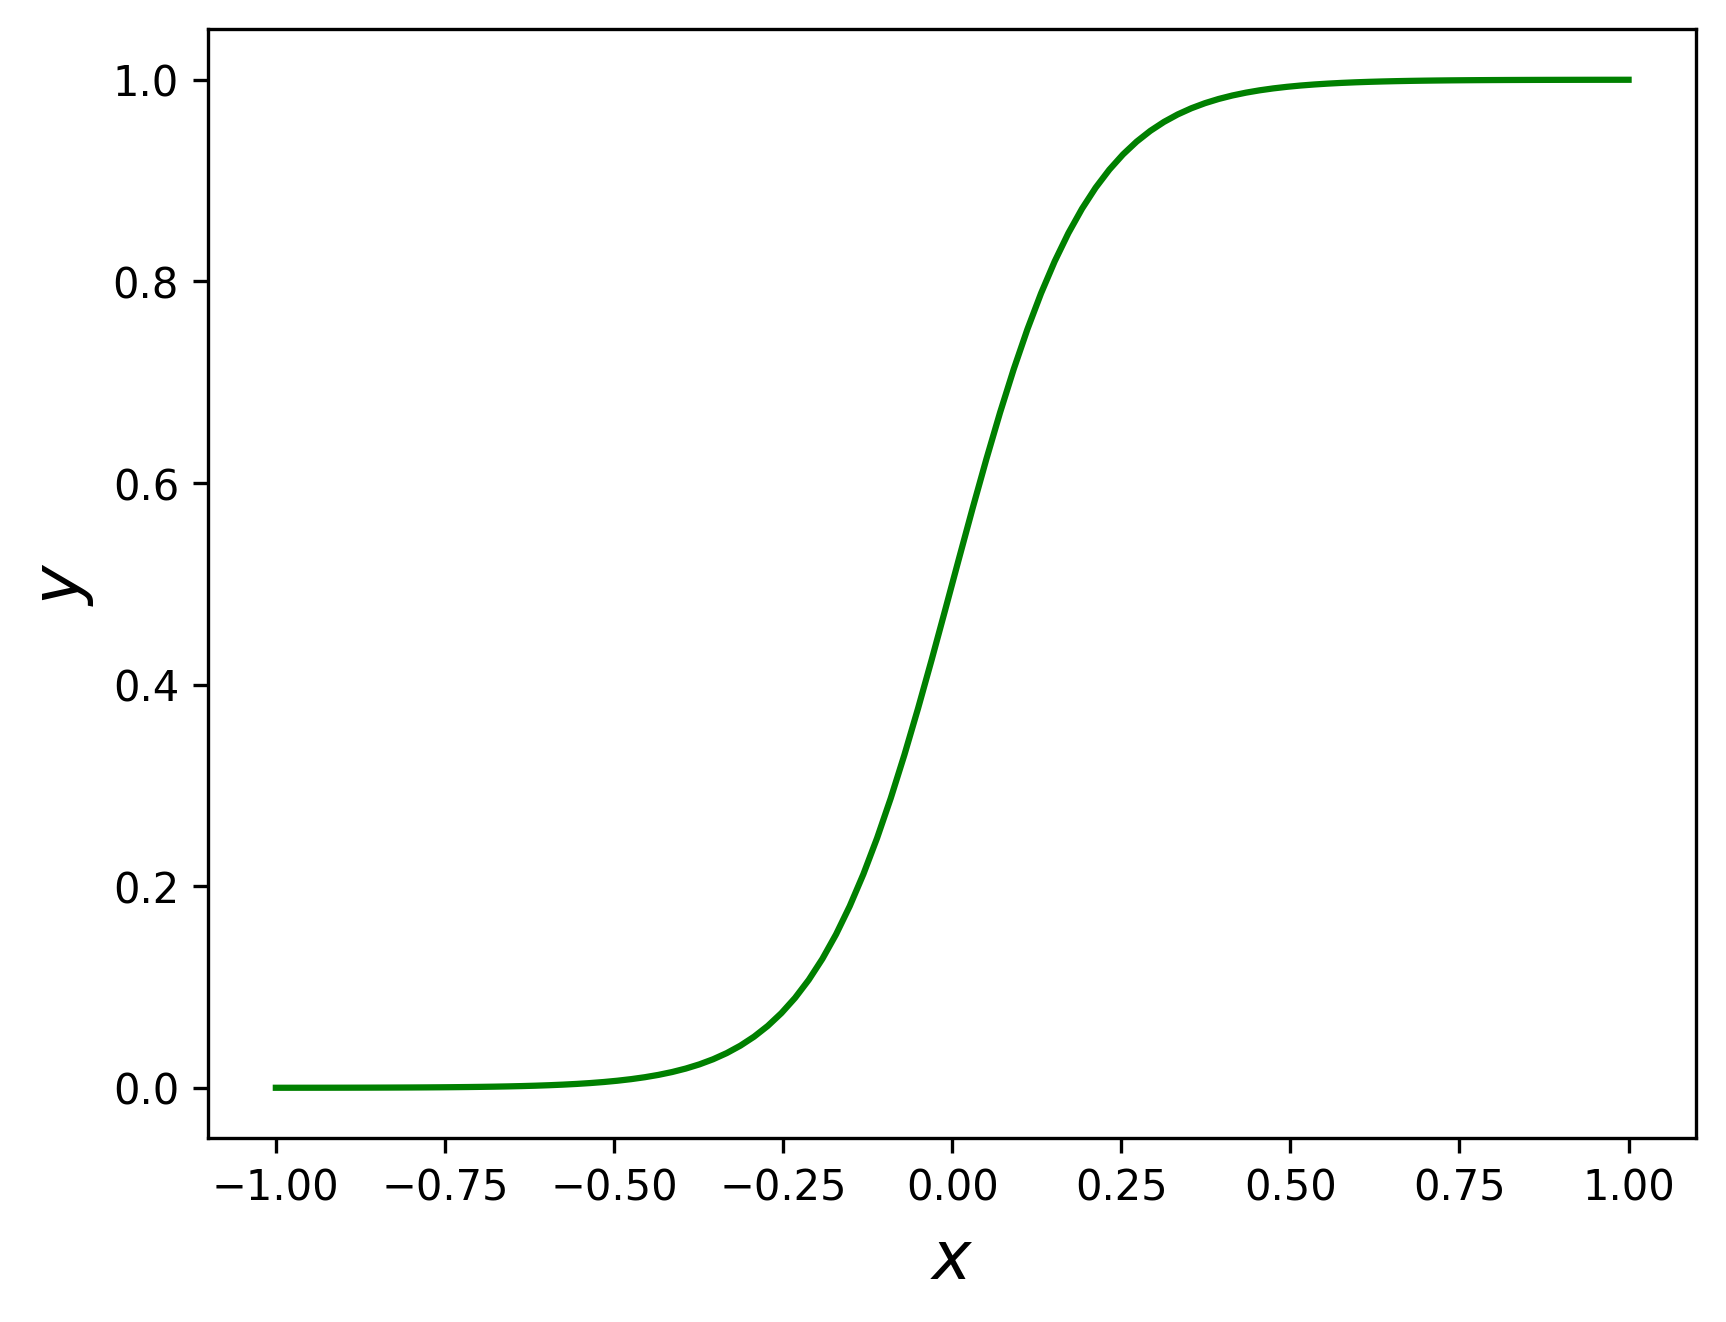
\includegraphics[width=\linewidth]{figures/sigmoidal_graf.png}
        \caption{Função Sigmoid.}
        \label{fig-1:ex-a}
    \end{subfigure}
    \hspace{30mm}
    \begin{subfigure}{0.4\linewidth}
        \centering
        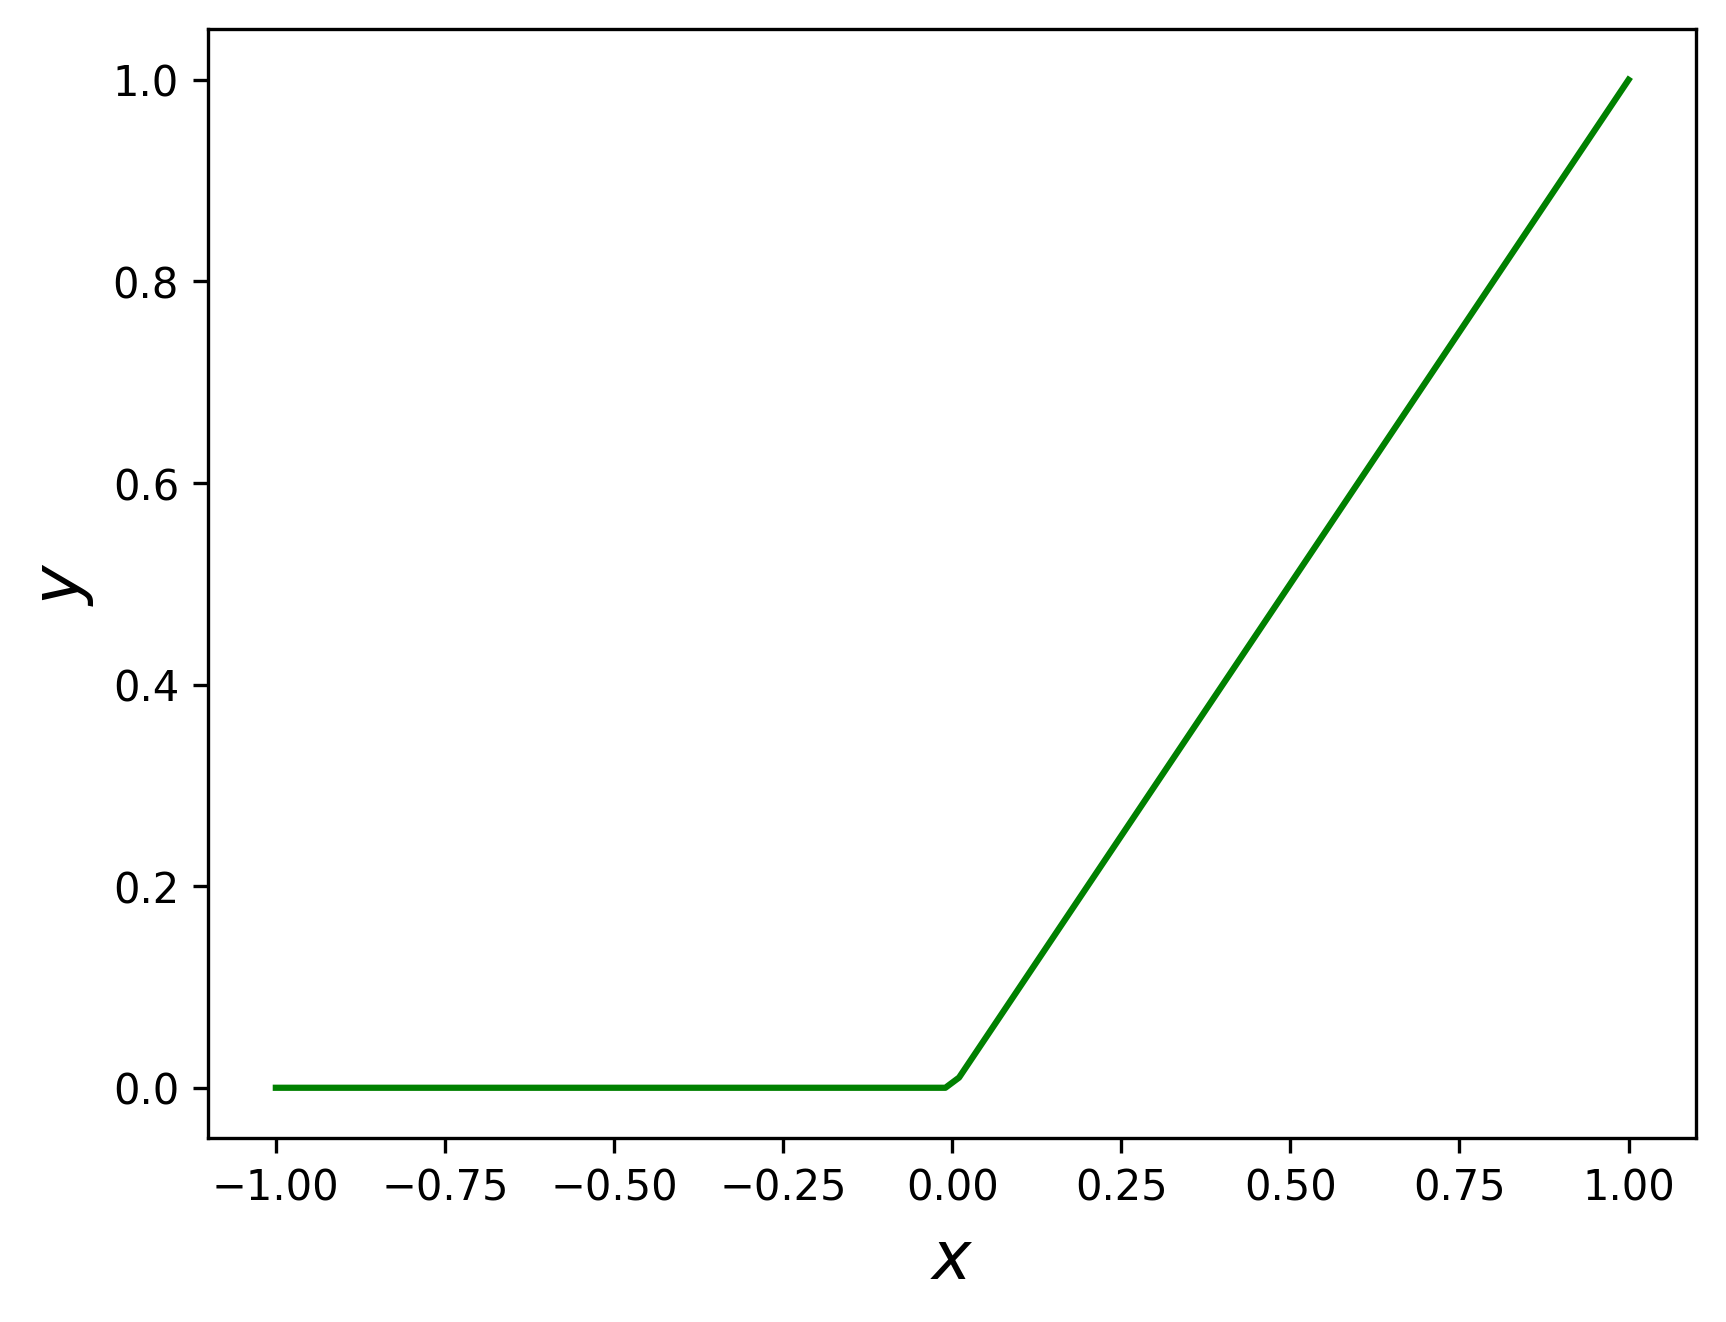
\includegraphics[width=\linewidth]{figures/relu_graf.png}
        \caption{Função ReLU.}
        \label{fig-1:ex-b}
    \end{subfigure}
    \caption*{\footnotesize Fonte: Elaboração do Autor.}
    \label{fig-1:ex-geral}
\end{figure}


A principal desvantegem na unidade de McCulloch e Pitts é a ausência de um algoritmo de aprendizagem, ou seja, uma maneira de ajustar os pesos e o viés da unidade para que este seja capaz de resolver um problema específico. Essa limitação foi superada em 1958 por Frank Rosenblatt, que propôs o \textit{Perceptron} \cite{rosemblatt}, um modelo de unidade com um algoritmo de aprendizagem capaz de ajustar os pesos e o viés da unidade. 

\subsection{Perceptron e Algoritmo de Aprendizagem}
O Perceptron é um modelo de unidade que utiliza um algoritmo de aprendizagem supervisionada para ajustar seus pesos e viés com base em um conjunto de dados ``rotulados"{\footnote{Dados rotulados são conjuntos de dados de entrada associados a saídas desejadas, ou seja, para cada conjunto de entradas, há uma saída correta conhecida.}}. O objetivo do Perceptron é encontrar uma função que mapeie corretamente as entradas para as saídas desejadas, minimizando o erro entre as previsões do modelo e os valores reais.

Para esclarecer o funcionamento do Perceptron e do algoritmo de aprendizagem, é proposto o Exemplo \ref{ex1}.

\begin{exemplo}
\label{ex1}
Um investidor busca decidir qual ação adquirir com base nas variáveis: o valor é caro?, é confiável? e é volátil?. Para isso, dispõe das avaliações de quatro colegas que também analisam essas mesmas características antes de realizar seus investimentos.
\end{exemplo}

\begin{table}[htpb]
    \centering
    \caption{Banco de dados com as avaliações dos colegas e a decisão final de compra.}
    \label{tab:1}
    $\begin{array}{ccccc}
    \hline
    & \text{valor} & \text{confiança} & \text{volatilidade} & y \\
    \hline
    x_1 & 0 & 1 & 0 & 1 \\
    \hline
    x_2 & 1 & 0 & 1 & 0 \\
    \hline
    x_3 & 1 & 1 & 1 & 0 \\
    \hline
    x_4 & 0 & 0 & 0 & 1 \\
    \hline

\end{array}$
\end{table}
Na Tabela \ref{tab:1} são apresentadas as avaliações dos colegas e a decisão final de compra em que $0$ representa ``não", $1$ representa ``sim", $x_1, \cdots, x_4$ representam as respostas de cada colegas e $y$ a decisão final de cada um. Com isso, o Perceptron terá três variáveis de entrada e como saída, a decisão sobre a compra da ação. Os pesos iniciais são definidos aleatoriamente como: $w_1 = w_2 = w_3 = 0$ e o viés como $b = 0$. A função de ativação utilizada é a função ReLU~(\ref{eq:relu}). Testando o primeiro dado de entrada $x_1 = (0,1,0)$ e $y = 1$, obtém-se: 

$$
z = x_1 \cdot w_1 + b = 0 \Rightarrow \hat{y} = \sigma(0) = 0,    
$$
o símbolo $\cdot$ representa o produto escalar entre os vetores. Como $y = 1 \neq \hat{y} = 0$, em que $\hat{y}$ é a resposta da rede definido como na equação (\ref{eq:predicao}). O Perceptron comete um erro e é necessário aplicar o algoritmo de aprendizagem (a unidade de McCulloch e Pitts pararia aqui). Para isso, define-se uma função de custo, responsável por quantificar o erro cometido durante o treinamento. Neste exemplo, utiliza-se o Erro Quadrático Médio, dado por: 
\begin{equation}
 \label{fuc:custo}
    C(w_i,b_i) = \frac{\sum_{i=1}^k(y_i - \hat{y}_i)^2}{n},   
\end{equation} 
em que $y_i$ é a resposta do dado de entrada  $x_i$ e $n$ representa a quantidade de dados presentes no conjunto de treinamento. $C(w_i,b_i)$ não depende de $w_i$ e $b_i$ explicitamente, mas sim por meio de $\hat{y}_i$, ou seja, $C(w_i,b_i) = C(\hat{y}_i(w_i,b_i))$, já que $\hat{y}_i = \sigma(z_i)$ e $z_i = x_i\cdot w_i + b_i$. No caso do Exemplo \ref{ex1}, $x_i$ e $w_i$ são vetores.

O processo de treinamento ajusta iterativamente os pesos e o viés por meio do método da Descida do Gradiente (SG - \textit{Gradient Descent}), cujo objetivo é minimizar a função de custo. Esse método utiliza as derivadas parciais da função de custo em relação aos pesos e ao viés, o que indica a direção de maior crescimento da função. Para reduzir o erro, atualizam-se os parâmetros na direção oposta ao gradiente. As derivadas são:

\begin{align}
    \frac{\partial C(w_i,b_i)}{\partial w_i} = - 2\cdot\frac{\sum_{i=1}^k(y_i - \hat{y}_i) \cdot \sigma'(z_i)\cdot x_i}{n};\\;
    \frac{\partial C(w_i,b_i)}{\partial b_i} = - 2\cdot\frac{\sum_{i=1}^k(y_i - \hat{y}_i)\cdot \sigma'(z_i)}{n}.
\end{align}
    

No o Exemplo \ref{ex1} assume-se $\sigma'(z) = 1$ para simplificação. Como a derivada aponta para a região de maior valor da função, multipica-se por $-1$ para obter a direção da região de minimização. Com isso, é obtido o Algoritmo \ref{alg:gradiente}.
\vspace{0.5cm}

\begin{algorithm}[H]
\caption{Método da Descida do Gradiente.}
\label{alg:gradiente}
\KwIn{Taxa de aprendizado $\eta$, função de custo $C(w,b)$, pesos iniciais $w_1, w_2, \dots, w_n$ e viés $b$}
\KwOut{Pesos e viés ajustados}

\BlankLine
Inicializar os pesos $w_i$ e o viés $b$ com valores pequenos aleatórios\;
\Repeat{convergência ou número máximo de iterações}{
    Calcular a saída do modelo\;
    $\hat{y}_i \leftarrow \sigma\left(\sum_{i=1}^{n} w_i \cdot x_i + b\right)$\;
    
    Calcular o erro\;
    $\Delta_w \leftarrow \frac{\sum_{i=1}^{n}(y_i - \hat{y_i})\cdot \sigma'(z_i)\cdot x_i}{n}$\;
    $\Delta_b \leftarrow \frac{\sum_{i=1}^{n}(y_i - \hat{y_i})\cdot \sigma'(z_i)}{n}$\;
    
    Atualizar os pesos e o viés\;
    $w_i \leftarrow w_i + \eta \, \Delta_w $, \quad para todo $i = 1, 2, \dots, n$\;
    $b \leftarrow b + \eta \, \Delta_b$\;
}
\Return $w_i, b$\;
\end{algorithm}
\vspace{0.5cm}
A taxa de aprendizagem ($\eta$) presente no Algoritmo \ref{alg:gradiente}  pode ser interpretada como o tamanho do passo dado em direção ao mínimo da função de custo, como mostra a Figura \ref{gradiente}. Quando o valor dessa taxa é muito pequeno, o processo de convergência torna-se mais lento, exigindo um número maior de iterações para atingir o mínimo. Por outro lado, se o passo for muito grande, o algoritmo pode ultrapassar o ponto de mínimo, dificultando ou até impedindo a convergência adequada, para o Exemplo \ref{ex1} é utilizada uma taxa de aprendizado de $0,1$.
\begin{figure}[htpb]
    \centering
    \caption{Representação da taxa de aprendizagem.}
    
\includegraphics[width=0.7\linewidth]{gradientedes.png}
    \caption*{\footnotesize Fonte: Elaboração do Autor.}
    \label{gradiente}
\end{figure}

Aplicando o Algoritmo \ref{alg:gradiente} no Exemplo \ref{ex1}, os seguintes ajustes são feitos nos pesos e no viés após uma passada pelos 4 dados presentes no banco de dados:

$$w = (-0,1, 0,1, -0,1), \ b= 0,1.$$

Verificando as previsões da rede para os parâmetros atualizados, é obtido:

\begin{itemize}
    \item[$x_1$:] $(0,1,0) \Rightarrow z = 0 \cdot (-0,1) + 1 \cdot 0,1 + 0 \cdot(-0,1) + 0,1 = 0,2 \Rightarrow \hat{y} = 1$;
    \item[$x_2$:] $(1,0,1) \Rightarrow z = -0,1 + 0+ -0,1 + 0,1 = -0,1 \Rightarrow \hat{y} = 0$;
    \item[$x_3$:] $(1,1,1) \Rightarrow z = -0,1 + 0,1 - 0,1 + 0,1 = 0 \Rightarrow \hat{y} = 0$;
    \item[$x_4$:]$ (0,0,0)\Rightarrow z = 0 + 0 + 0 + 0,1 = 0,1\Rightarrow \hat{y} = 1$.
\end{itemize}

Basta observar que $\hat{y} = \sigma(z)$ e $\sigma(z)$ é a função de ativação utilizada. Assim, após uma única época com $\eta = 0,1$ os pesos e o viés encontrados classificam corretamente todos os exemplos do conjunto de treinamento.

Comumente o banco de dados é dividido em dois conjuntos: o conjunto de treinamento e o conjunto de teste. O conjunto de treinamento é utilizado para ajustar os pesos e o viés do Perceptron, enquanto o conjunto de teste é utilizado para avaliar o desempenho do modelo em dados não vistos durante o treinamento. Essa divisão é essencial para garantir que o modelo aprenda a generalizar bem para novos dados, evitando o problema do \textit{overfitting}(na Seção \ref{overfitting}), que ocorre quando o modelo se ajusta excessivamente aos dados de treinamento, perdendo a capacidade de generalização.


\section{Redes Neurais}
\label{redesNeurais}
\begin{figure}[h!]
\centering
\caption{Organização da Seção 1.2.}
\begin{tikzpicture}[
    node distance=1.5cm,
    every node/.style={font=\small},
    main/.style={
        draw,
        rounded corners=6pt,
        thick,
        minimum width=4cm,
        minimum height=1.2cm,
        align=center
    },
    sub/.style={
        draw,
        rounded corners=4pt,
        thin,
        minimum width=3.5cm,
        minimum height=1cm,
        align=center
    },
    arrow/.style={
        -{Latex[length=3mm]},
        thick
    }
]

\node[main] (sec) {\textbf{Seção 1.2}\\Redes Neurais};

\node[sub, right =of sec] (s31) {1.2.1 Arquiteturas de Redes Neurais};
\node[sub, below left=of s31] (s32) {1.2.2 Backpropagation};
\node[sub, right=of s32] (s33) {1.2.3 Gradiente Descendente Estocástico};
\node[sub, below =of s32] (s34) {1.2.4 Overfitting};
\node[sub, right=of s34] (s35) {1.2.5 Hiperparâmetros};
\node[sub, right=of s35] (s36) {1.2.6 Regularização};
\node[sub, below=of s34] (s37) {1.2.7 Momentum};
\node[sub, right =of s37] (s38) {1.2.8 \textit{Vanishing Gradient}};
\node[sub, right=of s38] (s39) {1.2.9 \textit{Dígitos Manuscritos}};

\draw[arrow] (sec) -- (s31);
\draw[arrow] (s31) -- (s32);
\draw[arrow] (s32) -- (s33);
\draw[arrow] (s33) -- (s34);
\draw[arrow] (s34) -- (s35);
\draw[arrow] (s35) -- (s36);
\draw[arrow] (s36) -- (s37);
\draw[arrow] (s37) -- (s38);
\draw[arrow] (s38) -- (s39);

\end{tikzpicture}
\caption*{\footnotesize Fonte: Elaboração do Autor.}
\end{figure}
\label{sec_2}
Nesta seção serão apresentados os conceitos relacionados às redes neurais, sendo muito importantes para o andamento do trabalho, todos os conceitos apresentados nesta seção serão utilizados na construção da rede neural proposta na Seção \ref{sec:unet}.

As redes neurais são um ``encadeamento" de múltiplas unidades, onde a saída de uma unidade é a entrada de outra. Redes neurais podem ser organizadas em camadas: uma \textit{camada de entrada}, uma ou mais \textit{camadas ocultas} e uma \textit{camada de saída}. Cada camada é composta por várias unidades e cada unidade em uma camada está conectada a todas as unidades na camada seguinte. A Figura \ref{fig0:ex-a} ilustra a estrutura básica de uma unidade vista na Seção \ref{unidade}. Já a Figura \ref{fig0:ex-b} mostra uma rede neural com duas camadas ocultas, em que a camada de entrada tem três unidades, a primeira camada oculta tem cinco unidades, a segunda camada oculta tem quatro unidades e a camada de saída tem duas unidades. Matematicamente, é possível representar uma rede neural com duas camadas ocultas da seguinte maneira:

\begin{equation}
    \label{eq:redeNeural}
    \hat{y} = \sigma^s\left[\sum_{i=1}^4\sigma^2_i\left(\sum_{j=1}^5\sigma^1_j\left(\sum_{k=1}^3 w_{jk}^1 x_k + b_j^1\right)w_{ij}^2 + b_i^2\right)w_i^s + b^s\right],
\end{equation}
em que $\sigma^1_j$ é a função de ativação da $j$-ésima unidade da primeira camada oculta, $\sigma^2_i$ é a função de ativação da $i$-ésima unidade da segunda camada oculta e $\sigma^s$ é a função de ativação da $s$-ésima unidade da camada de saída. Os pesos e os vieses são representados por $w_{jk}^1$, $b_j^1$, $w_{ij}^2$, $b_i^2$, $w_i^s$ e $b^s$. Generalizando a notação, para uma rede neural com $L$ camadas ocultas, a saída da rede pode ser expressa como:
\begin{equation}
    \label{eq:redeNeuralGeral}
    \hat{y} = \sigma^s\left[\sum_{i_L=1}^{n_L}\sigma^L_{i_L}\left(\sum_{i_{L-1}=1}^{n_{L-1}}\sigma^{L-1}_{i_{L-1}}\left(\cdots \sum_{k=1}^{n_1}\sigma^1_k\left(\sum_{m=1}^{n_0} w_{km}^1 x_m + b_k^1\right)w_{jk}^2 + b_j^2\right)w_{ij}^L + b_i^L\right)w_i^s + b^s\right].
\end{equation}


\begin{figure}[htpb]
    \centering
    \caption{Estrutura visual básica de uma unidade e uma rede neural com duas camadas ocultas.}
    \begin{subfigure}{0.3\linewidth}
        \centering
        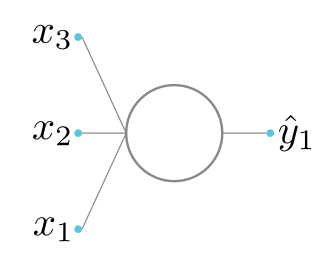
\includegraphics[width=\linewidth]{figures/perceptron.png}
        \caption{Perceptron.}
        \label{fig0:ex-a}
    \end{subfigure}
    \hspace{30mm}
    \begin{subfigure}{0.3\linewidth}
        \centering
        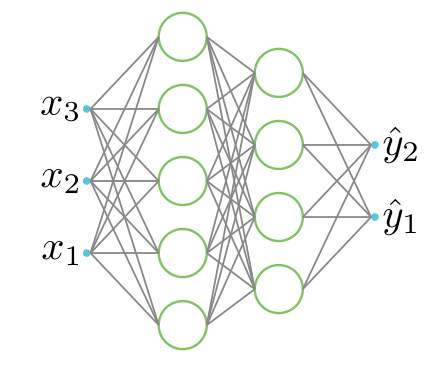
\includegraphics[width=\linewidth]{figures/rede_neural.png}
        \caption{Rede Neural com duas camadas ocultas.}
        \label{fig0:ex-b}
    \end{subfigure}
    \caption*{\footnotesize Fonte: Elaboração do Autor.}
    \label{fig:ex-geral}
\end{figure}

Outra forma de representar uma rede neural é utilizando a notação matricial, em que as entradas, os pesos e os vieses são representados por matrizes e vetores. Para uma rede neural com $n$ entradas, uma camada oculta com $m$ neurônios e uma saída, a saída da rede pode ser expressa como:

\[
\underbrace{\begin{bmatrix}
w_{11} & w_{12} & \cdots & w_{1n} \\
w_{21} & w_{22} & \cdots & w_{2n} \\
\vdots & \vdots & \ddots & \vdots \\
w_{m1} & w_{m2} & \cdots & w_{mn}
\end{bmatrix}}_{m \times n}
\underbrace{\begin{bmatrix}
x_1\\x_2\\\vdots\\x_n
\end{bmatrix}}_{n \times 1}
+
\underbrace{\begin{bmatrix}
b_1\\b_2\\\vdots\\b_m
\end{bmatrix}}_{m \times 1}
\]

Essa forma representa a saída de uma camada caso a rede tenha apenas uma camada oculta, para redes neurais com mais camadas ocultas, a notação matricial torna-se mais complexa, mas o princípio de multiplicação de matrizes e adição de vetores permanece o mesmo.

\subsection{Arquiteturas de Redes Neurais}
Existem diversas arquiteturas de redes neurais, cada uma projetada para lidar com diferentes tipos de problemas e dados. Algumas das arquiteturas mais comuns incluem (\cite{arquiteturas}): 
\begin{itemize}
    \item Redes Neurais Feedforward (FNNs): São as redes neurais mais simples, onde a informação flui em uma única direção, da camada de entrada para a camada de saída, passando pelas camadas ocultas. FNNs são amplamente utilizadas para tarefas de classificação e regressão.
    
    \item Redes Neurais Convolucionais (RNCs): São projetadas para processar dados com uma estrutura de grade, como imagens. Estas utilizam operações de convolução para extrair características espaciais dos dados de entrada. RNCs são amplamente utilizadas em tarefas de visão computacional, como reconhecimento de objetos e detecção de faces.
    
    \item Redes Neurais Recorrentes (RNNs): São projetadas para lidar com dados sequenciais, onde a saída em um determinado momento depende das entradas anteriores. RNNs possuem conexões recorrentes que permitem que informações sejam mantidas ao longo do tempo. Estas são amplamente utilizadas em tarefas como processamento de linguagem natural e reconhecimento de fala.
    
    \item Redes Neurais Generativas Adversariais (GANs): Consistem em duas redes neurais que competem entre si: um gerador e um discriminador. O gerador cria dados falsos, enquanto o discriminador tenta distinguir entre dados reais e falsos. GANs são amplamente utilizadas para geração de imagens realistas e outras tarefas criativas.
    
    \item \textit{Encoder-Decoder}: São arquiteturas que consistem em duas partes principais: o \textit{encoder}, que comprime os dados de entrada em uma representação latente, e o \textit{decoder}, que reconstrói os dados a partir dessa representação. Essas redes são amplamente utilizadas em tarefas como tradução automática e geração de texto.
\end{itemize}
É possível utilizar duas arquiteturas em conjunto, como abordado na Seção \ref{sec:unet}.

\begin{figure}[H]
    \centering
    \caption{Arquiteturas de Redes Neurais.}
    \begin{subfigure}{0.4\linewidth}
        \centering
        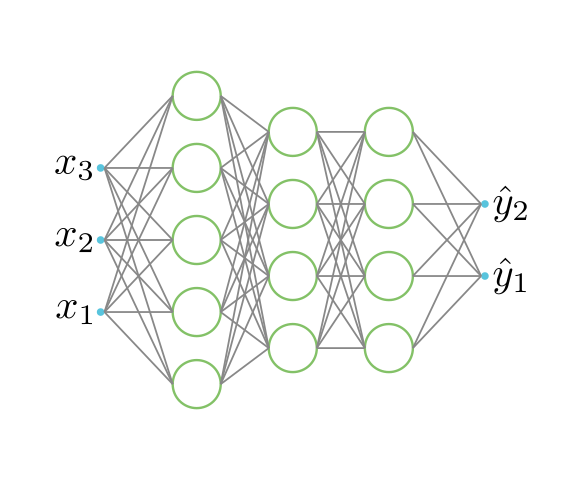
\includegraphics[width=\linewidth]{figures/FNNs.png}
        \caption{Redes Neurais \textit{Feedforward} (FNNs).}
        \label{fig:ex-a}
    \end{subfigure}
    \hspace{30mm}
    \begin{subfigure}{0.4\linewidth}
        \centering
        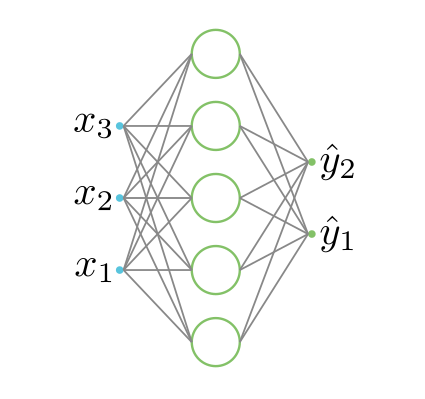
\includegraphics[width=\linewidth]{figures/RNNs.png}
        \caption{Redes Neurais Recorrentes (RNNs).}
        \label{fig:ex-b}
    \end{subfigure}
    \hspace{30mm}
    \begin{subfigure}{0.4\linewidth}
        \centering
        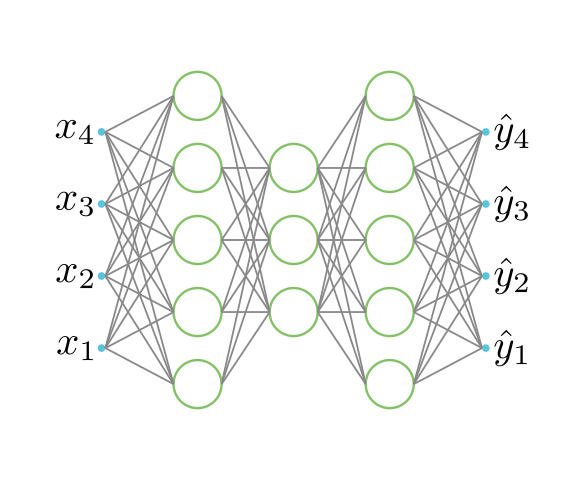
\includegraphics[width=\linewidth]{figures/EncDec.png}
        \caption{\textit{Encoder-Decoder.}}
        \label{fig:ex-c}
    \end{subfigure}

    \caption*{\footnotesize Fonte: Elaboração do Autor.}
    \label{arquiteturas}
\end{figure}

As Figuras \ref{fig:ex-a} e \ref{fig:ex-c} ilustram a arquitetura de uma Rede Neural \textit{Feedforward}, com o funcionamento semelhante ao desenvolvido na Equação (\ref{eq:redeNeuralGeral}). A Figura \ref{fig:ex-b} mostra a arquitetura de uma Rede Neural Recorrente, estas redes possuem conexões recorrentes, ou seja, a saída de uma unidade é realimentada como entrada para a mesma unidade ou para unidades anteriores, permitindo que informações sejam mantidas ao longo do tempo, por não estar no escopo deste trabalho, não serão abordados os detalhes matemáticos de funcionamento das RNNs.

\subsection{\textit{Backpropagation}}
\label{subsec:bacprop}
Assim como no perceptron, as redes neurais utilizam algoritmos de aprendizagem para ajustar seus pesos e vieses com o objetivo de minimizar uma função de custo. O algoritmo mais comum utilizado para esse propósito é o \textit{backpropagation} (retropropagação) \cite{hechtnielsen1992} e \cite{paulwerbos}, que é uma extensão do método da descida do gradiente. O \textit{backpropagation} é utilizado para calcular os gradientes da função de custo em relação aos pesos e vieses de todas as camadas da rede neural, permitindo a atualização eficiente desses parâmetros durante o treinamento. O algoritmo funciona propagando o erro da saída da rede de volta para as camadas anteriores, ajustando os pesos com base na contribuição de cada unidade para o erro total. 

Esse processo é repetido iterativamente até que a função de custo seja minimizada, resultando em uma rede neural treinada capaz de realizar previsões precisas em novos dados. Essa propagação do erro é feita utilizando a regra da cadeia do cálculo diferencial, que permite calcular as derivadas parciais de funções compostas. 
O algoritmo de \textit{backpropagation} pode ser resumido nos seguintes passos, apresentados no Algoritmo \ref{alg:backprop_etapas}.

\vspace{0.5cm}
\begin{algorithm}[H]
\caption{Etapas do treinamento via \textit{backpropagation}.}
\label{alg:backprop_etapas}
\KwIn{Dados de treinamento $(x,y)$, taxa de aprendizado $\eta$, pesos $W$ e vieses $b$}
\KwOut{Pesos $W$ e vieses $b$ atualizados}

\BlankLine
\Repeat{critério de parada (ex.: nº de épocas ou convergência)}{
    \textbf{Passo para frente:} propagar $x$ pela rede (camada a camada) e obter $\hat{y}$\;

    \textbf{Cálculo do Erro:} calcular o erro comparando $\hat{y}$ com $y$ usando uma função de custo \;

    \textbf{Passo para trás:} retropropagar o erro e calcular os gradientes $\nabla_W C$ e $\nabla_b C$ (regra da cadeia)\;

    \textbf{Atualização:} atualizar pesos e vieses (descida do gradiente)\;
    $W \leftarrow W - \eta \,\nabla_W C$\;
    $b \leftarrow b - \eta \,\nabla_b C$\;
}
\end{algorithm}

\vspace{0.5cm}
Na Figura \ref{backprop} ilustra uma rede neural simples e a equação (\ref{derivadas}) mostra o cálculo do gradiente para ajustar o peso da primeira camada ($w_1$) utilizando a regra da cadeia,

\begin{figure}[htpb]
    \centering
    \caption{Ilustração do processo de \textit{backpropagation} em uma rede neural.}
    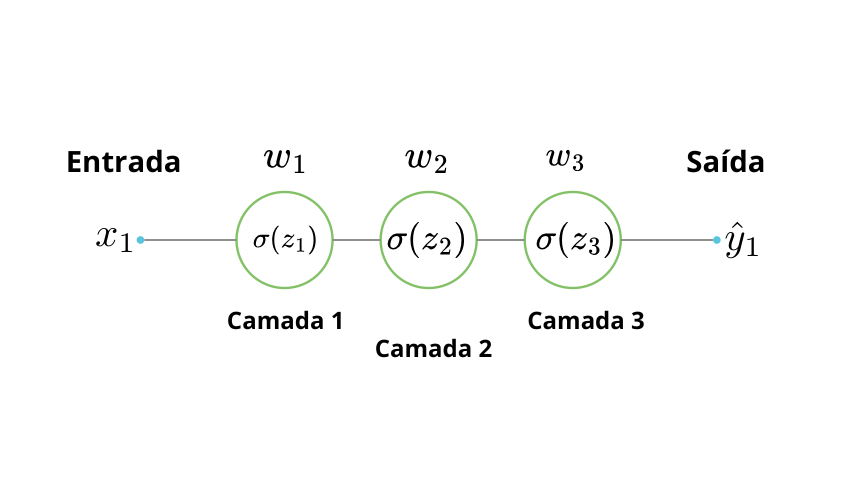
\includegraphics[width=0.7\linewidth]{figures/rede_simples.png}
    \caption*{\footnotesize Fonte: Elaboração do Autor.}
    \label{backprop}
    
\end{figure}

\begin{align}
    \label{derivadas}
    \nabla_wC = \frac{\partial C(w,b)}{\partial w_1} = \frac{C(w,b)}{\sigma(z_3)}\cdot \frac{\sigma(z_3)}{z_3} \cdot \frac{z_3}{\sigma(z_2)} \cdot \frac{\sigma(z_2)}{z_2} \cdot \frac{z_2}{\sigma(z_1)}\cdot \frac{\sigma(z_1)}{z_1} \cdot \frac{z_1}{w_1},
\end{align}
em que $z_1 = w_1\cdot x +b_1$, $z_2 = \sigma(z_1)\cdot w_2 + b_3$ e $z_3 = \sigma(z_2)\cdot w_3 + b_3$ são as saídas das camadas ocultas e $C(w,b)$ é a função de custo do erro quadrático médio, ou seja, $ C(w,b) = \frac{(\hat{y} - \sigma(z_3))^2}{n}$, $n$ sendo o número de amostras no conjunto de dados.

\subsection{Gradiente Descendente Estocástico}
\label{subsec:sgd}
O Gradiente Descendente Estocástico (SGD - Stochastic Gradient Descent) \cite{sebastianruder2016} é uma variação do método de descida do gradiente tradicional, amplamente utilizado no treinamento de redes neurais e outros modelos de aprendizado de máquina. A principal diferença entre o SGD e o método de descida do gradiente padrão é a forma como os gradientes são calculados e atualizados durante o treinamento. No método de descida do gradiente tradicional, os gradientes são calculados usando todo o conjunto de dados de treinamento, ou seja, os pesos são atualizados uma vez em cada época de treinamento, o que pode ser computacionalmente caro e demorado, especialmente para grandes conjuntos de dados. Em contraste, o SGD calcula os gradientes usando apenas uma amostra aleatória (ou um pequeno lote) do conjunto de dados em cada iteração, ou seja, caso o conjunto de dados tenha um tamanho de $1000$ e o tamanho do lote seja $10$, o SGD atualizará os pesos $100$ vezes por época. Isso torna o processo de atualização dos pesos mais rápido e eficiente, permitindo que o modelo aprenda mais rapidamente. 
Apesar da Descida do Gradiente padrão fornecer uma direção mais precisa para o mínimo global da função de custo, o SGD é capaz de chegar próximo do mínimo de forma mais rápida e eficiente.


A Figura \ref{fig:lote} ilustra como funciona o Gradiente Descendente Estocástico, em que cada seta preta indica uma atualização dos pesos do modelo. A Figura \ref{fig:sg} ilustra o caminho percorrido pelo método de descida do gradiente tradicional, enquanto a Figura \ref{fig:sgd} ilustra o caminho percorrido pelo SGD.
\begin{figure}[H]
    \centering
     \caption{Comparação entre o método de descida do gradiente tradicional e o Gradiente Descendente Estocástico.}   

    \begin{subfigure}{0.4\linewidth}
        \centering
        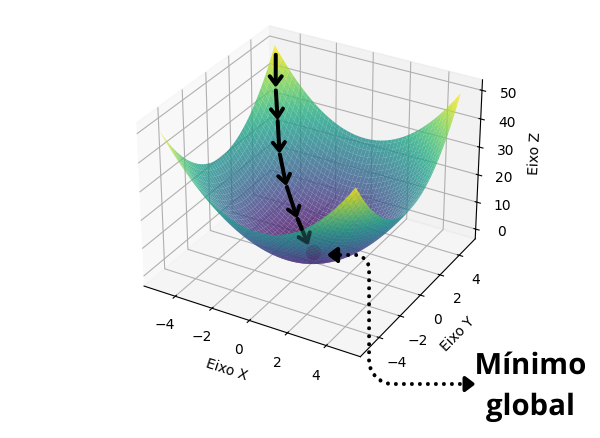
\includegraphics[width=\linewidth]{figures/SG.png}
        \caption{Descida do Gradiente Tradicional.}
        \label{fig:sg}
    \end{subfigure}
    \hspace{30mm}
    \begin{subfigure}{0.4\linewidth}
        \centering
        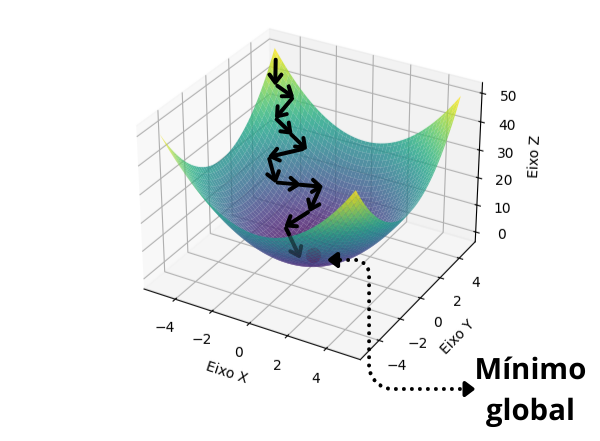
\includegraphics[width=\linewidth]{figures/SGD.png}
        \caption{Gradiente Descendente Estocástico (SGD).}
        \label{fig:sgd}
    \end{subfigure}
    \hspace{30mm }
        \begin{subfigure}{0.5\linewidth}
        \centering
        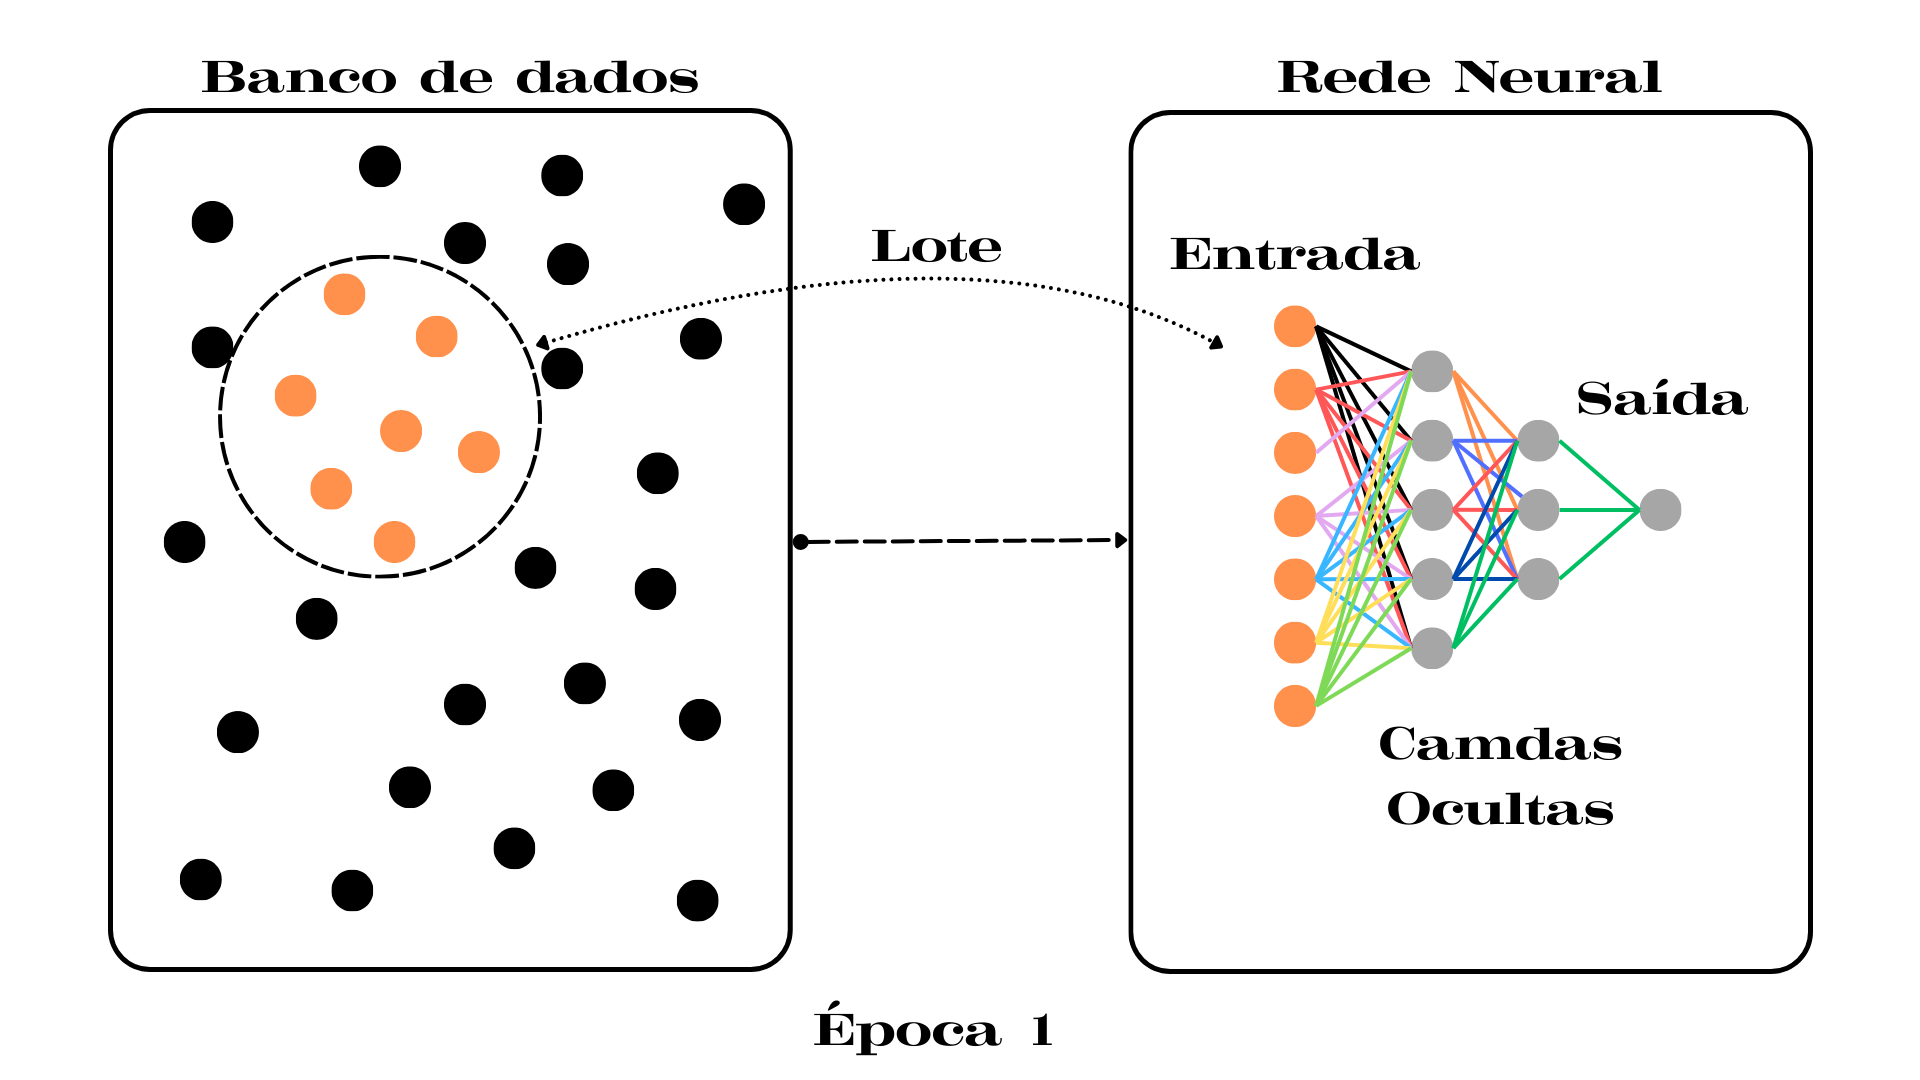
\includegraphics[width=\linewidth]{figures/lote.png}
        \caption{Separando em lotes o banco de dados para o SGD.}
        \label{fig:lote}
    \end{subfigure}
    \footnotesize
    \caption*{\footnotesize Fonte: Elaboração do Autor.}
    \label{sgd}
\end{figure}




\subsection{\textit{Overfitting}}
\label{overfitting}
O \textit{Overfitting} \cite{overfitting} (do inglês ``Sobreajuste" ou ``Ajuste Excessivo") é um problema comum em aprendizado de máquina, onde um modelo aprende os detalhes e o ruído dos dados de \mbox{treinamento} a tal ponto que este se torna incapaz de generalizar para novos dados. Isso significa que o modelo tem um desempenho excelente nos dados de treinamento, mas falha ao fazer previsões precisas em dados não vistos anteriormente. 

O \textit{overfitting} ocorre quando o modelo é muito complexo em relação à quantidade e qualidade dos dados disponíveis para treinamento. Modelos com muitos parâmetros, como redes neurais profundas, são particularmente suscetíveis ao \textit{overfitting}, especialmente quando o conjunto de dados de treinamento é pequeno ou contém ruído significativo. Na Figura \ref{fit} é apresentada uma ilustração do \textit{overfitting}, em que os pontos vermelhos são os dados de treinamento e os pontos azuis são os dados de teste, a curva verde representa um modelo que se ajusta perfeitamente aos dados de treinamento, mas falha em generalizar para novos dados, enquanto a curva azul seria um modelo ideal mais general.

\begin{figure}[htpb]
    \centering
    \caption{Ilustração do \textit{Overfitting}.}
    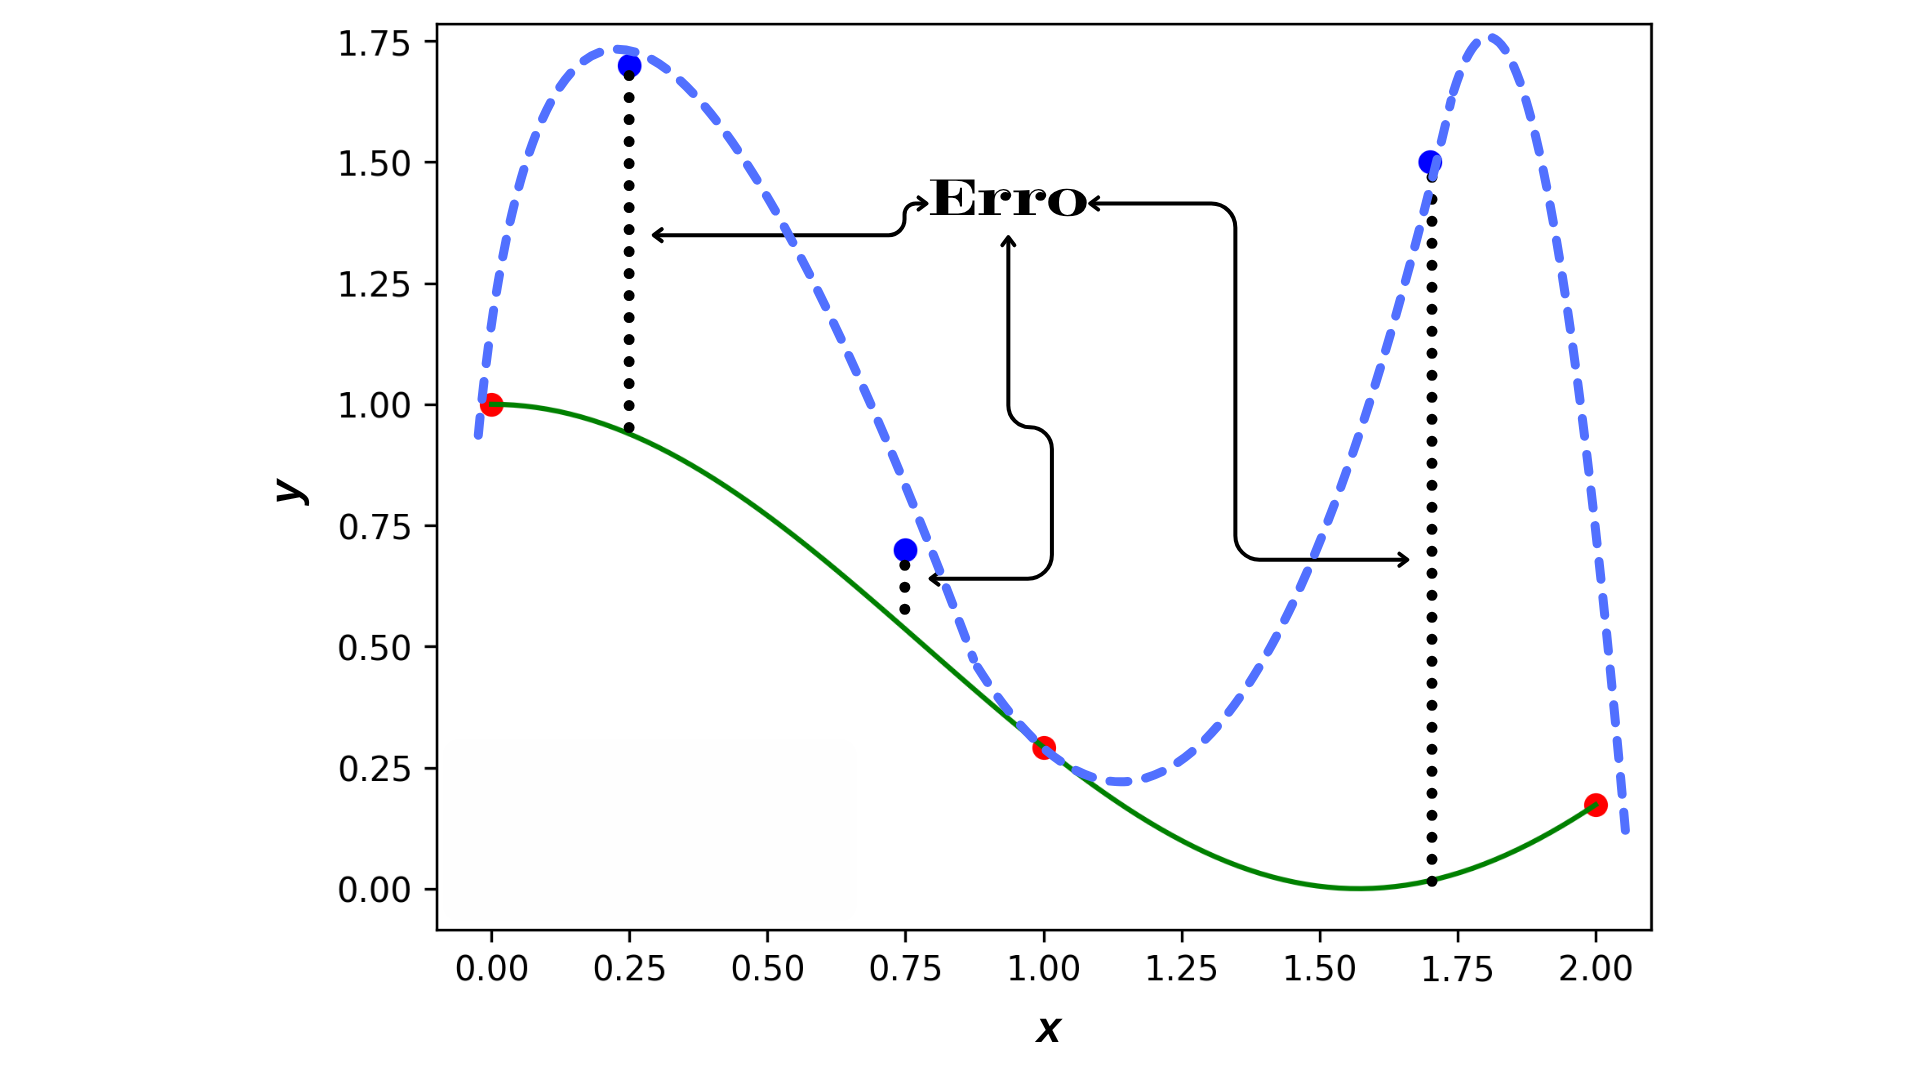
\includegraphics[width=0.7\linewidth]{figures/overffit.png}
    \caption*{\footnotesize Fonte: Elaboração do Autor.}
    \label{fit}
\end{figure}

\subsection{Hiperparâmetros}
Um algoritmo de aprendizado pode ser visto como uma função que recebe dados de treinamento como entrada e produz como saída uma função ou modelo (isto é um conjunto de funções). No entanto, na prática muitos algoritmos de aprendizado possuem parâmetros adicionais que não são aprendidos diretamente a partir dos dados de treinamento, mas que influenciam o processo de aprendizado. Esses parâmetros são chamados de hiperparâmetros e sua escolha adequada é crucial para o desempenho do modelo \cite{yoshuabengio2012}. Alguns exemplos comuns de hiperparâmetros incluem:
\begin{itemize}
    \item Taxa de Aprendizado: Controla o tamanho dos passos dados durante a atualização dos pesos do modelo. Uma taxa de aprendizado muito alta pode levar a oscilações e impedir a convergência, enquanto uma taxa muito baixa pode resultar em um processo de treinamento lento. Valores típicos para a taxa de aprendizado variam entre $0,01$ e $0,1$, dependendo do problema e do algoritmo utilizado.
    
    \item Número de Épocas: Define quantas vezes o algoritmo de aprendizado passará por todo o conjunto de dados de treinamento. Um número muito alto pode levar ao \textit{overfitting}, enquanto um número muito baixo pode resultar em \textit{underfitting} (subajuste). Uma técnica comum para determinar o número ideal de épocas é o uso do \textit{Early Stopping} (do inglês Parada Antecipada), que monitora o desempenho do modelo em um conjunto de validação e interrompe o treinamento quando o desempenho começa a piorar.
    
    \item Tamanho do Lote: Refere-se ao número de amostras de dados usadas para calcular o gradiente em cada iteração do treinamento. Tamanhos de lote menores podem levar a atualizações mais ruidosas, enquanto tamanhos maiores podem resultar em um treinamento mais estável, embora mais lento. Os valores escolhidos geralmente variam entre $1$ e $32$, sendo que valores acima de $10$ tiram proveito da Unidade Central de Processamento (do inglês \textit{Central Processing Unit} - CPU) e da Unidade de Processamento Gráfico (do inglês \textit{Graphics Processing Unit} - GPU), que oferece ganho de velocidade dos produtos matriz-matriz em relação aos produtos matriz-vetor.
    
    \item Arquitetura do Modelo: Inclui o número de camadas, o número de unidades em cada camada e o tipo de funções de ativação utilizadas. Modelos mais complexos podem capturar padrões mais sofisticados, mas também são mais propensos ao \textit{overfitting}.
\end{itemize}

\subsection{Regularização}
\label{regularizacao}
A regularização \cite{regularizacao} é uma técnica utilizada para prevenir o \textit{overfitting} em modelos de aprendizado de máquina, adicionando uma penalidade à função de custo que o modelo tenta minimizar durante o treinamento. Essa penalidade incentiva o modelo a manter os pesos dos parâmetros pequenos, o que ajuda a evitar que ele se ajuste excessivamente aos dados de treinamento. Existem várias técnicas de regularização, sendo as mais comuns:
\begin{itemize}
    \item Regularização L1 (Norma 1): Adiciona uma penalidade proporcional à soma dos valores absolutos dos pesos dos parâmetros à função de custo. Isso pode levar a soluções esparsas, onde alguns pesos são reduzidos a zero, efetivamente removendo certas características do modelo. A equação da função de custo com regularização L1 é dada por:
    \begin{equation}
        \label{eq:l1}
        C(w,b) = C_0(w,b) + \frac{\lambda}{n} \sum_{i} |w_i|,
    \end{equation}
    em que $C_0(w,b)$ é a função de custo original, $\lambda$ é o parâmetro de regularização que controla a força da penalidade, $w_i$ são os pesos dos parâmetros do modelo e $n$ é o número de amostras no conjunto de dados.
    
    \item Regularização L2 (Norma 2): Adiciona uma penalidade proporcional à soma dos quadrados dos pesos dos parâmetros à função de custo. Isso incentiva o modelo a distribuir os pesos de forma mais uniforme, evitando que alguns pesos se tornem muito grandes. A equação da função de custo com regularização L2 é dada por:
    \begin{equation}
        \label{eq:l2}
        C(w,b) = C_0(w,b) + \frac{\lambda}{n} \sum_{i} w_i^2,
    \end{equation}
    em que os termos são definidos da mesma forma que na regularização L1.
    
    \item \textit{Dropout}: Durante o treinamento, essa técnica desativa aleatoriamente uma fração das unidades em cada camada da rede neural para cada época. Isso força a rede a aprender representações mais robustas e reduz a dependência de unidades específicas, ajudando a prevenir o \textit{overfitting}. Em termos gerais, ao aplicar o \textit{dropout} estamos treinando uma coleção de sub-redes dentro da rede original, o que pode promover a generalização do modelo.
    \begin{figure}[htpb]
        \centering
        \caption{Ilustração do \textit{Dropout} removendo 60\% das unidades aleatoriamente durante uma época de treinamento.}
        
\includegraphics[width=0.7\linewidth]{img_dropout.png}
        \caption*{\footnotesize Fonte: Elaboração do Autor.}
        \label{dropout}
    \end{figure}
    
    \item \textit{Early Stopping} (Parada Antecipada): Monitora o desempenho do modelo em um conjunto de validação durante o treinamento e interrompe o processo quando o desempenho começa a piorar. Isso evita que o modelo continue a se ajustar aos dados de treinamento além do ponto ideal. Como ilustrado na Figura \ref{earlystopping}, o ponto de parada ideal é onde a acurácia na validação começa a diminuir, indicando o início do \textit{overfitting}.
    \begin{figure}[htpb]
        \centering
        \caption{Ilustração do \textit{Early Stopping}.}
        
\includegraphics[width=0.7\linewidth]{earlystopping.png}
        \caption*{\footnotesize Fonte: Adaptado de \cite{regularizacao}.}
        \label{earlystopping}
    \end{figure}
\end{itemize}

\subsection{\textit{Momentum}}
O \textit{Momentum} (Momento) \cite{momentum} é uma técnica utilizada para acelerar o processo de treinamento de redes neurais, especialmente em situações onde a função de custo apresenta regiões íngremes ou planas. A ideia principal do \textit{momentum} é acumular uma média ponderada dos gradientes anteriores para suavizar as atualizações dos pesos, permitindo que o modelo mantenha uma direção consistente durante o treinamento. Isso ajuda a evitar oscilações e acelera a convergência para o mínimo da função de custo. Dada uma função de custo $C(w, b)$ a ser minimizada, o \textit{momentum} clássico é definido por:

\begin{equation}
    \begin{cases}
        v_{t+1} = \beta v_t-1 +  \epsilon \nabla C(w_t, b_t) \\
        \theta_{t+1} = \theta_t + v_{t+1},
    \end{cases}
\end{equation}
em que $\epsilon > 0$ é a taxa de aprendizagem, $\beta \in [0,1]$ é o coeficiente de \textit{momentum}, $v_t$ é a velocidade acumulada no tempo $t$, $\theta_t = (w_t, b_t)$ representa os parâmetros do modelo (pesos e vieses) no tempo $t$ e $\nabla C(w_t, b_t)$ é o gradiente da função de custo em relação aos parâmetros do modelo. O coeficiente de \textit{momentum} $\beta$ controla a influência dos gradientes anteriores nas atualizações atuais. Valores típicos para $\beta$ variam entre $0,9$ e $0,99$, com valores mais altos dando mais peso aos gradientes passados.

\textcolor{red}{Colocar um subseção do ADAM, que é uma variação do Momentum.}

\subsection{\textit{Vanishing Gradient}}
\label{vanishing}
O problema do \textit{vanishing gradient} (gradiente que desaparece)  ocorre durante o treinamento de redes neurais profundas, em que os gradientes calculados durante o processo de \textit{backpropagation} tornam-se extremamente pequenos à medida que são propagados para as camadas mais próximas da entrada. Isso acontece devido à multiplicação repetida de pequenas derivadas associadas às funções de ativação e aos pesos das camadas. Como resultado, os pesos das camadas iniciais da rede recebem atualizações insignificantes, dificultando o aprendizado efetivo dessas camadas. Como neste trabalho serão utilizadas redes neurais profundas, é importante entender o impacto do problema do \textit{vanishing gradient} e as técnicas para mitigá-lo.
\begin{exemplo}
\label{ex2}
Considere uma rede neural profunda com várias camadas ocultas, em que cada camada utiliza a função de ativação sigmoid logística, definida como:
\begin{equation}
    \sigma(z) = \frac{1}{1 + e^{-z}}.
\end{equation}
A derivada dessa função é dada por:
\begin{equation}
    \sigma'(z) = \sigma(z)(1 - \sigma(z)).
\end{equation}


Durante o processo de backpropagation, o gradiente da função de custo em relação aos pesos das camadas iniciais é calculado utilizando a regra da cadeia. Isso envolve a multiplicação das derivadas das funções de ativação de cada camada, como mostra a equação (\ref{derivadas}). Como a derivada da função sigmoid é sempre menor que 0,25 (o valor máximo ocorre em $z=0$), a multiplicação repetida dessas pequenas derivadas resulta em gradientes que se tornam cada vez menores à medida que são propagados para trás através das camadas da rede. Por exemplo, se uma rede possui 10 camadas ocultas, o gradiente pode ser reduzido a um valor extremamente pequeno, como $10^{-6}$ ou menor, tornando as atualizações dos pesos nas camadas iniciais praticamente insignificantes.
\end{exemplo}
\begin{figure}[htpb]
    \centering
    \caption{Gráfico da derivada da função sigmoid logística.}
    
\includegraphics[width=0.5\linewidth]{sigmoid_prime.png}
    \caption*{\footnotesize Fonte: Elaboração do Autor.}
    \label{sigmoide}
\end{figure}


O problema do \textit{vanishing gradient} é particularmente comum em redes neurais recorrentes (RNNs) e em redes \textit{feedforward} profundas que utilizam funções de ativação como a sigmoid ou a tangente hiperbólica. Para contornar o problema do \textit{vanishing gradient}, várias técnicas podem ser empregadas, incluindo:
\begin{itemize}
    \item Funções de Ativação Alternativas: Funções de ativação como ReLU e suas variantes (Leaky ReLU, Parametric ReLU) têm derivadas constantes para valores positivos, o que ajuda a manter os gradientes maiores durante o \textit{backpropagation}.
    \item \textit{Batch Normalization}: Normaliza as ativações de cada camada durante o treinamento, o que pode ajudar a estabilizar os gradientes e acelerar o processo de aprendizado.
\end{itemize}

\subsection{Dígitos Manuscritos}
Para exemplicar o funcionamento de como uma rede neural faz o reconhecimento de imagens, considere a tarefa de classificação de dígitos manuscritos utilizando o conjunto de dados MNIST \cite{mnist}. O conjunto de dados MNIST consiste em $70.000$ imagens em escala de cinza de dígitos manuscritos (0 a 9), cada uma com uma resolução de $28\times28$ pixels, como mostra a Figura \ref{mnist}.  

\begin{figure}[htpb]
    \centering
    \caption{Exemplos de dígitos manuscritos do conjunto de dados MNIST.}
    
\includegraphics[width=0.7\linewidth]{mnist.png}
    \caption*{\footnotesize Fonte: Adaptado de \cite{mnist}.}
    \label{mnist}
\end{figure}

Cada imagem é representada como uma matriz de $28\times28$, em que cada pixel tem um valor de intensidade entre 0 (preto) e 255 (branco). Para o reconhecimento dos digitos utilizou-se uma rede \textit{feedforward} e os métodos presententes em (\ref{subsec:bacprop}), (\ref{subsec:sgd}), (\ref{regularizacao}) e (\ref{vanishing}) para o treinamento e otimização dos pesos.  Para compor a camada de entrada da rede neural, cada imagem é ``achatada" em um vetor de 784 elementos $(28\times28 = 784)$, onde cada elemento corresponde à intensidade de um pixel. O objetivo da rede neural \textit{feedforward} com camadas totalmente conectadas é aprender a classificar corretamente cada imagem em uma das 10 classes correspondentes aos dígitos de 0 a 9. Como a camada de saída da rede neural deve ter 10 unidades (um para cada classe), a arquitetura da rede pode ser definida como [784, 30, 9], onde a camada de entrada tem 784 unidades, a camada oculta tem 30 unidades (valor escolhido aleatóriamente) e a camada de saída tem 9 unidades, como mostra a Figura \ref{mnist_rede}. 

\begin{figure}[htpb]
    \centering
    \caption{Arquitetura da rede neural para classificação de dígitos manuscritos. Inicialmente, é enviado o número de pixels da imagem (784) para a camada de entrada (unidade $x_{784} = 0,4$ intensidade do pixel), que é processada por uma camada oculta com 30 unidades, e a camada de saída tem 9 unidades, correspondendo às 10 classes de dígitos (0 a 9).}
    
\includegraphics[width=0.7\linewidth]{MNIST.png}
    \caption*{\footnotesize Fonte: Elaboração do Autor.}
    \label{mnist_rede}
\end{figure}



A função de ativação utilizada é a função sigmoid logística vista na equação (\ref{eq:sigmoid}), que é comumente usada em tarefas de classificação. A saída da rede é um vetor de $10$ elementos, em que cada elemento representa a probabilidade da imagem pertencer a uma das classes de dígitos. A classe com a maior probabilidade é escolhida como a previsão da rede para a imagem de entrada (para a Figura \ref{mnist_rede} a resposta da rede é $5$, que foi a unidade com a maior probabilidade). ]

% Outra forma de interpretar a saída da rede é utilizando a Função Limiar (Equação \ref{funcaoLimiar}) e quatro neurônios na camada de saída, em que cada neurônio representaria um valor binário ($0$ ou $1$), então caso a rede recebesse o dígito $9$ e sua respota fosse correta, a saída seria $1001$ que é nove em binário. O problema de treinar uma rede neural com essa arquitetura é que ela estaria mais sucetível a erro, pois errando qualquer uma das quatro saídas, a resposta seria incorreta, enquanto utilizando a função sigmoid logística, mesmo que a rede errasse a previsão da classe correta, ela poderia ainda assim atribuir uma probabilidade alta para a classe correta, o que é mais tolerante a erros.

Para o treinamento da rede é utilizado o algoritmo de \textit{backpropagation} (Algoritmo \ref{alg:backprop_etapas}) e o Gradiente Descendente Estocástico, com uma taxa de aprendizagem de $0,1$ e a normalização $L1$ visto na equação (\ref{eq:l1}). O treinamento é realizado para 30 épocas. O banco de dados é dividido em um conjunto de treinamento com $60.000$ imagens e um conjunto de teste com $10.000$ imagens, aleatóriamente. Após o treinamento, a rede neural é avaliada no conjunto de teste para medir sua acurácia, que é a proporção de previsões corretas em relação ao total de previsões feitas:
\begin{equation}
    \label{eq:acuracia}
    \text{Acurácia} = \frac{\text{Número de Previsões Corretas}}{\text{Número Total de Previsões}}.
\end{equation}
A Figura \ref{fluxo} mostra o fluxo de dados durante o processo de treinamento e avaliação da rede neural para classificação de dígitos manuscritos.

\begin{figure}[htpb]
    \centering
    \caption{Fluxo de dados durante o processo de treinamento e avaliação da rede neural.}
    
\includegraphics[width=0.9\linewidth]{fluxo.png}
    \caption*{\footnotesize Fonte: Elaboração do Autor.}
    \label{fluxo}
\end{figure}

Com as configurações mencionadas, a rede neural alcançou uma acurácia de aproximadamente 95\% no conjunto de teste, o que indica que esta foi capaz de aprender a classificar corretamente a maioria das imagens de dígitos manuscritos.
\newpage
\section{Rede Neural para Análise de Imagens}
\begin{figure}[h!]
\centering
\caption{Organização da Seção 1.3.}
\begin{tikzpicture}[
    node distance=1.5cm,
    every node/.style={font=\small},
    main/.style={
        draw,
        rounded corners=6pt,
        thick,
        minimum width=4cm,
        minimum height=1.2cm,
        align=center
    },
    sub/.style={
        draw,
        rounded corners=4pt,
        thin,
        minimum width=3.5cm,
        minimum height=1cm,
        align=center
    },
    arrow/.style={
        -{Latex[length=3mm]},
        thick
    }
]

\node[main] (sec) {\textbf{Seção 1.3}\\Rede Neural para Análise de Imagens};

\node[sub, right =of sec] (s31) {1.3.1 Córtex Visual Humano e \\Visão Computacional};
\node[sub, below left=of s31] (s32) {1.3.2 Redes Neurais Convolucionais};
\node[sub, right=of s32] (s33) {1.3.3 Convolução};
\node[sub, below =of s32] (s34) {1.3.4 \textit{Kernel} Multicamadas};
\node[sub, right=of s34] (s35) {1.3.5 \textit{Padding}};
\node[sub, right=of s35] (s36) {1.3.6 \textit{Stride}};
\node[sub, below=of s34] (s37) {1.3.7 \textit{Pooling}};
\node[sub, right =of s37] (s38) {1.3.8 Convolução Transposta};

\draw[arrow] (sec) -- (s31);
\draw[arrow] (s31) -- (s32);
\draw[arrow] (s32) -- (s33);
\draw[arrow] (s33) -- (s34);
\draw[arrow] (s34) -- (s35);
\draw[arrow] (s35) -- (s36);
\draw[arrow] (s36) -- (s37);
\draw[arrow] (s37) -- (s38);
\end{tikzpicture}
\caption*{\footnotesize Fonte: Elaboração do Autor.}
\end{figure}
\subsection{Córtex Visual Humano e Visão Computacional}
\label{CoViHu}
O córtex visual humano é a parte do cérebro responsável pelo processamento das informações visuais recebidas pelos olhos \cite{FisioHumana}. Este está localizado na parte posterior do cérebro, na região occipital. O córtex visual é organizado em várias áreas, cada uma especializada em processar diferentes aspectos da visão, como cor, forma, movimento e profundidade. Essas áreas trabalham em conjunto para interpretar e compreender o mundo visual ao nosso redor. A estrutura do córtex visual é altamente complexa, com bilhões de unidades interconectados que formam redes neurais intrincadas. Essas redes são capazes de aprender e adaptar-se com base nas experiências visuais, permitindo-nos reconhecer objetos, rostos e padrões visuais de maneira eficiente. Uma característica importante do córtex visual é a presença de campos receptivos, que são regiões específicas do campo visual onde a estimulação de uma unidade resulta em uma resposta. Esses campos receptivos são organizados de forma hierárquica, com unidades em níveis mais baixos respondendo a características simples, como bordas e texturas, enquanto unidades em níveis mais altos respondem a características mais complexas, como formas e objetos completos.
É por meio desse mecanismo e também pela capacidade de aprendizagem que o ser humano é capaz de reconhecer e interpretar o mundo visual ao seu redor.

Traduzir a visão para uma representação digital é um processo extremamente complexo. Em parte, porque é um problema inverso, no qual busca-se recuperar algumas variáveis desconhecidas a partir de informações insuficientes para especificar completamente a solução. Portanto, deve-se recorrer a modelos baseados na física, modelos probabilísticos ou aprendizado de máquina com grandes conjuntos de exemplos para resolver ambiguidades entre possíveis soluções. Entretanto, modelar o mundo visual em toda a sua rica complexidade é muito mais difícil do que, por exemplo, modelar o trato vocal que produz sons da fala \cite{szeliski2010}. 

É surpreendente que humanos e animais façam isso com tanta facilidade, enquanto algoritmos de visão computacional são tão propensos a erros. Pessoas que nunca trabalharam na área frequentemente subestimam a dificuldade do problema. Essa percepção equivocada de que a visão deveria ser fácil remonta aos primeiros dias da inteligência artificial, quando se acreditava inicialmente que as partes cognitivas (prova lógica e planejamento) da inteligência eram intrinsecamente mais difíceis do que os componentes perceptivos \cite{Muller2008ReviewBoden}\footnote{\cite{Muller2008ReviewBoden} cita \cite{Crevier1993AI} como a fonte original. Entretanto o artigo original foi escrito por Seymour Papert (1966) e envolveu uma turma de estudantes.}. 


Uma imagem virtual é uma representação visual de um objeto, cena ou conceito, composta por uma matriz de pixels que contém informações sobre cor e intensidade. Cada pixel é uma célula na matriz da imagem que possui um valor específico. As imagens podem ser em escala de cinza, em que cada pixel tem um valor de intensidade entre 0 (preto) e 255 (branco), como mostra a Figura \ref{img_cinza}, ou em cores, em que cada pixel é representado por uma combinação de valores para as cores primárias (vermelho, verde e azul - RGB), uma imagem colorida pode ser interpretada como a sobreposição de três matrizes, cada matriz representando uma das cores primárias. 

\begin{figure}[htpb]
    \centering
    \caption{Exemplo de uma imagem/matriz $10\times10$ em escala de cinza, em que cada pixel tem um valor de intensidade entre 0 (preto) e 255 (branco).}
    
\includegraphics[width=0.6\linewidth]{matriz_escala_cinza.png}
    \caption*{\footnotesize Fonte: Elaboração do Autor.}
    \label{img_cinza}
\end{figure}


\subsection{Redes Neurais Convolucionais}
\label{redesConvolucionais}
As redes neurais convolucionais (RNCs ou do ingles \textit{Convolutional Neural Networks} - CNNs) são uma classe especial de redes neurais projetadas para processar dados com uma estrutura de grade e que tenham uma relação de vizinhaça entre os elementos, como imagens~\cite{medium}, foram baseadas do Cortex Visual Humano~(\ref{CoViHu}). Estas são amplamente utilizadas em tarefas de visão computacional, como reconhecimento de objetos, detecção de faces e segmentação\footnote{Posteriormente será exeplicado por que o termo segmentação pode ser trocado por máscara.} de imagens. As RNCs são inspiradas na organização do córtex visual, onde diferentes regiões do cérebro são responsáveis por processar diferentes partes do campo visual.

\subsection{Convolução}
\begin{exemplo}
\label{ex:convolucao}
Supondo que na tentativa de localizar uma nave com um sensor a laser \cite{Goodfellow-et-al-2016}, este sensor retorna uma única saída $x(t)$, a posição da nave no tempo $t$. $x(t)$ e $t$ são valores reais, ou seja, é possível adquirir diferentes leituras do sensor em qualquer instante de tempo. Supondo que o sensor seja ruidoso, para obter pouco ruído da estimativa da posição da nave é possível fazer várias medições e calcular a média destas, entretanto, medições mais recentes são mais relevantes, então, pode-se fazer uma média ponderada que dê pesos às medições mais recentes. Seja esta média a função $w(a)$,em que $a$ é o tempo em que a medição foi obtida. Ao aplicar $w(a)$ à $x(t)$, para todo $t$, é obtida a função $s$, que é a estimativa suavizada da posição da nave, ou seja:
\begin{equation}
    s(t) = \int x(a)w(t-a)da.
\end{equation}
\end{exemplo}
Essa operação é chamada de convolução \cite{convolucao}. A operação de convolução é tipicamente denotada com um asterístico:
$$
s(t) = (x*w)(t).
$$

No exemplo \ref{ex:convolucao}, é preciso que $w$ seja uma função densidade de probabilidade válida para que a saída seja uma méida ponderada e $w$ precisa ser igual a zero para $a < 0$. Estas restrições são particulares do exemplo, em geral, convolução é definida para quaisquer funções e integrais. 

Na terminologia da rede convolucional, o primeiro termo ($x$) é frequentemente chamado de \textit{input} (entrada), o segundo termo ($w$) é chamado de \textit{kernel} (núcleo) ou filtro, e o resultado ($s$) é chamado de \textit{feature map} (mapa de características).



% Sejam $x(t)$ e $w(t)$ funções reais contínuas por partes e integráveis, respectivamente denominadas de \textit{sinal} e \textit{kernel}, em que $t$ pode ser representado pela variável tempo, a convolução entre essas duas funções é definida como:
A operação de convolução é comumente aplicada a dados provenientes de domínios discretos (dados de computador). Se ($x$) e ($w$) são definidas somente para valores inteiros de $t$, a convolução discreta é definida por:
\begin{equation}
    s(t) = (x*w)(t) = \sum_{a=-\infty}^{\infty} x(a)w(t-a),
\end{equation}
em muitos materiais, a convolução discreta pode ser representada por:
$$
s[t] = (x*w)[t] = \sum_{a=-\infty}^{\infty} x[a]w[t-a]
$$
\begin{exemplo}
    Seja $f(t) = e^{-t}u(t)$ e $g(t) = u(t)$, onde $u(t)$ é a função limiar equação (\ref{funcaoLimiar}). A convolução $(f*g)(t)$ é dada por:
    $$
    (f*g)(t) = \int_{-\infty}^{\infty} e^{-a}u(a)u(t-a)da.
    $$
Para $t < 0$, a função limiar $u(t-a)$ é zero para todos os valores de $a$, o que resulta em $(f*g)(t) = 0$. Para $t \geq 0$, a função limiar $u(t-a)$ é igual a 1 para $a \leq t$ e zero para $a > t$. Portanto, a convolução pode ser reescrita como:
$$
(f*g)(t) = \int_{0}^{t} e^{-a} da.
$$
Calculando a integral, obtem-se:
$$
(f*g)(t) = \left[-e^{-a}\right]_{0}^{t} = 1 - e^{-t}.
$$
Portanto, a convolução entre as funções $f(t)$ e $g(t)$ é dada por:
\begin{equation}
    (f*g)(t) = \begin{cases}
    0, & t < 0 \\
    1 - e^{-t}, & t \geq 0
    \end{cases}
\end{equation}

\end{exemplo}
Intuitivamente, a função $g$ é invertida e deslocada por $t$ e depois multiplicada ponto a ponto com a função $f$, e o resultado é integrado sobre todo o domínio contínuo. Para domínios discretos, o Exemplo \ref{ex:conv_discreta} mostra o processo de convolução entre duas sequências finitas. 

\begin{exemplo}
    \label{ex:conv_discreta}
    Seja $x[n] = \{1, 2, 3\}$ e $w[n] = \{0, 1\}$, em que $x[0] = 1$, $x[1] = 2$, $x[2] = 3$, $w[0] = 0$ e $w[1] = 1$ e $w[n] = x[n] = 0$ para outros valores de $n$. A convolução $(x*w)[n]$ é dada por:
    \begin{align*}
        s[n] = (x*w)[n] = \sum_{a=0}^{3} x[a]w[n-a].
    \end{align*}
Calculando os valores para cada $n$, obtém-se:
    \begin{align*}
        (n = 0) \quad (x*w)[0] &= x[0]w[0] + x[1]w[-1] + x[2]w[-2] = 1 \cdot 0 + 2 \cdot 0 + 3 \cdot 0 = 0 \\
        (n = 1) \quad (x*w)[1] &= x[0]w[1] + x[1]w[0] + x[2]w[-1] = 1 \cdot 1 + 2 \cdot 0 + 3 \cdot 0 = 1 \\
        (n = 2) \quad (x*w)[2] &= x[0]w[2] + x[1]w[1] + x[2]w[0] = 1 \cdot 0 + 2 \cdot 1 + 3 \cdot 0 = 2 \\
        (n = 3) \quad (x*w)[3] &= x[0]w[3] + x[1]w[2] + x[2]w[1] = 1 \cdot 0 + 2 \cdot 0 + 3 \cdot 1 = 3 
    \end{align*}
Portanto, a convolução entre as sequências $x[n]$ e $w[n]$ é dada por:
\begin{equation}
    (x*w)[n] = \{0, 1, 2, 3\}.
\end{equation}
\end{exemplo}


\begin{proposicao}
    O tamanho do vetor resultante da convolução entre dois vetores de comprimento $M$ e $N$ é dado por $M+N-1$.
\end{proposicao}

\begin{proof}
Seja $x[n] \neq 0$ para $0 \leq n \leq M-1$ e $w[n] \neq 0$ para $0 \leq n \leq N-1$. Duas sequências finitas de comprimentos $M$ e $N$ respectivamente.
Então, a convolução $(x*w)[n]$ é dada por:
$$
y[n] = (x*w)[n] = \sum_{a=-\infty}^{\infty} x[a]w[n-a],
$$
para que a soma seja diferente de zero, é necessário que $x[a] \neq 0$ e $w[n-a] \neq 0$, ou seja:
$$
0 \leq a \leq M-1 \quad \text{e} \quad 0 \leq n-a \leq N-1.
$$
Somando $a$ na segunda desigualdade é obtido:
$$
a \leq n \leq a + N-1
$$
Como $a$ pode variar entre $0$ e $M-1$, quando $a =0$, então $n \geq 0$ e quando $a = M-1$, então $n \leq M-1 + N-1 = M+N-2$. Portanto:
$$
0 \leq n \leq M+N-2,
$$
o que implica que o vetor resultante ($y[n]$) tem comprimento $M+N-1$
\end{proof}


No Exemplo \ref{ex:conv_discreta}, a convolução entre os vetores $x[n]$ e $w[n]$ resultou em um vetor de comprimento $4$, que é igual a $3 + 2 - 1 = 4$. Para voltar ao comprimento original do vetor $x[n]$, pode-se fazer um truncamento do vetor resultante, ou seja, remover a mesma quantidade de elementos do início e do final do vetor resultante, o que é conhecido como convolução ``\textit{same}" (ou mesma em português). No exemplo, removendo o primeiro e o último elemento do vetor resultante, obtém-se a convolução \textit{same}:
$$
    (x*w)_{same}[n] = \{1, 2\}.
$$

Pode-se pensar na operação de convolução discreta como o precesso de multiplicação e soma, em que o kernel $w$ vai sendo ``passado'' sobre o vetor $x$ ponto a ponto, como mostra a Figura \ref{fig:conv1d}.

\begin{figure}[htpb]
    \centering
    \caption{Ilustração da operação de convolução discreta. O kernel $w$ é deslizado sobre o vetor $x$, e em cada posição, a soma ponderada dos valores de $x$ cobertos pelo kernel é calculada para gerar o valor correspondente na saída.}
    
\includegraphics[width=0.7\linewidth]{conv1d.png}
    \caption*{\footnotesize Fonte: Elaboração do Autor.}
    \label{fig:conv1d}  
\end{figure}


No contexto de redes neurais convolucionais, a convolução é aplicada a dados discretos, como imagens representadas por matrizes de pixels. Nesse caso, o sinal $x$ é uma matriz bidimensional que representa a imagem de entrada e o \textit{kernel} $w$ é uma matriz menor que atua como um filtro para extrair características específicas da imagem. A operação de convolução em dados discretos é realizada deslizando o \textit{kernel} sobre a imagem e calculando a soma ponderada dos valores dos pixels cobertos pelo \textit{kernel}. A saída da convolução é uma nova matriz, chamada de Mapa de Características, que destaca as características extraídas pela aplicação do \textit{kernel}. No caso de uma convolução bidimensional discreta, a operação é definida como:
\begin{equation}
    S[i,j] = (X*W)[i,j] = \sum_{m}\sum_{n} X[m,n]W[i-m,j-n],
\end{equation}
convolução é uma operação comutativa, ou seja:
$$
    S[i,j] = (X*W)[i,j] = \sum_{m}\sum_{n} X[i-m,j-n]W[m,n],
$$
considerando que $X$ é a matriz da imagem de entrada, $W$ é a matriz do kernel e $S$ é o mapa de características resultante.

\begin{exemplo}
    \label{ex:conv2d}
    Considere a convolução de duas matrizes, em que a matriz de entrada 
    $$
    X = \begin{bmatrix}1 & 2 & 3 \\
            4 & 5 & 6 \\
            7 & 8 & 9 
        \end{bmatrix}
    $$ 
    é convoluída com o \textit{kernel} 
    $$
    W = \begin{bmatrix}1 & 0 \\
            0 & -1 
        \end{bmatrix}
    $$
    para produzir a saída $S$. Então, como nos exemplos anteriores, é necessário inverter o \textit{kernel} $W$ e depois deslizar o \textit{kernel} sobre a matriz de entrada $X$. Neste exemplo, a convolução é \textit{same}.
    $$
    W \to \hat{W} = \begin{bmatrix}-1 & 0 \\
            0 & 1 
        \end{bmatrix},
    $$
$\hat{W}$ foi obtido fazendo uma rotação de $180$ graus do \textit{kernel} original $W$, isso acontece pois na definição, para $i = 0$ e $j = 0$, temos $\hat{W}[i,j] = W[-m,-n]$. Para facilitar o calculo da convolução, pode-se separar $X$ com blocos de $2\times2$ (tamanho do \textit{kernel}) e calcular a convolução para cada bloco. Para o bloco superior esquerdo de $X$ até o bloco inferior direito, temos:
\begin{align*}
    S(0,0) &= \begin{bmatrix}
            1 & 2 \\
            4 & 5 
        \end{bmatrix} \odot \begin{bmatrix}-1 & 0 \\
            0 & 1 
        \end{bmatrix} = (1)(-1) + (2)(0) + (4)(0) + (5)(1) = 4, \\
    S(0,1) &= \begin{bmatrix}
            2 & 3 \\
            5 & 6 
        \end{bmatrix} \odot \begin{bmatrix}-1 & 0 \\
            0 & 1 
        \end{bmatrix} = (2)(-1) + (3)(0) + (5)(0) + (6)(1) = 4, \\
    S(1,0) &= \begin{bmatrix}
            4 & 5 \\
            7 & 8 
        \end{bmatrix} \odot \begin{bmatrix}-1 & 0 \\
            0 & 1 
        \end{bmatrix} = (4)(-1) + (5)(0) + (7)(0) + (8)(1) = 4, \\
    S(1,1) &= \begin{bmatrix}
            5 & 6 \\
            8 & 9 
        \end{bmatrix} \odot \begin{bmatrix}-1 & 0 \\
            0 & 1 
        \end{bmatrix} = (5)(-1) + (6)(0) + (8)(0) + (9)(1) = 4,
\end{align*}
em que a operação $\odot$ significa a multiplicação de cada elemento correspondente das matrizes e a soma dos resultados. Portanto, a saída da convolução é dada por:
\begin{equation}
    S = \begin{bmatrix}4 & 4 \\
            4 & 4 
        \end{bmatrix}.
\end{equation}
Observa-se que a saída da convolução é uma matriz de $2\times2$. O calculo da dimensão da matriz de saída é  feito da seguinte forma: $Largura_{S} = largura_{X} - largura_{W} + 1 = 3 - 2 + 1 = 2$ e $Altura_{S} = altura_{X} - altura_{W}  + 1 = 3 - 2 + 1 = 2$.

\end{exemplo}


Na Figura \ref{conv2d} é ilustrado um exemplo de convolução bidimensional, em que uma matriz de entrada $X$ (matriz $7\times7$) é convoluída com um \textit{kernel} $W$ (matriz $2\times2$) para produzir a saída $S$ (matriz $6\times6$). $W$ é deslizado sobre a matriz de entrada, e em cada posição, a soma ponderada dos valores dos pixels cobertos pelo \textit{kernel} é calculada e o resultado é aplicado em uma função de ativação ($\sigma$) para gerar o valor correspondente na matriz de saída, assim como no Exemplo \ref{ex:conv2d}. No caso da Figura \ref{conv2d}, é utilizado a convolução válida, ou seja, a saída é gerada apenas para as posições onde o \textit{kernel} pode ser completamente aplicado à matriz de entrada sem ultrapassar seus limites.

\begin{figure}[htpb]
    \centering
    \caption{Exemplo de convolução bidimensional. A matriz de entrada $X$ (matriz $7\times7$) é convoluída com o \textit{kernel} $W$ (matriz $2\times2$) para produzir a saída $S$ (matriz $6\times6$). O \textit{kernel} é ``deslizado'' sobre a matriz de entrada, formando sub-matrizes, e em cada posição, a soma ponderada dos valores dos pixels cobertos pelo \textit{kernel} é calculada e o resultado é aplicado em uma função de ativação ($\sigma$) para gerar o valor correspondente ($\hat{y}_{11}$) na matriz de saída. $b$ sendo o viés adicionado à soma ponderada.}
    
\includegraphics[width=0.7\linewidth]{conv2.png}
    \caption*{\footnotesize Fonte: Elaboração do Autor.}
    \label{conv2d}
\end{figure}

O cálculo da largura e da altura da imagem de saída pode ser feito utilizando as seguintes fórmulas:
\begin{equation}
    \label{largura_conv}
    w_{out} = w_{in} - w_{ker} +1,   
\end{equation}
\begin{equation}
    \label{altura_conv}
    h_{out} = h_{in} - h_{ker} +1, 
\end{equation}
em que $w_{out}$ e $h_{out}$ são a largura e a altura da imagem de saída, $w_{in}$ e $h_{in}$ são a largura e a altura da imagem de entrada, e $w_{ker}$ e $h_{ker}$ são a largura e a altura do \textit{kernel}, respectivamente. A Figura \ref{convolucao} mostra diferentes aplicações de \textit{kernels} em uma imagem.
\begin{figure}[H]
    \centering
    \caption{Aplicações de diferentes \textit{kernels} em uma imagem. A imagem original é representada em (a), juntamente com o \textit{kernel} identidade, que não faz modificações. Em (b) a imagem passou por um \textit{kernel} que aumenta a nitidez reforçando o pixel central e aumentando a diferença dele em relação à sua vizinhança. Em (c) foi usado um \textit{kernel} de desfoque, que substitui um pixel pela média dele com seus vizinhos. A imagem em (d) é o resultado de aplicar na imagem em escala de cinza um \textit{kernel} que reforça suas linhas verticais, enquanto (e) reforça suas linhas horizontais. O \textit{kernel} em (f) reforça os contornos (bordas) da imagem.}
    
\includegraphics[width=0.7\linewidth]{convimg.jpg}
    \caption*{\footnotesize Fonte: Adaptado de \cite{medium}.}
    
    \label{convolucao}
\end{figure}

Normalmente os \textit{kernels} são muito menores do que as imagens (geralmente $3\times 3$), e através da operação de convolução um \textit{kernel} é utilizado para processar toda uma imagem, portanto, diz-se que os parâmetros são compartilhados (pesos e viés). Por conta dessa representação reduzida, cada camada da rede convolucional deve aprender uma quantidade menor de parâmetros. Em CNNs, normalmente considera-se a convolução como uma camada da rede, e cada camada normalmente possui múltiplos \textit{kernels}, produzindo a mesma quantidade de mapas de atributos, cada um responsável por extrair diferentes características da imagem de entrada. Durante o treinamento da rede, os valores dos \textit{kernels} são ajustados para otimizar a capacidade da rede de reconhecer padrões específicos nas imagens. Por exemplo, uma camada convolucional com $3 \ kernels$ que recebe como entrada uma imagem em escala de cinza de dimensões \textbf{$(w_{in}\times h_{in}\times 1)$} produzirá uma saída com dimensões \textbf{$(w_{out}\times h_{out}\times 3)$}, onde $w_{out}$ e $h_{out}$ são calculados conforme as fórmulas apresentadas em (\ref{largura_conv}) e (\ref{altura_conv}). A saída não é mais uma imagem comum, mas sim um conjunto de três mapas de características, cada um representando a resposta da imagem de entrada a um dos três \textit{kernels} aplicados. Encadeando os mapas de atributos, a rede pode aprender representações hierárquicas das características presentes nas imagens, desde bordas e texturas simples até formas e objetos mais complexos. 

\subsection{Correlação Cruzada}
As redes neurais convolucionais geralmente não utilizam a definição tradicional de convolução \cite{Goodfellow-et-al-2016}, mas sim uma operação chamada correlação cruzada, definida como:
\begin{equation}
    S[i,j] = (X*W)[i,j] = \sum_{m}\sum_{n} X[i+m,j+n]W[m,n],
\end{equation}
em que $X$ é a matriz da imagem de entrada, $W$ é a matriz do \textit{kernel} e $S$ é o mapa de características resultante. Isso acontece porque no processo de treinamento os valores do \textit{kernel} não são definidos manualmente, mas sim aprendidos por meio dos processos de otimização dos pesos. Por conta disso, a rede aprende a melhor configuração do \textit{kernel} sem a necessidade de realizar a rotação de $180$ graus, sendo exatamente o que a definição de correlação cruzada descreve, já que $W$ não depende de parâmetros negativos. 


\subsection{\textit{Kernel} Multicamadas}
Em uma imagem com mais de um canal, como no caso de ma imagem VVA (vermelhor, verde, azul) do inglês RGB \textit{(Red, Green, Blue)}, a convolução acontece com um \textit{kernel} em cada canal da imagem, um conjunto de canais é chamado de filtro. Por exemplo, considere uma imagem RGB de dimensões \textbf{$(w_{in}\times h_{in}\times 3)$} e um \textit{kernel} de dimensões \textbf{$(k_w\times k_h\times 3)$}. A convolução é realizada separadamente em cada canal (vermelho, verde e azul) da imagem, utilizando o respectivo canal do \textit{kernel}. Após a aplicação do \textit{kernel} em cada canal, os resultados são somados ou é aplicada uma média para produzir um único mapa de características. Portanto, a saída da convolução terá dimensões \textbf{$(w_{out}\times h_{out}\times 1)$}, onde $w_{out}$ e $h_{out}$ são calculados conforme as fórmulas apresentadas em (\ref{largura_conv}) e (\ref{altura_conv}).

\subsection{\textit{Padding}}
Durante a aplicação da convolução, é comum que a dimensão espacial (largura e altura) da imagem de saída seja menor do que a da imagem de entrada. Isso ocorre porque o \textit{kernel} não pode ser aplicado nas bordas da imagem sem ultrapassar seus limites. Para mitigar essa redução de dimensão, uma técnica chamada \textit{padding} \cite{cnn} é frequentemente utilizada. O \textit{padding} envolve adicionar uma borda de pixels ao redor da imagem original antes de aplicar a convolução. Esses pixels adicionais podem ser preenchidos com zeros \textit{(zero-padding)} ou com valores replicados dos pixels mais próximos da borda da imagem original, \textit{(reflection padding)}. O uso de \textit{padding} permite que o \textit{kernel} seja aplicado em todas as regiões da imagem, incluindo as bordas, preservando assim as dimensões espaciais da imagem de entrada na saída. A Figura \ref{padding} ilustra a aplicação de diferentes tipos de \textit{padding} em uma imagem.

\begin{figure}[htpb]
    \centering
    \caption{Aplicação de \textit{padding} em uma imagem. Em (a) a imagem original passou por zero \textit{padding}. Em (b) a imagem original passou por \textit{reflection padding}. A imagem em (c) passou por um \textit{padding} constante, semelhante em (a), mas com valor diferente de zero.}
    
\includegraphics[width=0.7\linewidth]{padding.png}
    \caption*{\footnotesize Fonte: Adaptado de \cite{medium}.}
    \label{padding}
\end{figure}

O cálculo da largura e da altura da imagem de saída com \textit{padding} pode ser ajustado conforme as seguintes fórmulas:
\begin{equation}
    \begin{split}
    \label{largura_pad}
    w_{out} = w_{in} - w_{kernel} + 2w_{pad} +1,\\
    h_{out} = h_{in} - h_{kernel} + 2h_{pad} +1,
    \end{split}   
\end{equation}
em que $w_{pad}$ e $h_{pad}$ são a quantidade de pixels adicionados como \textit{padding} na largura e na altura, respectivamente.

\subsection{\textit{Stride}}
O \textit{stride} (passo) é um parâmetro utilizado nas operações de convolução e \textit{pooling} em redes neurais convolucionais que determina o número de pixels que o \textit{kernel}  de \textit{pooling} se desloca ao longo da imagem de entrada. Em outras palavras, o \textit{stride} define o quanto o \textit{kernel} avança a cada aplicação da operação. Um \textit{stride} de 1 significa que o \textit{kernel} se mova um pixel por vez, enquanto um \textit{stride} maior que 1 faz com que o \textit{kernel} pule pixels, resultando em uma redução mais rápida das dimensões espaciais da imagem. O uso do \textit{stride} afeta diretamente o tamanho da saída gerada pela operação de convolução. O cálculo da largura e da altura da imagem de saída com \textit{stride} pode ser ajustado conforme as seguintes fórmulas:
\begin{equation}
    \begin{split}
    \label{largura_stride}
    w_{out} = \frac{w_{in} - w_{kernel} + 2w_{pad}}{s_w} +1,\\
    h_{out} = \frac{h_{in} - h_{kernel} + 2h_{pad}}{s_h} +1,
    \end{split}
\end{equation}
em que $s_w$ e $s_h$ são os valores do \textit{stride} na largura e na altura, respectivamente.


\subsection{\textit{Pooling}}
O \textit{pooling} (em tradução livre, \textit{agrupamento}) é uma operação utilizada em redes neurais convolucionais para reduzir as dimensões espaciais (largura e altura) dos mapas de características, mantendo as informações mais relevantes. Essa redução ajuda a diminuir a complexidade computacional da rede. Existem diferentes tipos de operações de \textit{pooling}, sendo as mais comuns o \textit{Max Pooling} e o \textit{Average Pooling} (Agrupamento Médio, técnica que leva em consideração a média dos valores dos pixels em cada bloco coberto pelo \textit{kernel} de \textit{pooling}). A técnica de \textit{pooling} substitui agrupamentos de pixels por um valor que os represente. A Figura \ref{pooling} ilustra o funcionamento do max \textit{pooling} de tamanho 2, em que os pixels são agrupados em quadrados de tamanho 2x2 e são substituídos pelo maior valor de intensidade de pixel do grupo. Em CNN's o \textit{stride} do \textit{pooling} é geralmente igual ao tamanho do \textit{kernel} de \textit{pooling}, o que resulta em uma redução de dimensão espacial pela metade a cada aplicação de \textit{pooling}. Por exemplo, um mapa de características de dimensões $8\times 8$ aplicado a um max \textit{pooling} com \textit{kernel} de tamanho $2\times 2$ e \textit{stride} de $2$ resultará em um mapa de características reduzido para dimensões $4\times 4$.

\begin{figure}[htpb]
    \centering
    \caption{Exemplo de Max Pooling com tamanho de 2x2. A imagem original é reduzida para a imagem menor após a aplicação do Max Pooling. Cada bloco de 2x2 pixels na imagem original é substituído pelo valor máximo dentro desse bloco na imagem reduzida.}
    
\includegraphics[width=0.5\linewidth]{pooling.png}
    \caption*{\footnotesize Fonte: Adaptado de \cite{medium}.}
    \label{pooling}
\end{figure}

O max \textit{pooling} pode ser implementado utilizando o  Algoritmo \ref{alg:max_pooling}, em que $X$ é a matriz de entrada, $k$ é o tamanho do \textit{kernel} de \textit{pooling} e $Y$ é a matriz de saída resultante do \textit{pooling}. O algoritmo percorre a matriz de entrada em blocos de tamanho $k\times k$, calculando o valor máximo dentro de cada bloco e atribuindo esse valor à posição correspondente na matriz de saída $Y$. O resultado é uma matriz reduzida que mantém as características mais importantes da imagem original.
\begin{algorithm}[htpb]
\caption{Max \textit{pooling}}
\label{alg:max_pooling}
\KwIn{$X$ (matriz de entrada), $k$ (tamanho do \textit{kernel} de \textit{pooling})}
\KwOut{$Y$ (matriz de saída)}

$w_{out} \gets \lfloor w_{in}/k \rfloor$\;
$h_{out} \gets \lfloor h_{in}/k \rfloor$\;
$Y \gets$ matriz de zeros de tamanho $w_{out} \times h_{out}$\;

\For{$i \gets 0$ \KwTo $w_{out}-1$}{
    \For{$j \gets 0$ \KwTo $h_{out}-1$}{
        $Y[i][j] \gets \max(X[i*k:(i+1)*k][j*k:(j+1)*k])$\;
    }
}
\end{algorithm}

O cálculo da largura e da altura da imagem de saída após a aplicação do \textit{pooling}, quando o \textit{stride} é igual ao tamanho do \textit{kernel}, pode ser realizado conforme as seguintes fórmulas:
\begin{equation}
    \begin{split}
    \label{largura_pool}
    w_{out} = \lfloor \frac{w_{in}}{k} \rfloor,\\
    h_{out} = \lfloor \frac{h_{in}}{k} \rfloor,
    \end{split}
\end{equation}
em que $k$ é o tamanho do \textit{kernel} de \textit{pooling}, e $\lfloor \cdot \rfloor$ denota a função piso, que arredonda para baixo o resultado da divisão.
Como consequência imediata da aplicação do \textit{pooling}, a informação fica mais condensada, o que pode levar a uma perda de detalhes finos na imagem. No entanto, essa perda é compensada pela capacidade de aumentar a quantidade dos mapas de característica da imagem, melhorando sua capacidade de generalização em tarefas de reconhecimento de padrões.


\begin{exemplo}
A Figura \ref{cnn} apresenta uma arquitetura típica de uma Rede Neural Convolucional (CNN), com uma camada de convolução e uma camada de \textit{pooling}. Como a imagem têm três canais (RBG) de dimensões $19\times 20 \times 3$ o \textit{kernel} de convolução também tem três canais ($3\times 3\times 3$), a aplicação da convolução resulta em um mapa de características com um canal ($17\times 18 \times 1$). O mapa de características é então processado por uma camada de \textit{pooling} ($2\times 2\times 1$), que reduz suas dimensões espaciais ($8 \times 9 \times 1$). Após essa etapa a rede transforma o mapa de características em um vetor unidimensional ($72\times 1$), que é processado por camadas totalmente conectadas, visto na Seção \ref{redesNeurais}  para realizar a classificação do objeto em cachorro ou gato, com a rede escolhendo a classe com maior probabilidade como resultado final (cachorro). 
\end{exemplo}

\begin{figure}[htpb]
    \centering
    \caption{Arquitetura típica de uma Rede Neural Convolucional com uma camada de convolução e uma camada de \textit{pooling}, em que é enviado para rede a imagem de um cachorro e é feita a classificação do objeto na imagem.}
    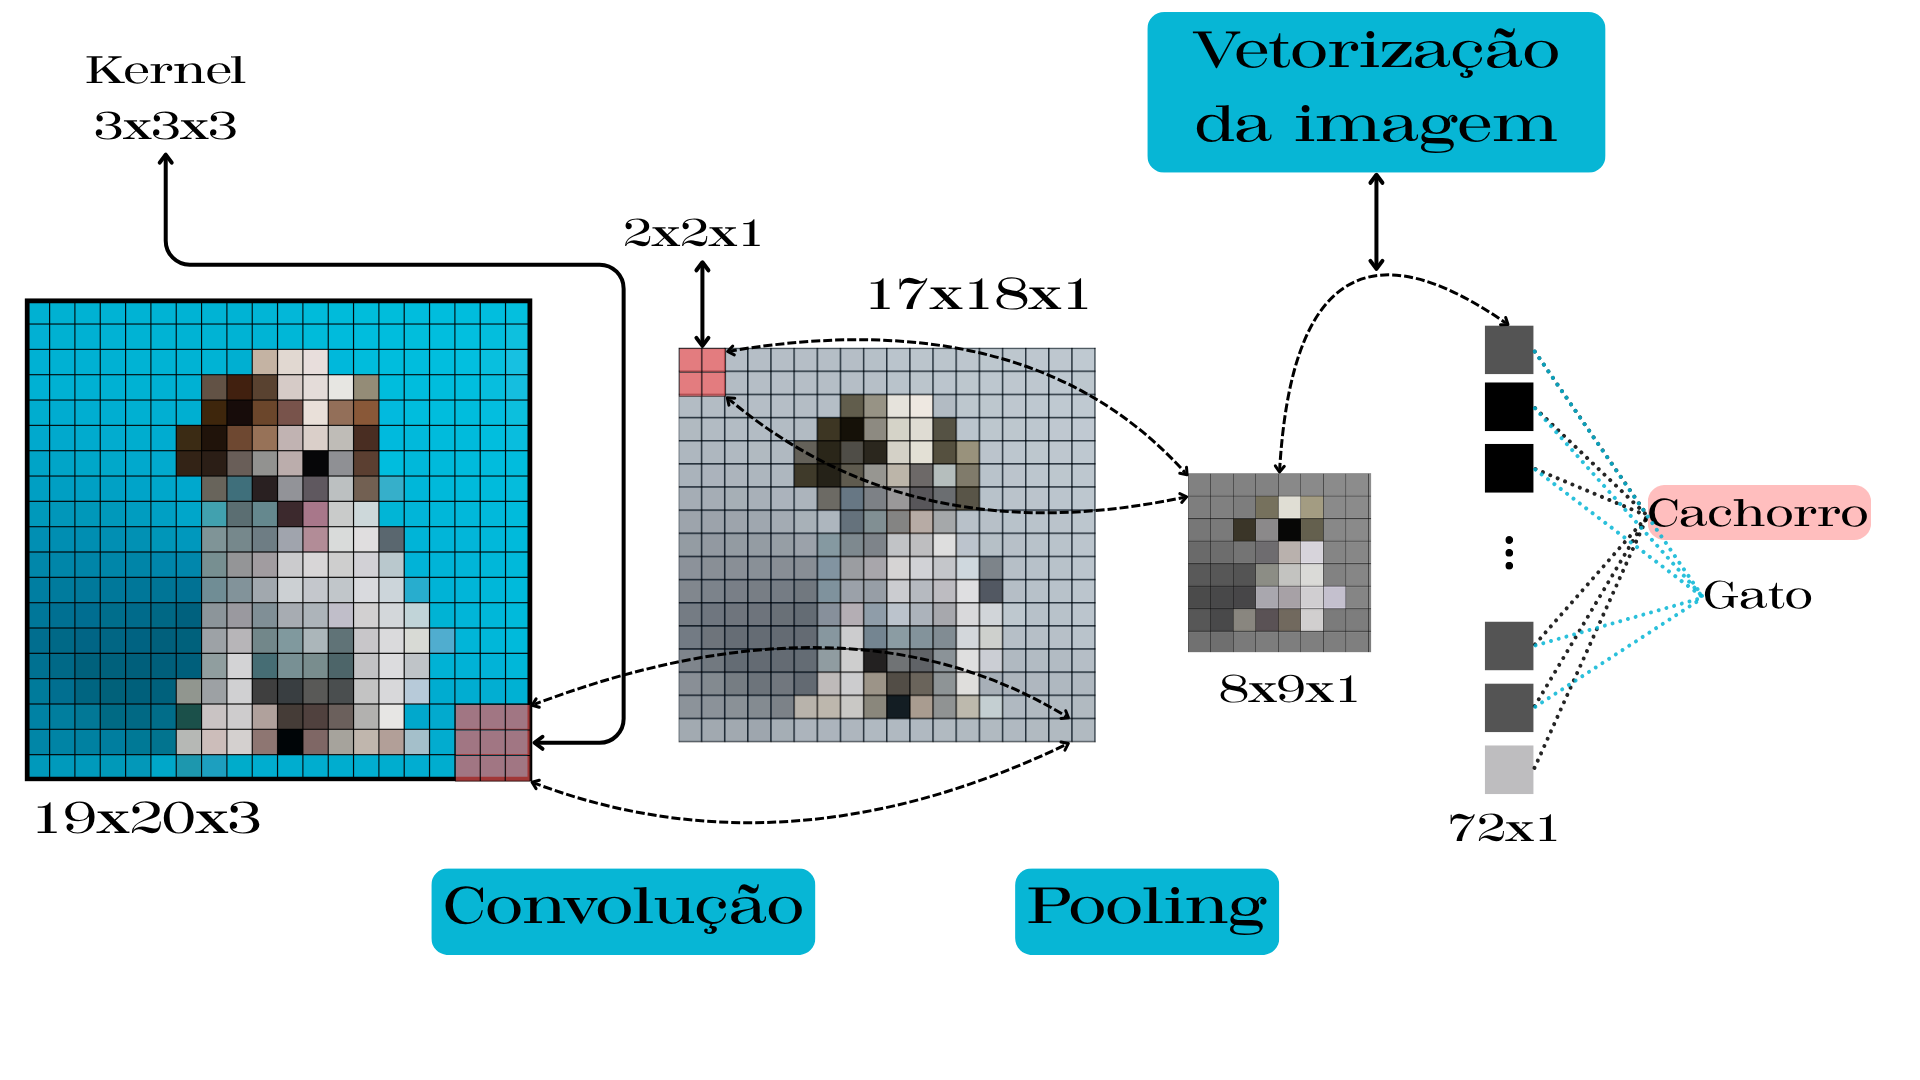
\includegraphics[width=0.7\linewidth]{figures/cnn.png}
    \caption*{\footnotesize Fonte: Elaboração do Autor.}
    \label{cnn}
\end{figure}


\subsection{Convolução Transposta}
A convolução transposta\footnote{O nome sugere uma operação inversa à convolução, entretanto não é isso que acontece. Esse nome provavelmente veio da ideia de ``inverter" a operação de convolução no sentido de expandir as dimensões espaciais da entrada e não diminuir.}, também conhecida como deconvolução, é uma operação utilizada em redes neurais convolucionais para aumentar as dimensões espaciais (largura e altura) dos mapas de características. Essa operação é frequentemente empregada em tarefas de geração de imagens, em que o objetivo é reconstruir imagens a partir de representações compactas. A convolução transposta funciona de maneira inversa à convolução válida. Enquanto a convolução reduz as dimensões espaciais da imagem de entrada, a convolução transposta expande essas dimensões. Isso é alcançado gerando uma saída com dimensões calculadas da seguinte forma:
\begin{equation}
    \begin{split}
    \label{largura_deconv}
    w_{out} = (w_{in} - 1) \cdot s_w - 2w_{pad} + w_{kernel},\\
    h_{out} = (h_{in} - 1) \cdot s_h - 2h_{pad} + h_{kernel},
    \end{split}
\end{equation}
em que $w_{in}$ e $h_{in}$ são a largura e a altura da imagem de entrada, $s_w$ e $s_h$ são os valores do \textit{stride} na largura e na altura, $w_{pad}$ e $h_{pad}$ são a quantidade de pixels adicionados como \textit{padding} na largura e na altura (geralmento os valores para o \textit{padding} são zero), e $w_{kernel}$ e $h_{kernel}$ são a largura e a altura do \textit{kernel}, respectivamente. Cada entrada da imagem de saída é calculada como uma soma ponderada dos valores da imagem de entrada multiplicados pelos pesos do \textit{kernel}. A convolução transposta pode ser implementada utilizando o seguinte Algoritmo \ref{alg:deconv}.
\begin{algorithm}[htpb]
\caption{Convolução Transposta}
\label{alg:deconv}
\KwIn{$X$ (matriz de entrada), $W$ (\textit{kernel}), $s_w$ (\textit{stride} na largura), $s_h$ (\textit{stride} na altura), $w_{pad}$ (\textit{padding} na largura), $h_{pad}$ (\textit{padding} na altura)}
\KwOut{$Y$ (matriz de saída)}
$w_{out} \gets (w_{in} - 1) \cdot s_w - 2w_{pad} + w_{kernel}$\;
$h_{out} \gets (h_{in} - 1) \cdot s_h - 2h_{pad} + h_{kernel}$\;
$Y \gets$ matriz de zeros de tamanho $w_{out} \times h_{out}$\;
\For{$i \gets 0$ \KwTo $w_{in}-1$}{
    \For{$j \gets 0$ \KwTo $h_{in}-1$}{
        \For{$m \gets 0$ \KwTo $w_{kernel}-1$}{
            \For{$n \gets 0$ \KwTo $h_{kernel}-1$}{
                $Y[i \cdot s_w + m - w_{pad}][j \cdot s_h + n - h_{pad}] +=  X[i][j] \cdot W[m][n]$\;
            }
        }
    }
}
\end{algorithm}

A Figura \ref{fig:conTrans} exemplifica a operação de convolução transposta, em que uma matriz de entrada $X$ (matriz $2\times2$) é operada com um \textit{kernel} $W$ (matriz $2\times2$) para produzir a saída $Y$ (matriz $3\times3$). 
\begin{figure}[htpb]
    \centering
    \caption{Exemplo da operação de convolução transposta.}
    
\includegraphics[width=0.7\linewidth]{deconv.png}
    \caption*{\footnotesize Fonte: Elaboração do Autor.}
    \label{fig:conTrans}
\end{figure}

\
\section{U-net: Rede Convolucional para Segmentação de Imagens}
\label{sec:unet}
Modificando a arquitetura tradicional de uma CNN, é possível obter variadas redes neurias com objetivos específicos. O uso típico de redes convolucionais ocorre em tarefas de classificação, em que o objetivo é atribuir uma etiqueta a uma imagem inteira. No entanto, em muitas tarefas visuais, especialmente no processamento de imagens biomédicas, a saída desejada deve incluir informações espaciais detalhadas, como a localização precisa de estruturas dentro da imagem. Para atender a essa necessidade, foi proposta a arquitetura U-Net \cite{Ronneberger2015UNet}, que é uma rede neural convolucional projetada para segmentação de imagens. A U-Net é composta por uma parte de contração (\textit{encoder}, composta por camadas de convolução e \textit{pooling}) e uma parte de expansão (\textit{decoder}, composta por camadas de convolução transposta), formando uma estrutura em forma de U (origem do nome U-Net). O \textit{encoder} é responsável por extrair características da imagem de entrada, enquanto o \textit{decoder} reconstrói a imagem, utilizando as características extraídas pelo \textit{encoder}. A arquitetura U-Net é especialmente eficaz em tarefas de segmentação semântica, em que o objetivo é classificar cada pixel da imagem em uma categoria específica, permitindo a identificação precisa de objetos e estruturas dentro da imagem. O Exemplo \ref{ex:unet} apresenta uma simplificação visual do funcionamento da U-Net antes de ser introduzido os detalhes da arquitetura completa.

\begin{exemplo}
    \label{ex:unet}
    Seja uma imagem de entrada normalizada $X$ de dimensões $5\times 5$ e uma resposta desejada $Y$ de dimensões $5\times 5$, a Figura \ref{unet-simples} apresenta as duas imagens, em que $1$ representa a cor mais brilhante e $0$ representa o fundo branco.
    
\begin{figure}[htpb]
    \centering
    \caption{Imagem de entrada $X$ e resposta desejada $Y$.}
    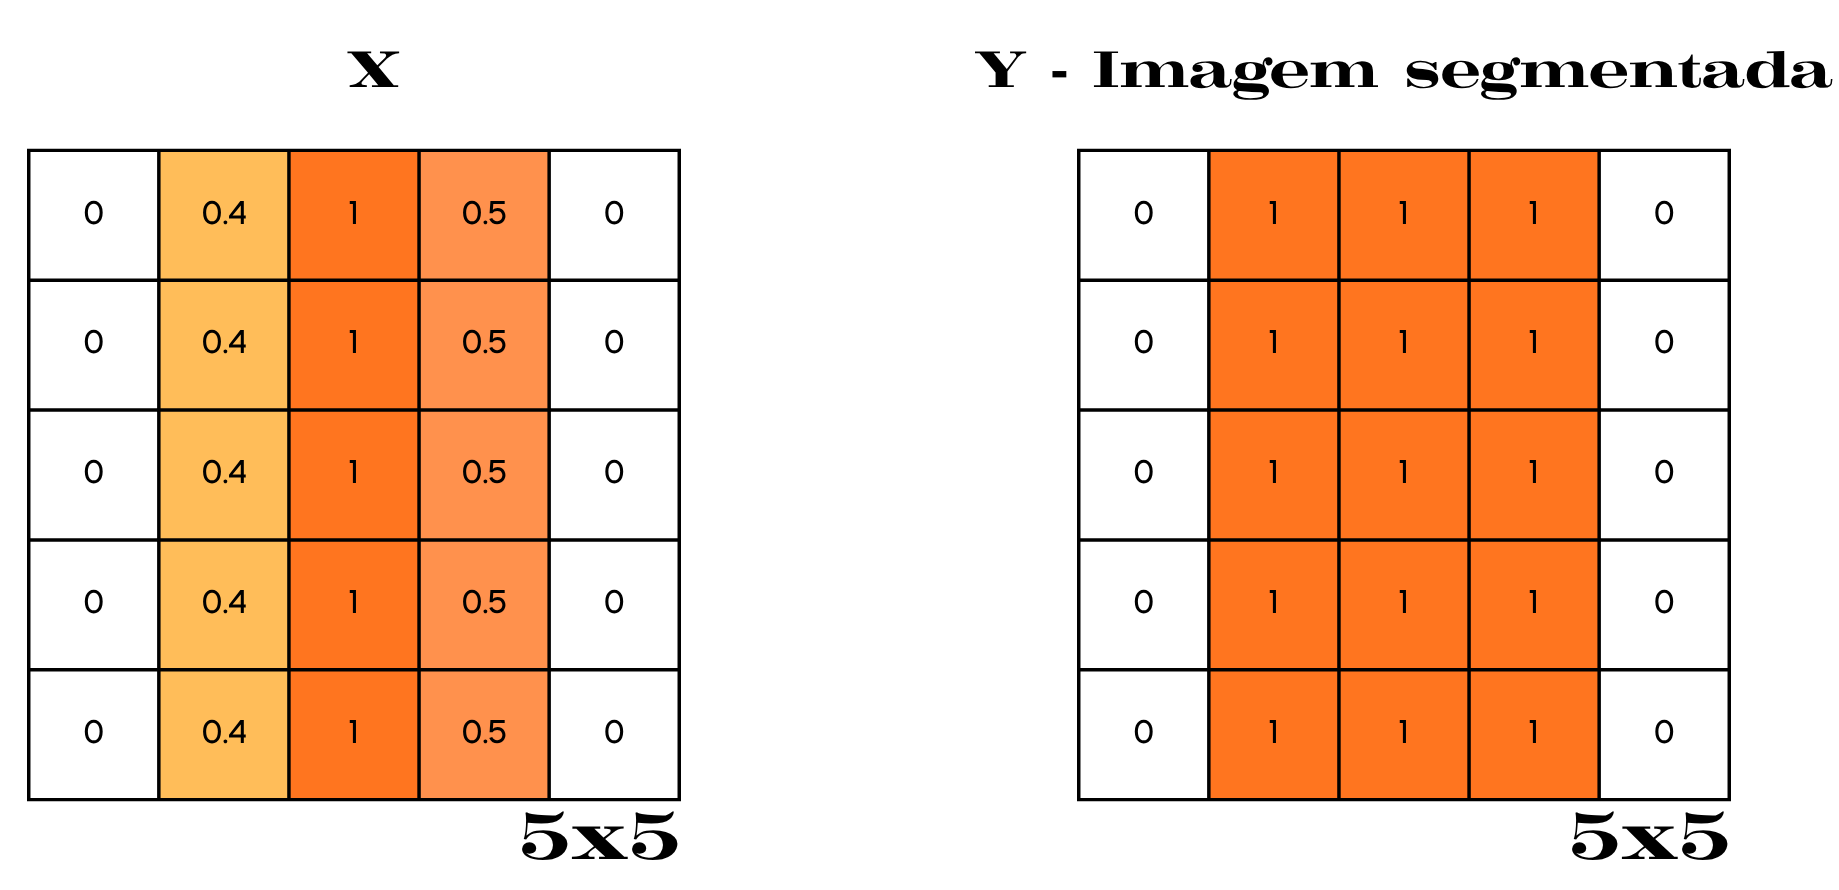
\includegraphics[width=0.7\linewidth]{figures/unetimgs/ex_fig1.png}
    \caption*{\footnotesize Fonte: Elaboração do Autor.}
    \label{unet-simples}
\end{figure}
Na imagem de saída esperada, pode-se entender os valores de pixel iguais a $1$ como regiões de interesse e os valores iguais a $0$ como fundo. O primeiro passo para gerar a imagem de saída é aplicar a operação de convolução na imagem de entrada $X$ utilizando um \textit{kernel} que neste exemplo é uma matriz $2\times 2$, como mostra a Figura\ref{ex:unet_img2}.
\begin{figure}[H]
    \centering
    \caption{Aplicação de um \textit{kernel} de convolução na imagem de entrada $X$. O resultado da convolução é um mapa de características que destaca as regiões de interesse na imagem.}
    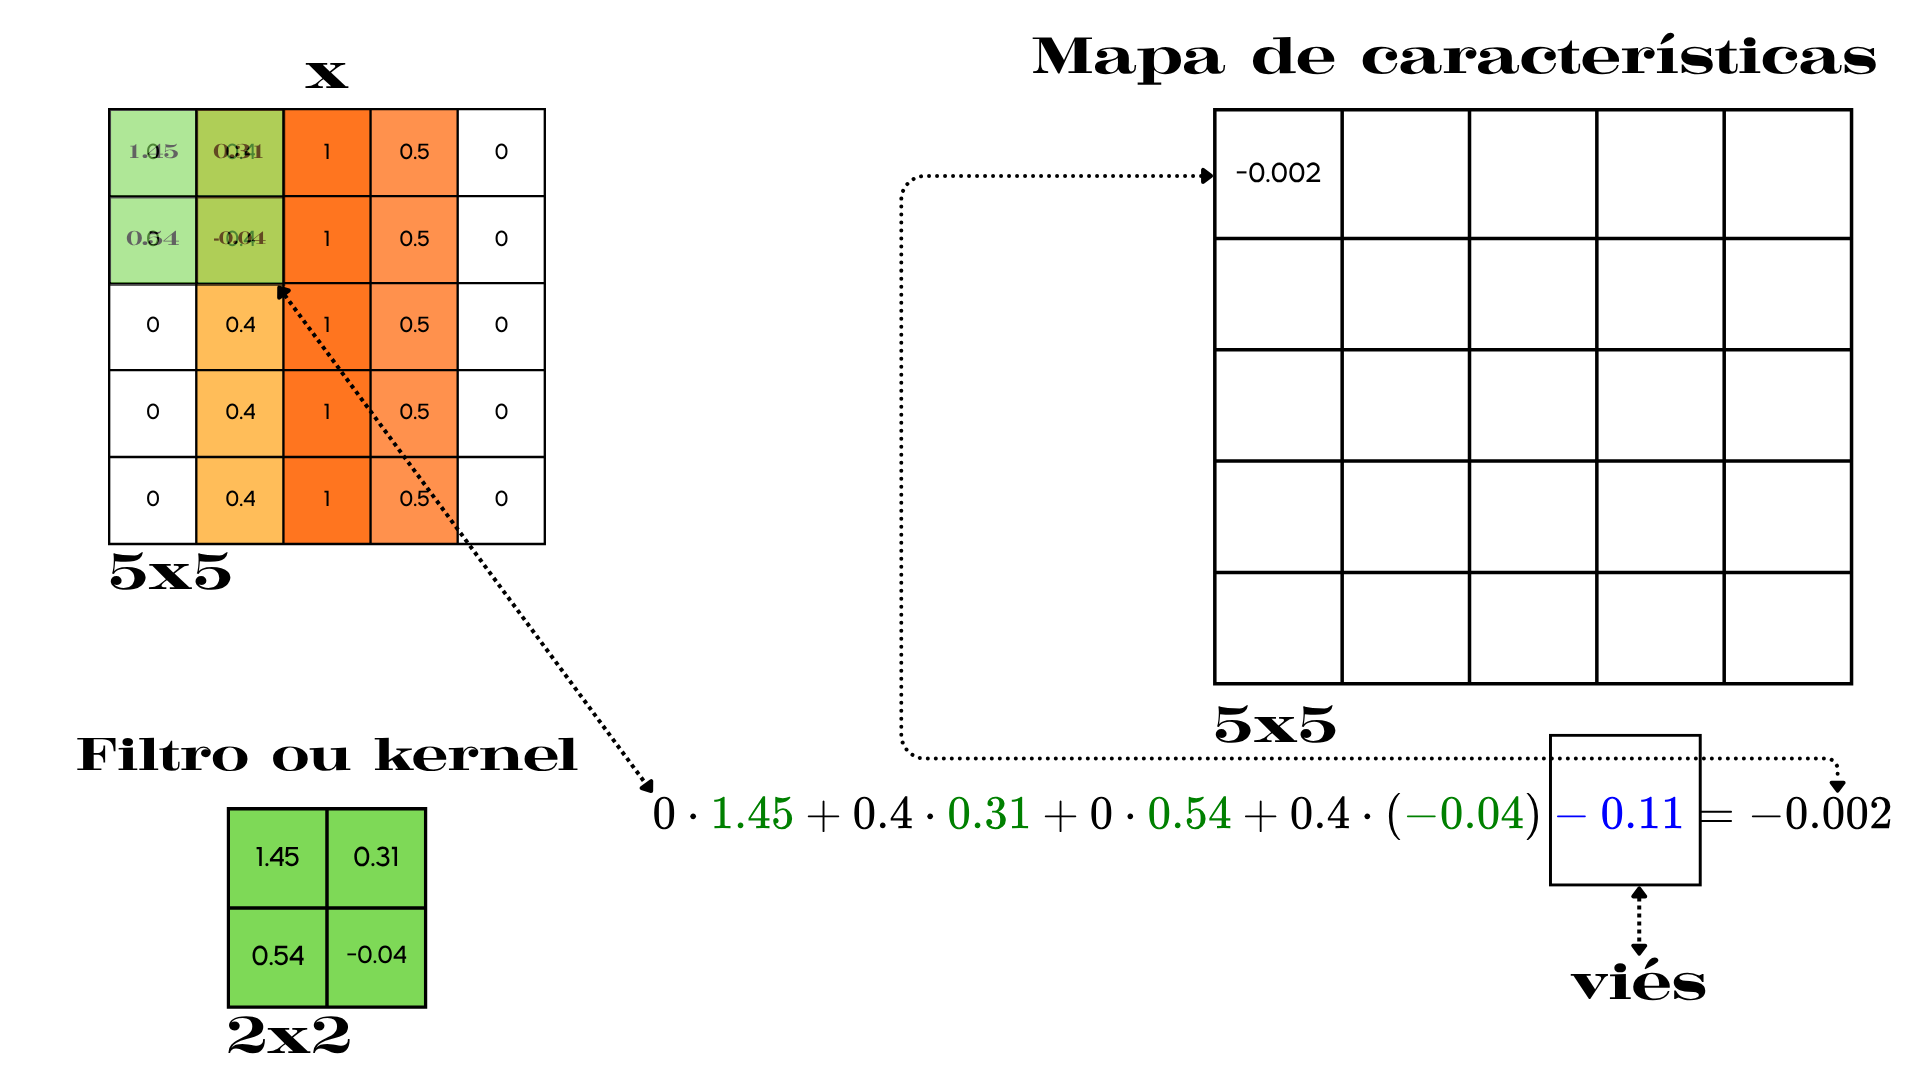
\includegraphics[width=0.8\linewidth]{figures/unetimgs/ex_fig2.png}
    \caption*{\footnotesize Fonte: Elaboração do Autor.}
    \label{ex:unet_img2}
\end{figure}
Os valores do \textit{kernel} e do viés que apareceram neste exemplo já foram otimizados para destacar as regiões de interesse na imagem. Para que o mapa de características resultante da convolução tenha as mesmas dimensões da imagem de entrada, é necessário aplicar a técnica de padding, adicionando uma borda de zeros ao redor da imagem de entrada $X$, como mostra a Figura \ref{ex:unet_img3}.
\begin{figure}[H]
    \centering
    \caption{Aplicação de padding na imagem de entrada $X$ para preservar suas dimensões durante a operação de convolução.}
    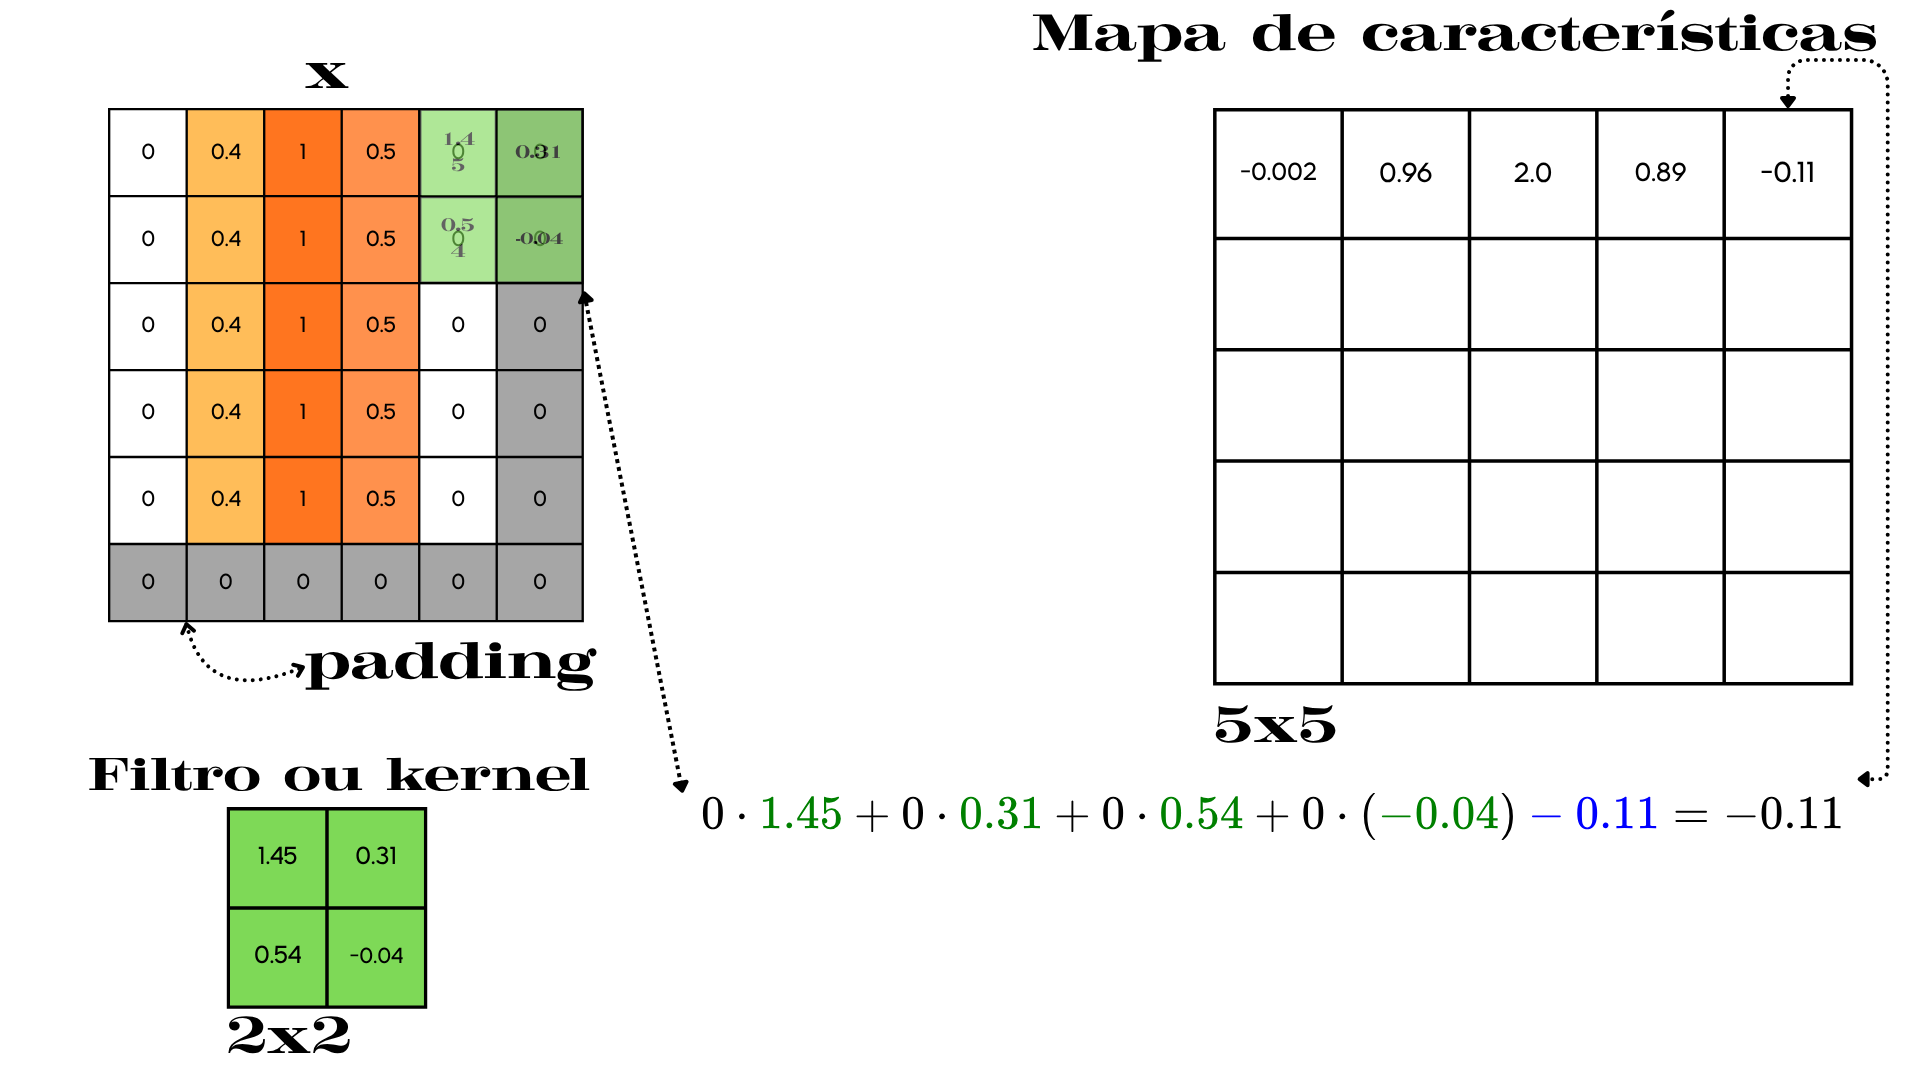
\includegraphics[width=0.8\linewidth]{figures/unetimgs/ex_fig3.png}
    \caption*{\footnotesize Fonte: Elaboração do Autor.}
    \label{ex:unet_img3}
\end{figure}

Após o \textit{kernel} ser aplicado na imagem de entrada $X$ com o uso de padding, é gerado um mapa de características, entretanto para completar a operação, é necessário aplicar uma função de ativação em cada valor do mapa, como mostra a Figura \ref{ex:unet_img4}. A função de ativação utilizada é a função \textit{ReLU}, vista na Equação \ref{eq:relu}.
\begin{figure}[htpb]
    \centering
    \caption{Aplicação da função de ativação ReLU no mapa de características resultante da convolução.}
    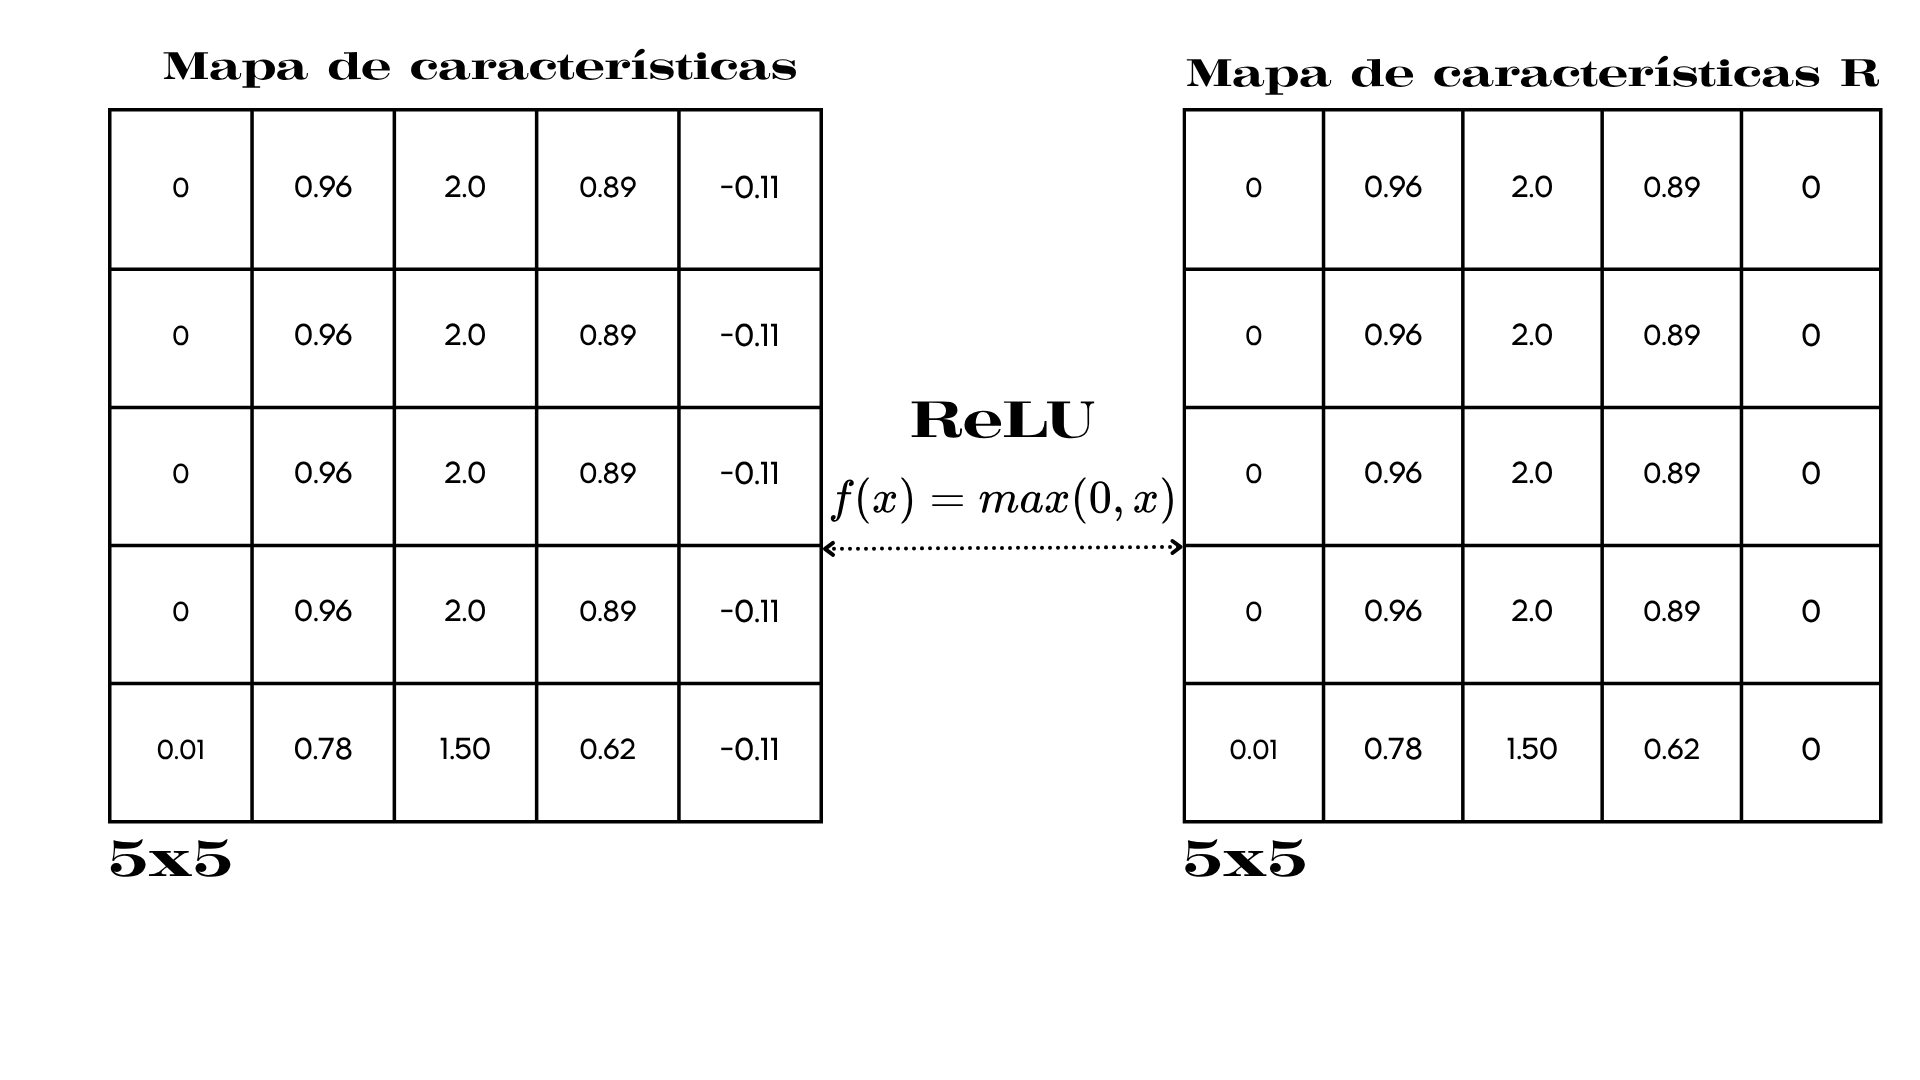
\includegraphics[width=0.9\linewidth]{figures/unetimgs/ex_fig4.png}
    \caption*{\footnotesize Fonte: Elaboração do Autor.}
    \label{ex:unet_img4}
\end{figure}

O mapa de características resultante da aplicação da função de ativação é então processado por uma camada de \textit{Max pooling} de dimensões $2\times 2$ e \textit{stride} 2, que reduz suas dimensões espaciais pela metade, como mostra a Figura \ref{ex:unet_img5}.
\begin{figure}[H]
    \centering
    \caption{Aplicação de uma camada de \textit{Max pooling} no mapa de características resultante.}
    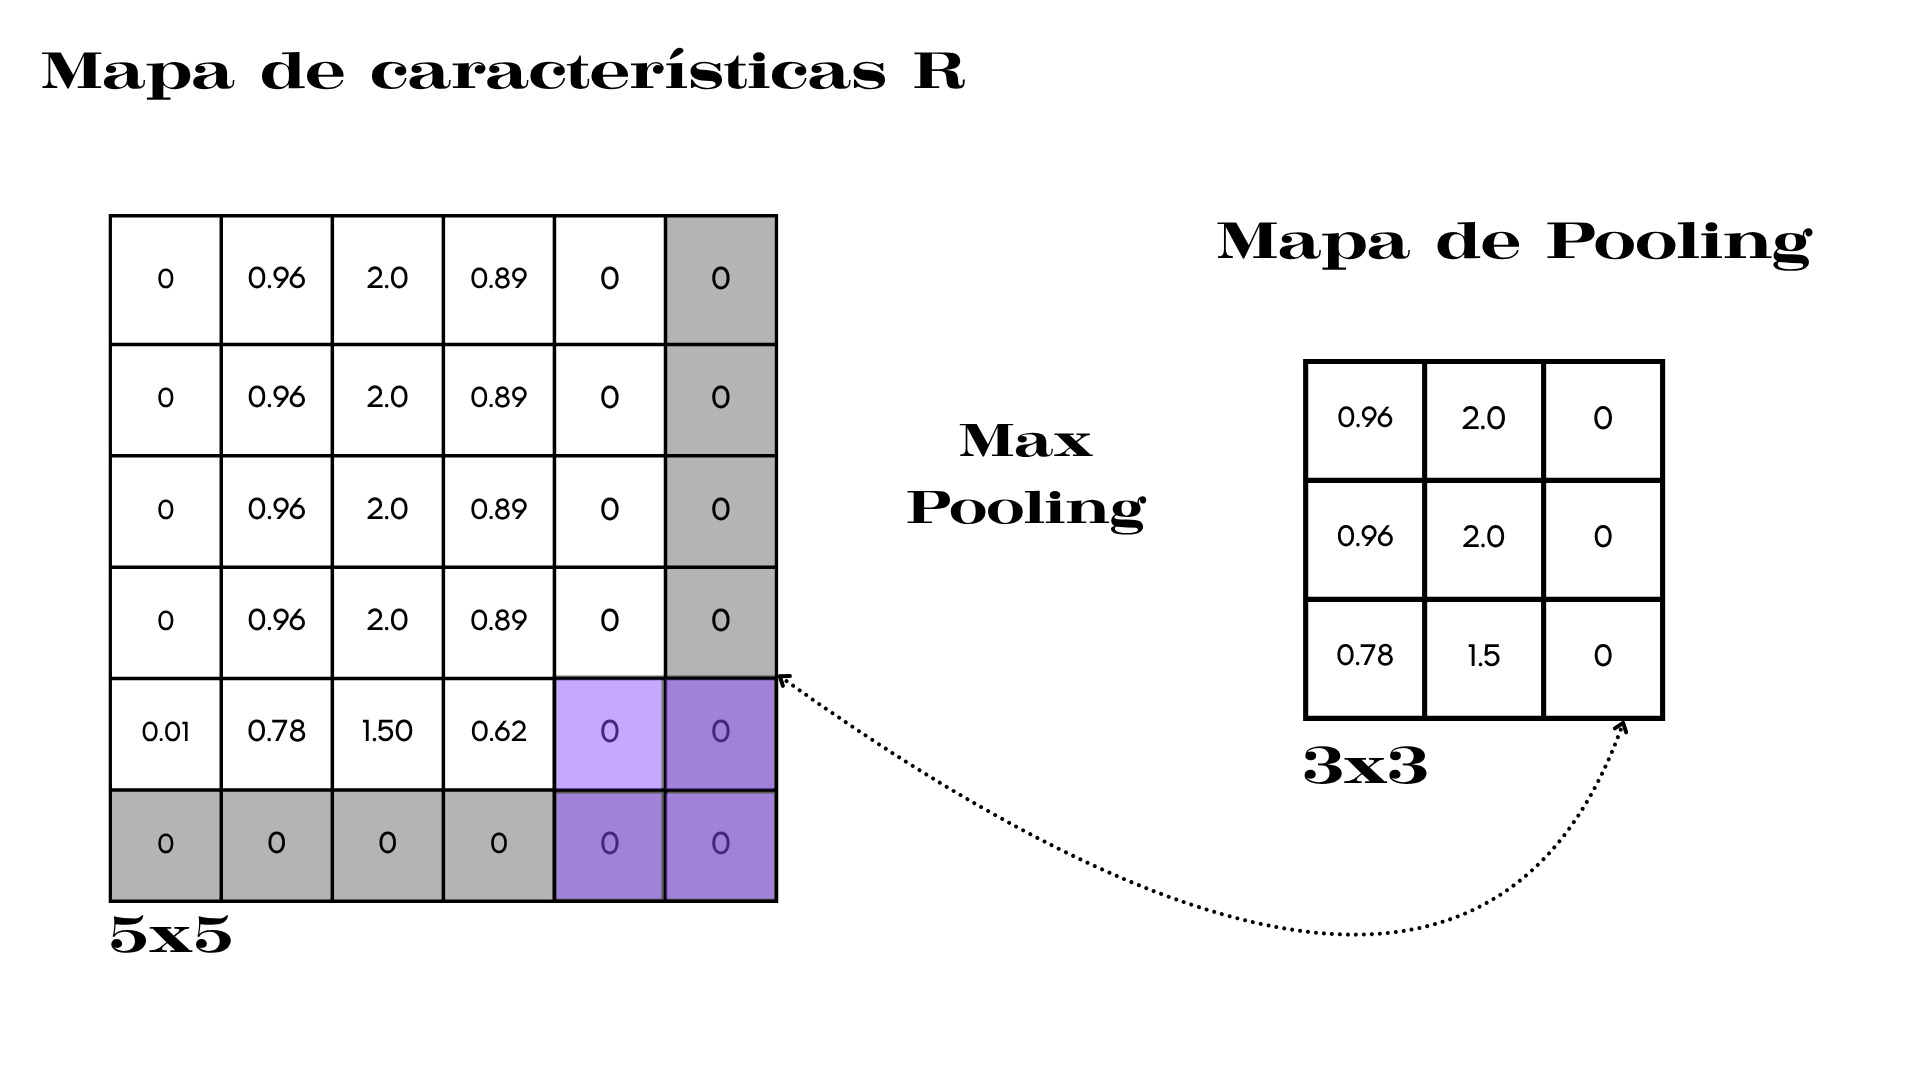
\includegraphics[width=0.75\linewidth]{figures/unetimgs/ex_fig5.png}
    \caption*{\footnotesize Fonte: Elaboração do Autor.}
    \label{ex:unet_img5}
\end{figure}

Com o mapa de pooling gerado, para voltar as dimensões originais da imagem de entrada, é necessário aplicar a operação de convolução transposta, utilizando um \textit{kernel} de dimensões $2\times 2$, como mostra a Figura \ref{ex:unet_img6}.
\begin{figure}[H]
    \centering
    \caption{Aplicação da operação de convolução transposta no mapa de pooling para expandir suas dimensões espaciais e voltar às dimensões originais da imagem de entrada.}
    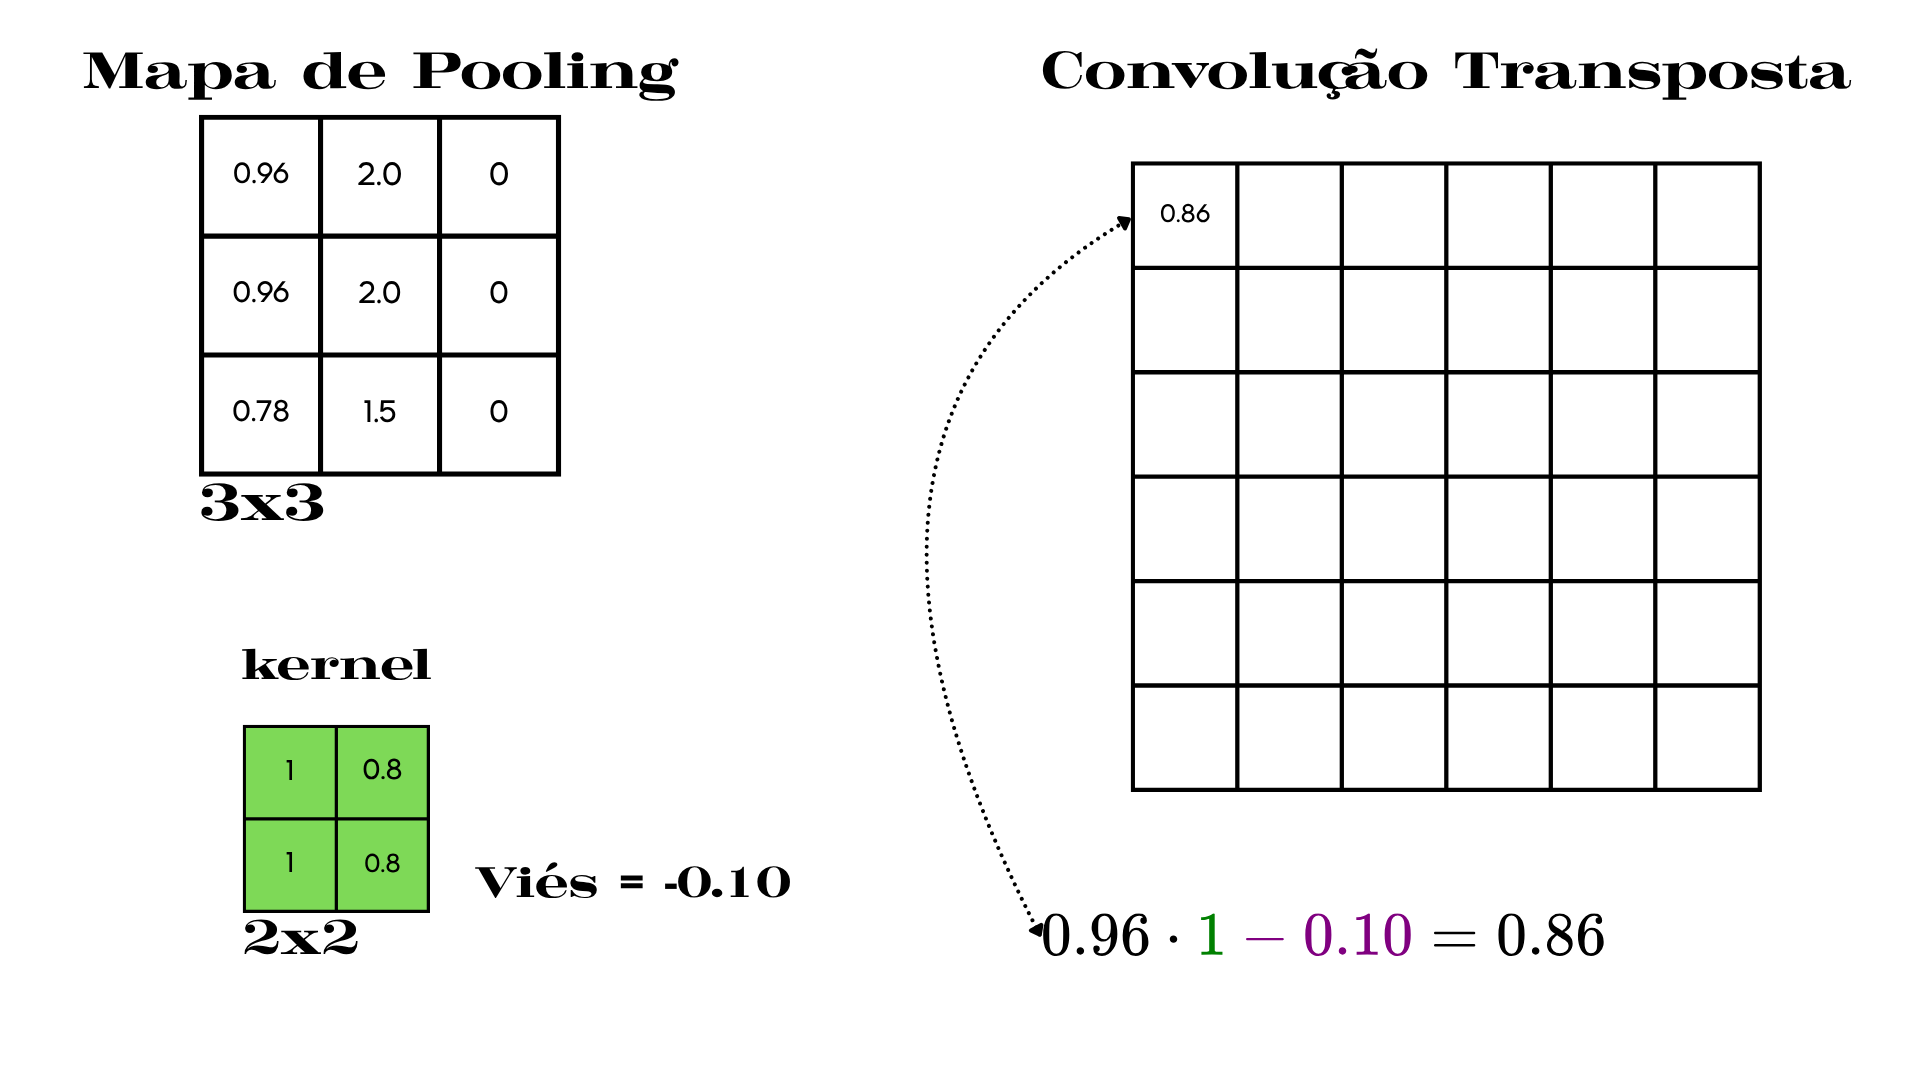
\includegraphics[width=0.8\linewidth]{figures/unetimgs/ex_fig6.png}
    \caption*{\footnotesize Fonte: Elaboração do Autor.}
    \label{ex:unet_img6}
\end{figure}
O nome U-Net vem da forma em U da arquitetura, em que o encoder diminui as dimensões espaciais da imagem de entrada, enquanto o decoder as expande, formando uma estrutura simétrica, como mostra a Figura \ref{ex:unet_img7}.
\begin{figure}[H]
    \centering
    \caption{Estrutura em forma de U da arquitetura U-Net. O encoder é responsável por extrair características da imagem de entrada, enquanto o decoder reconstrói a imagem, utilizando as características extraídas pelo encoder.}
    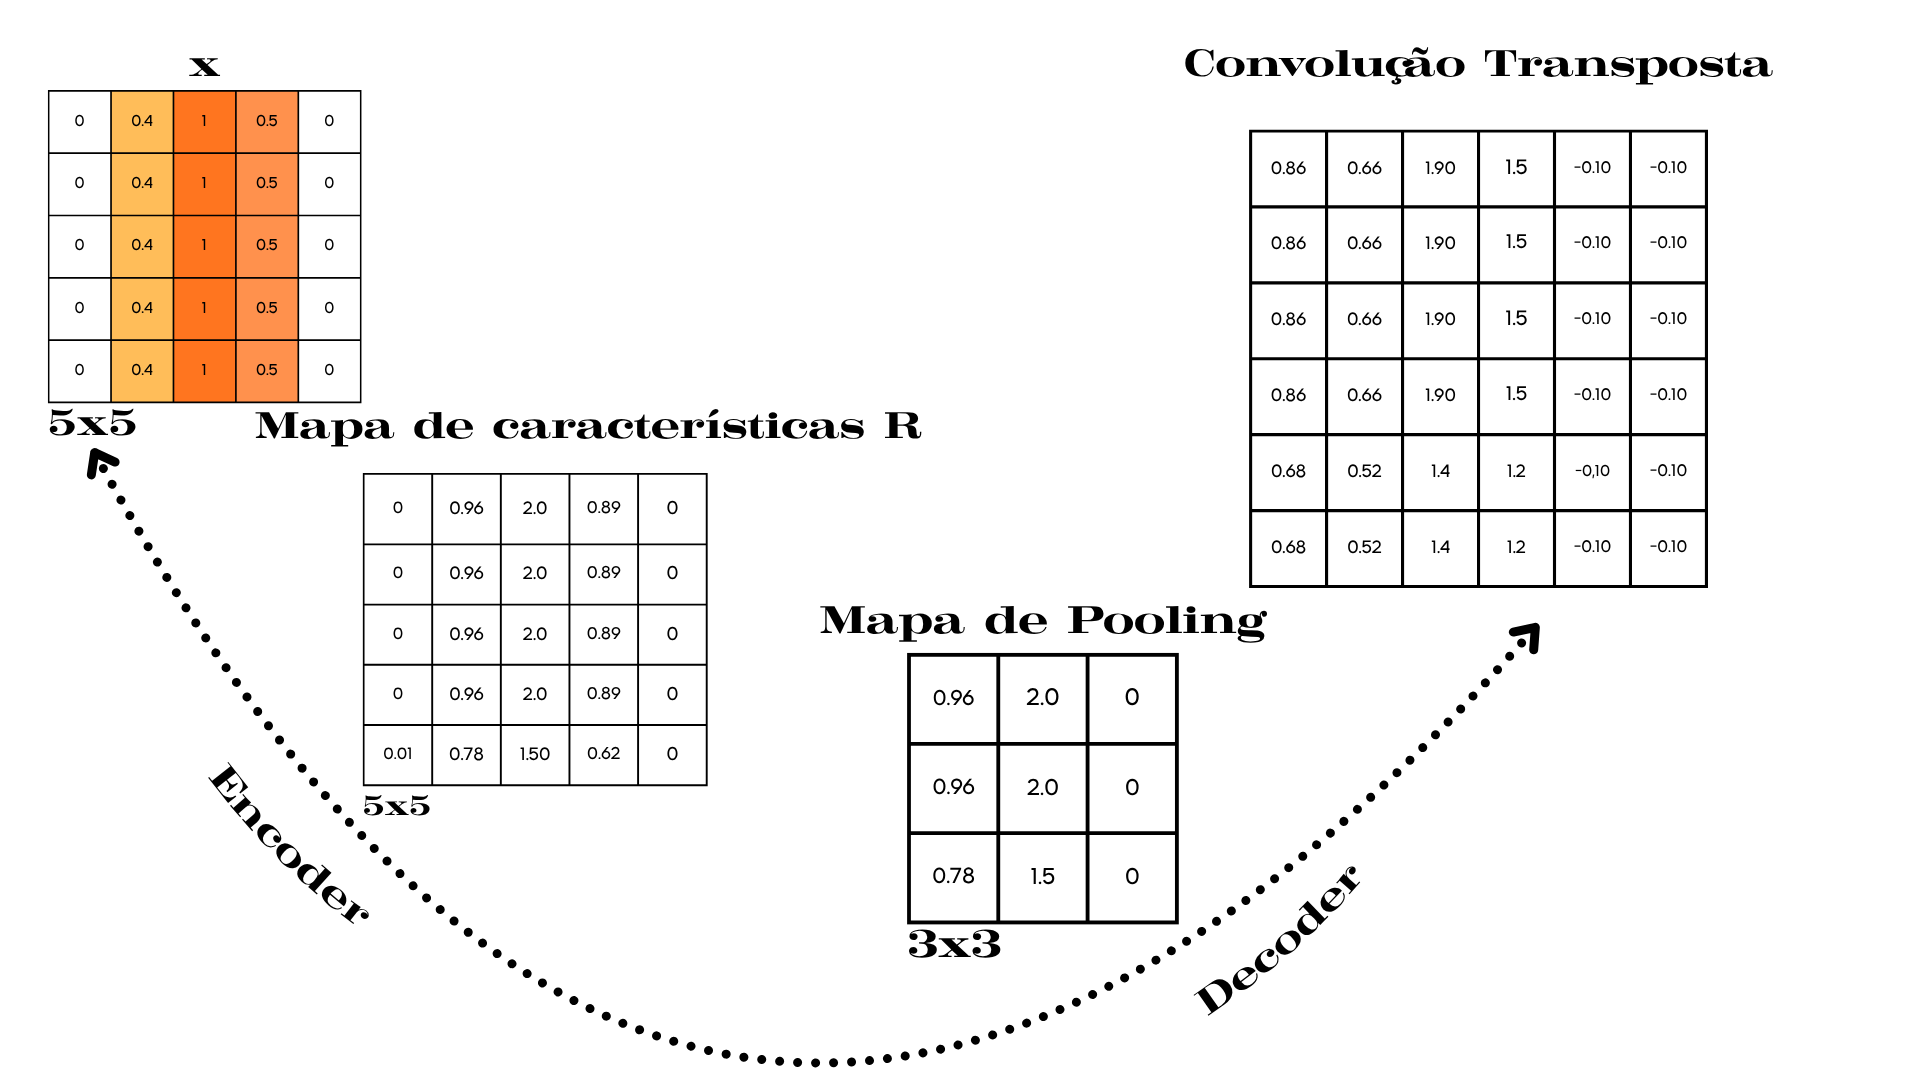
\includegraphics[width=0.8\linewidth]{figures/unetimgs/ex_fig7.png}
    \caption*{\footnotesize Fonte: Elaboração do Autor.}
    \label{ex:unet_img7}
\end{figure}
A característica mais importante da arquitetura U-Net é a presença de conexões de atalho (\textit{skip connections}) entre as camadas correspondentes do encoder e do decoder, presente na Figura \ref{ex:unet_img8}. 
\begin{figure}[htpb]
    \centering
    \caption{Exemplo de conexões de atalho (\textit{skip connections}) na arquitetura U-Net.}
    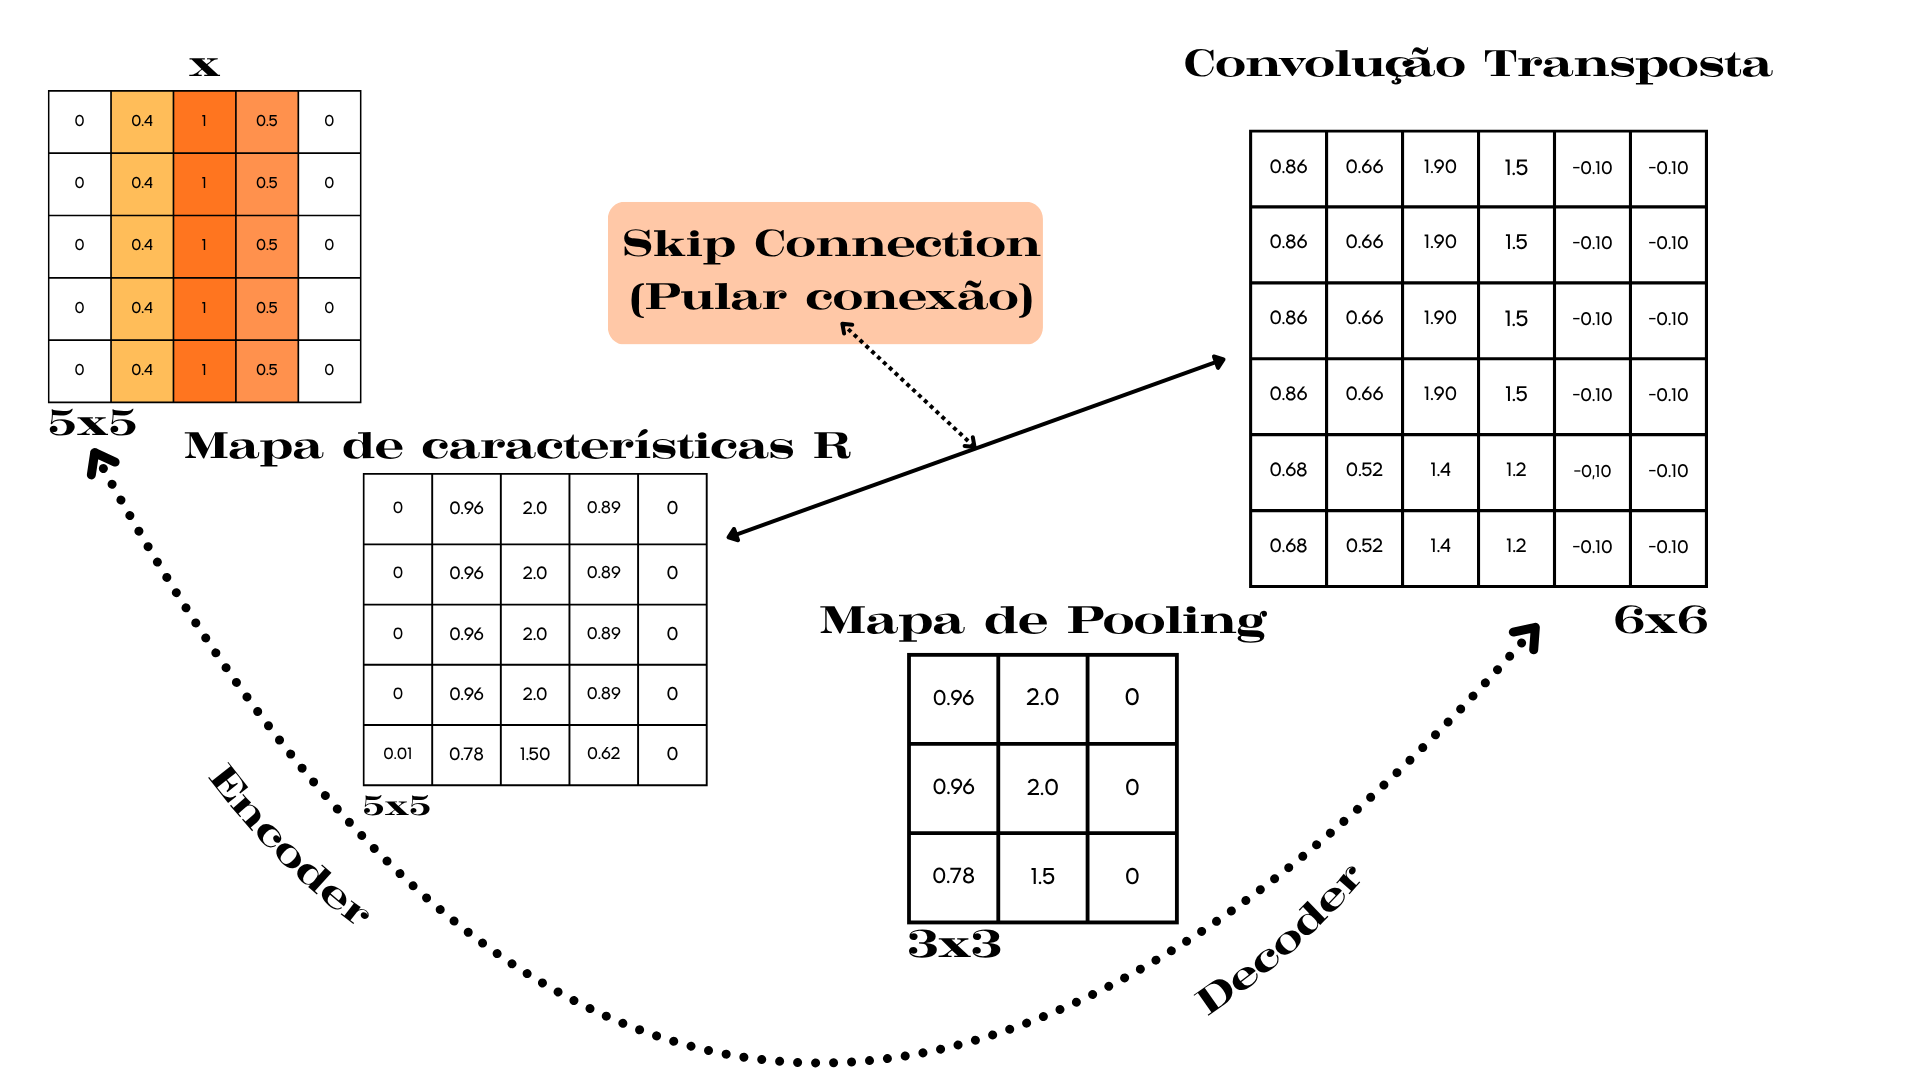
\includegraphics[width=0.8\linewidth]{figures/unetimgs/ex_fig8.png}
    \caption*{\footnotesize Fonte: Elaboração do Autor.}
    \label{ex:unet_img8}
\end{figure}
Essa operação concatena as imagens conrrespondentes, entretanto para que as imagens possam ser concatenadas, é necessário que elas tenham as mesmas dimensões, portanto, é necessário aplicar a técnica de \textit{copy} (copiar) and (e) \textit{crop} (cortar), em que as características extraídas pelo decoder são copiadas e recortadas para se encaixar nas dimensões da camada correspondente no encoder, a sobreposição é feita começando de cima para baixo, da esquerda para a direita, com o vermelho sinalizando a área que será removida após a sobreposição, como mostra a Figura \ref{ex:unet_img9}. 

\begin{figure}[htpb]
    \centering
    \caption{Exemplo de conexões de atalho (\textit{skip connections}) na arquitetura U-Net. As conexões de atalho permitem que as informações de baixo nível, como bordas e texturas, sejam diretamente transferidas do encoder para o decoder, facilitando a reconstrução precisa da imagem segmentada.}
    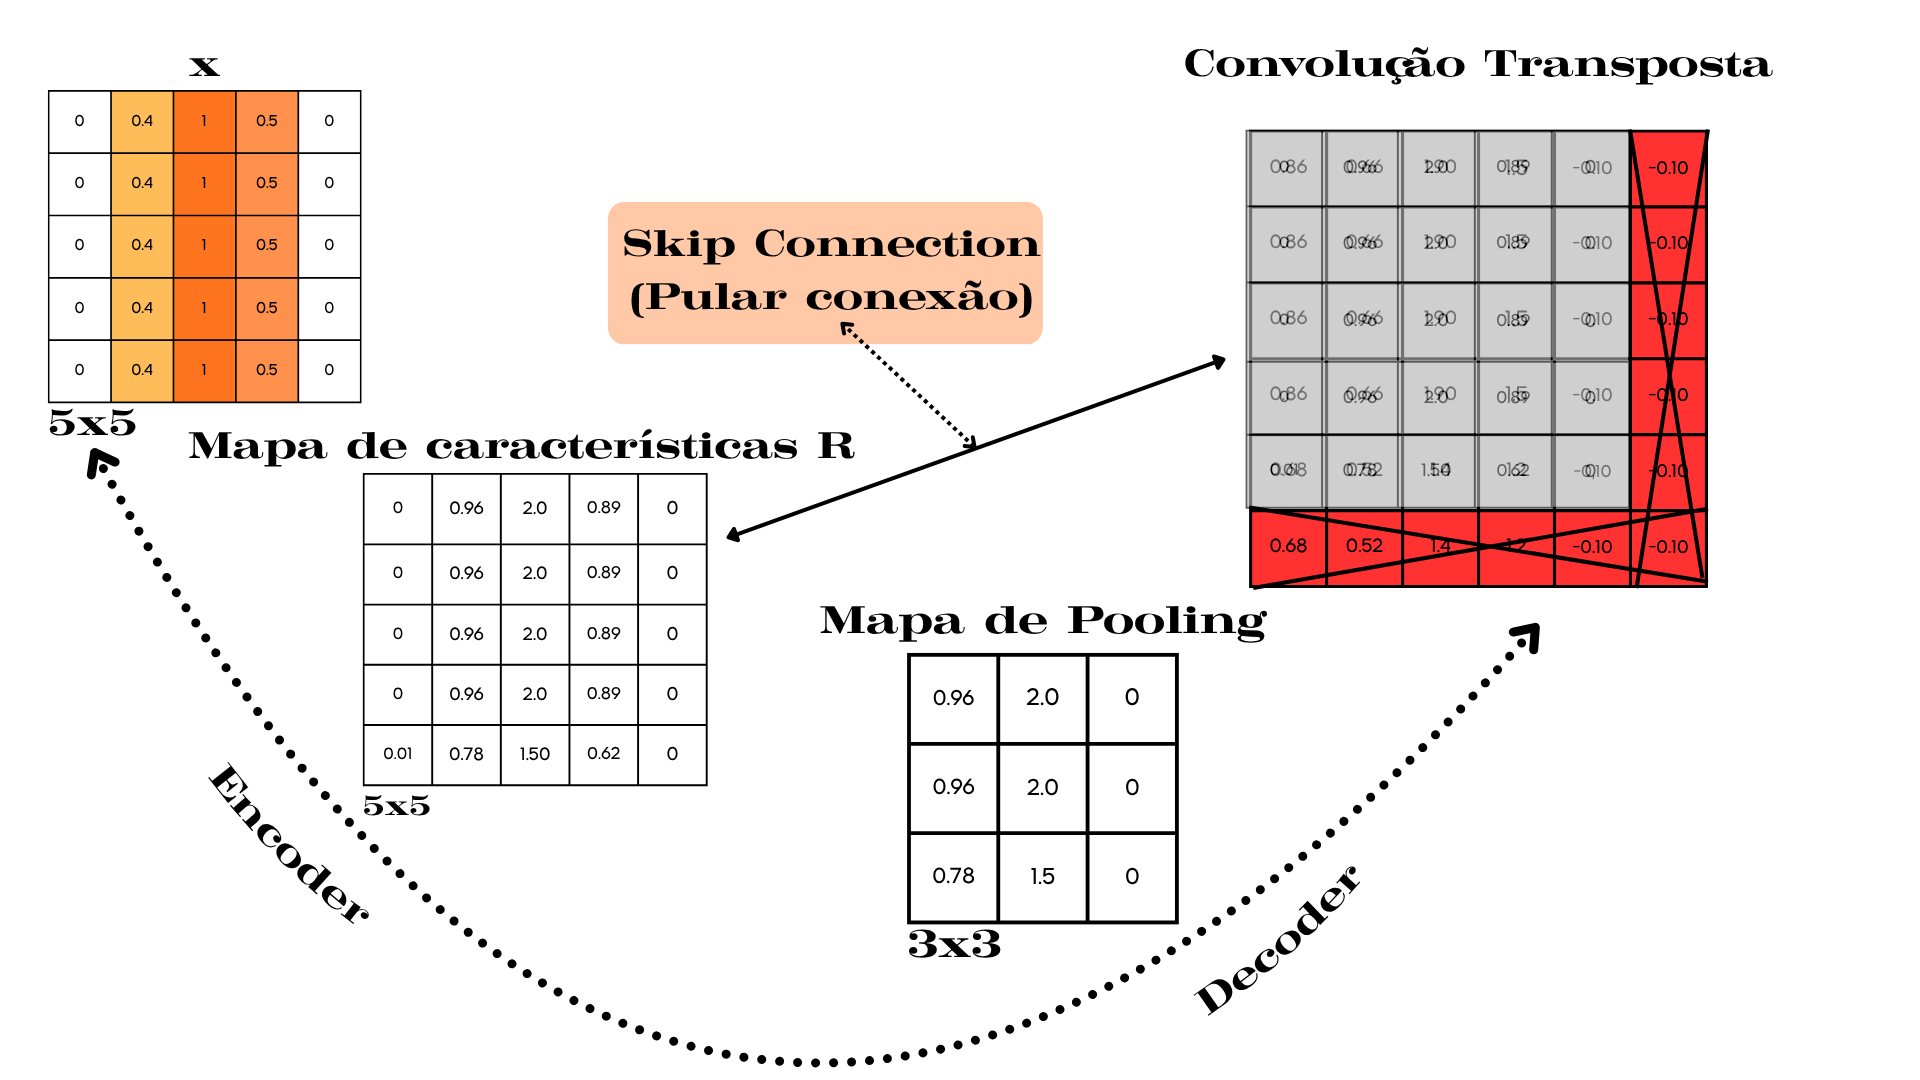
\includegraphics[width=0.9\linewidth]{figures/unetimgs/ex_fig9.png}
    \caption*{\footnotesize Fonte: Elaboração do Autor.}
    \label{ex:unet_img9}
\end{figure}


Dependedo da convolução utilizada, o \textit{ copy and crop} pode ser aplicado a imagem do encoder e caso as imagens tenham mais de um canal, a operação de concatenação leva em consideração apenas a altura e a largura das imagens, ou seja, as imagens precisão ter as mesmas dimensões, os canais de cada imagem são somados no processo, por exemplo:
$$
X_1 = (A,L,C_1) \oplus X_2 =(A,L,C_2) = (A,L,C_1 + C_2) = Y,
$$
em que $A$ é a altura, $L$ é a largura e $C$ é a quantidade de canais de cada imagem e $\oplus$ representa a operação de concatenação ao longo do eixo dos canais. 


Para finalizar a concatenação, é necessário aplicar uma última camada de convolução. Como as imagens estão sobrepostas, por conta da concatenação, o \textit{kernel} fica com dimensões $(1\times 1 \times 2)$, um canal para cada imagem, como mostra a Figura \ref{ex:unet_img10}. No fim da convolução, é necessário aplicar uma função de ativação, neste caso a  \textit{sigmoid logística} vista na Equação \ref{eq:sigmoid}, para gerar a imagem de saída $Y$ com valores entre 0 e 1, representando a probabilidade de cada pixel pertencer à classe segmentada. Neste exemplo, quanto mais próximo de 1, mais brilhante é o pixel, indicando uma maior probabilidade de não estar no plano de fundo da imagem, enquanto valores próximos de 0 indicam uma maior probabilidade de pertecerem ao plano de fundo. 
\begin{figure}[H]
    \centering
    \caption{Aplicação de uma última camada de convolução para gerar a imagem de saída $Y$. O \textit{kernel} utilizado tem dimensões $(1\times 1 \times 2)$, um canal para cada imagem resultante da concatenação.}
    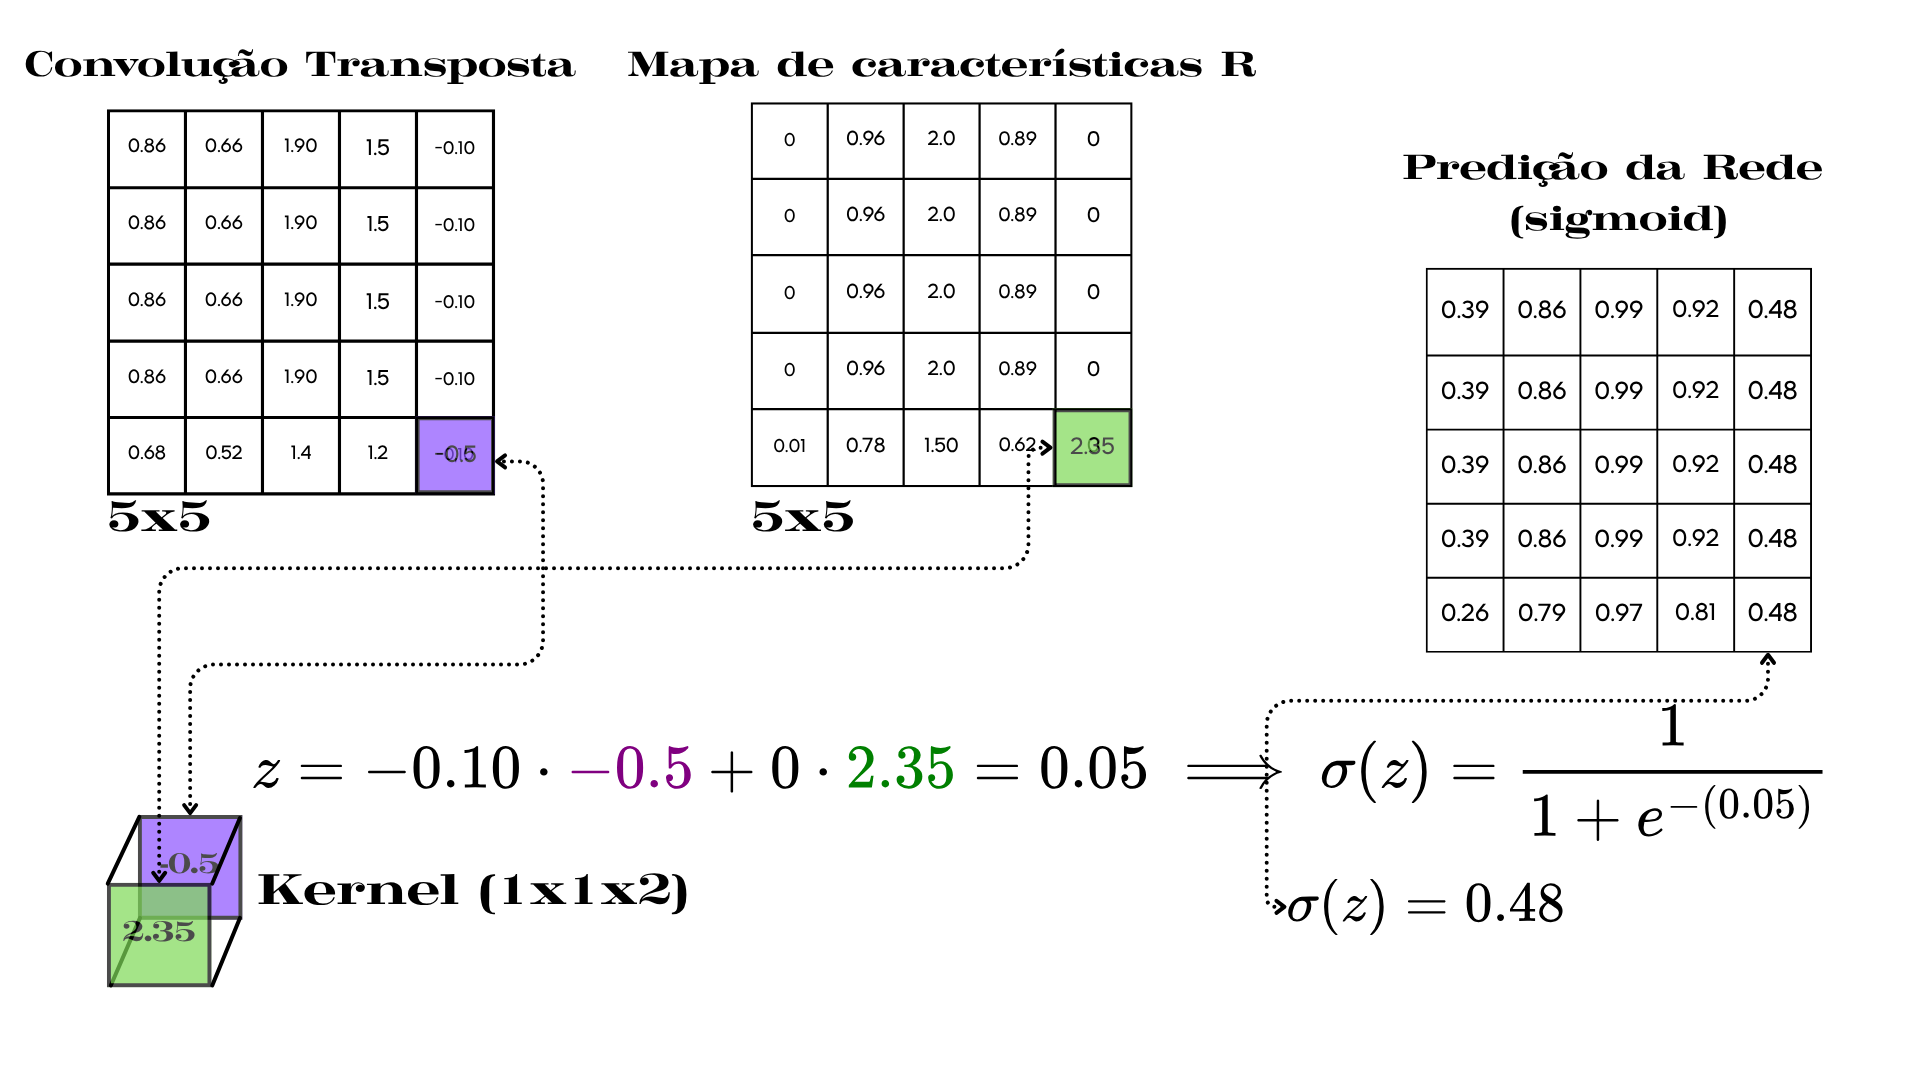
\includegraphics[width=0.8\linewidth]{figures/unetimgs/ex_fig10.png}
    \caption*{\footnotesize Fonte: Elaboração do Autor.}
    \label{ex:unet_img10}
\end{figure}
Por fim, como a imagem segmentada, presente na Figura \ref{unet-simples}, tem valores $0$ e $1$, é necessário aplicar um limiar (\textit{threshold}) na imagem gerada após a aplicação da função sigmoid. Como mostra a Figura \ref{ex:unet_img11}.
\begin{figure}[H]
    \centering
    \caption{Aplicação de um limiar (\textit{threshold}) para gerar a imagem binária final. A imagem segmentada resultante da aplicação da função de ativação sigmoid tem valores entre 0 e 1, representando a probabilidade de cada pixel pertencer à classe segmentada. O limiar é aplicado para converter esses valores em uma imagem binária, onde pixels com valores acima do limiar são classificados como pertencentes à classe segmentada (1), enquanto pixels com valores abaixo do limiar são classificados como pertencentes ao plano de fundo (0).}
    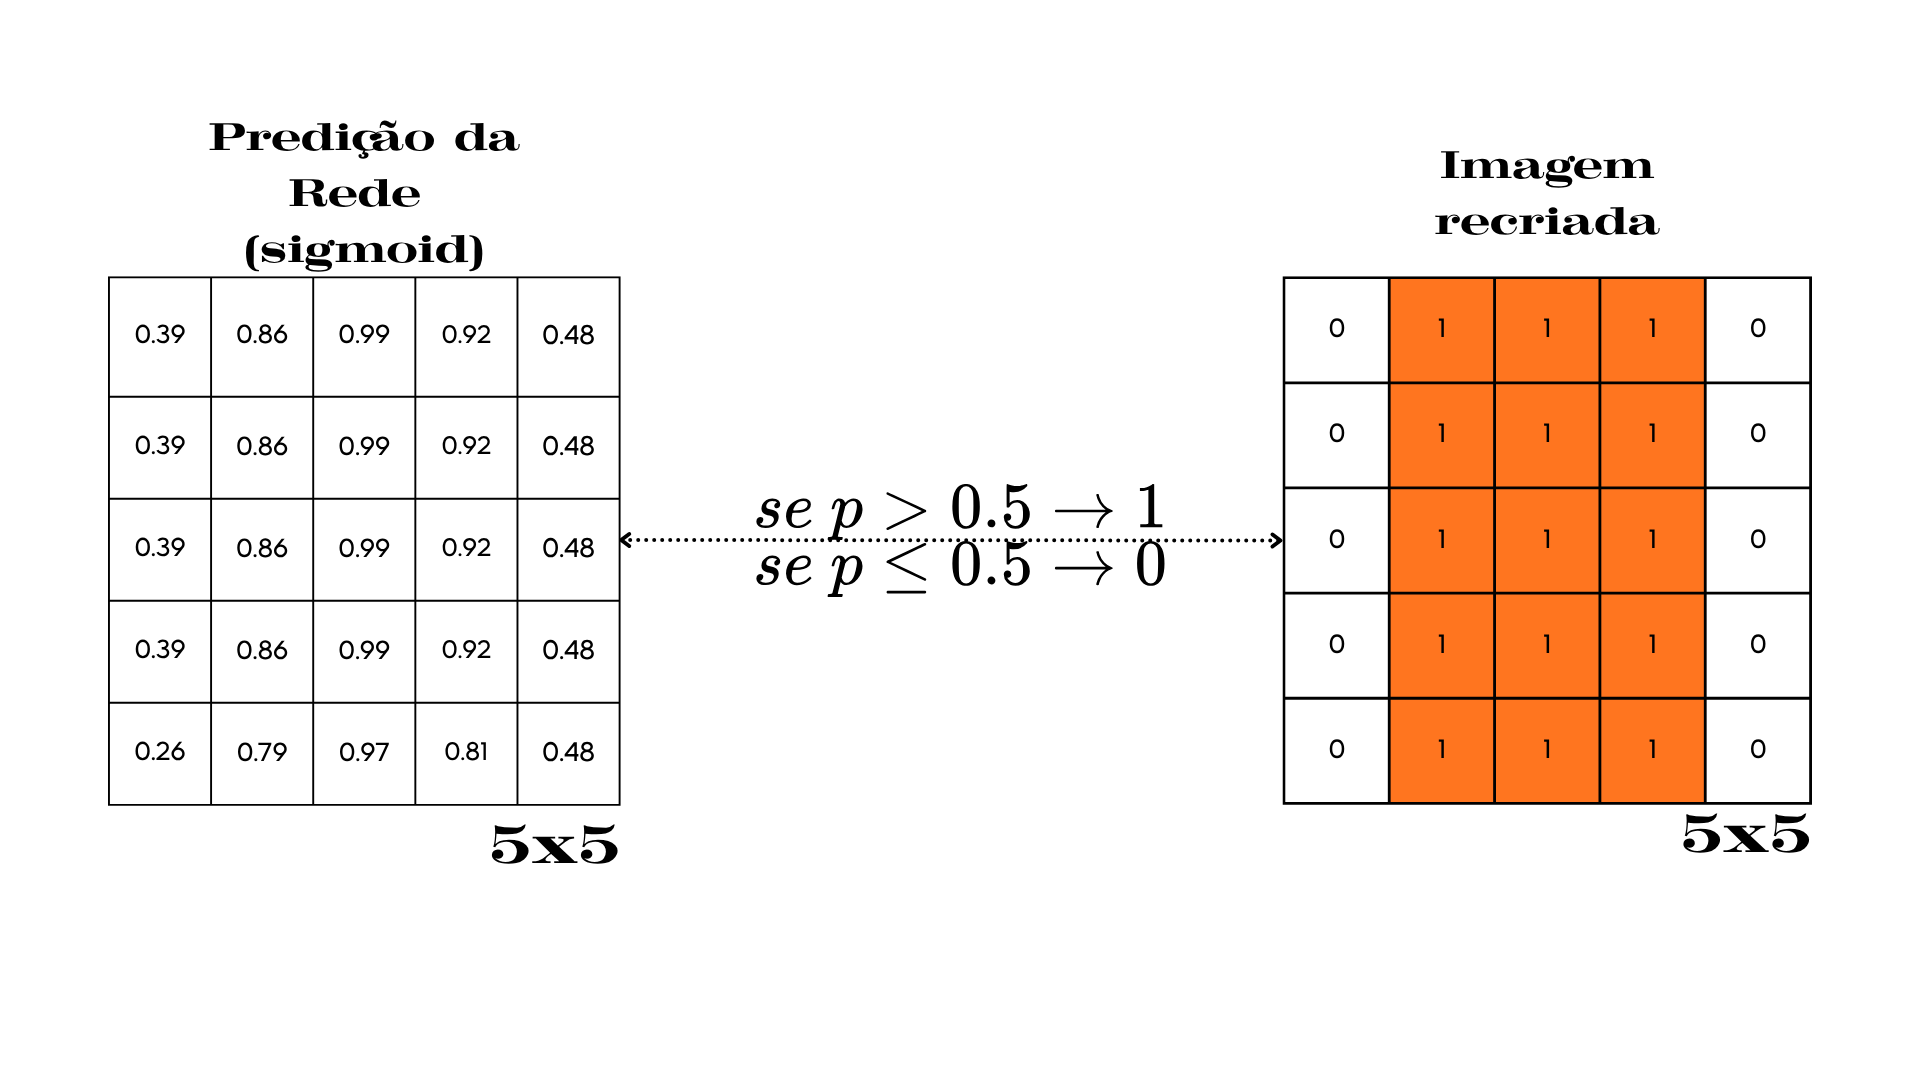
\includegraphics[width=0.8\linewidth]{figures/unetimgs/ex_fig11.png}
    \caption*{\footnotesize Fonte: Elaboração do Autor.}
    \label{ex:unet_img11}
\end{figure}
\end{exemplo}

\subsection{U-Net}
A rede convolucional desenvolvida por Ronneberger et al. \cite{Ronneberger2015UNet} é bem similar ao Exemplo \ref{ex:unet}, entretanto, a arquitetura completa da U-Net é composta por múltiplas camadas de convolução e pooling no encoder, e múltiplas camadas de convolução transposta no decoder, no total são quatro camadas de convolução e pooling no encoder e quatro camadas de convolução transposta no decoder, como mostra a Figura \ref{unet}. O número de filtros em cada camada de convolução aumenta à medida que se avança no encoder, começando com 64 filtros na primeira camada e dobrando a quantidade a cada camada subsequente, chegando a 1024 filtros na última camada do encoder. No decoder, o número de filtros é reduzido pela metade a cada camada subsequente, começando com 512 filtros na primeira camada do decoder e terminando com 64 filtros na última camada antes da saída. As conexões de atalho (\textit{skip connections}) entre as camadas correspondentes do encoder e do decoder permitem que sejam feitas as concatenações das imagens. A Figura \ref{unet} apresenta a arquitetura completa da U-Net, cada bloco representa uma etapa de processamento, o número na parte superior do bloco indica o número de filtros utilizados na camada de convolução, enquanto o número na parte inferior do bloco indica as dimensões espaciais da imagem resultante daquela etapa. A seta azul escuro representa a operação de convolução com filtros de dimenção $3\times 3$ e função de ativação $ReLU$, a seta vermelha representa a operação de pooling com \textit{kernel} de tamanho $2\times 2$ e stride de $2$, a seta cinza representa a operação de \textit{Copy and Crop} para realizar a concatenação das imagens, e a seta verde representa a operação de convolução transposta com filtros de dimensão $2\times 2$. A última camada de convolução utiliza um \textit{kernel} de dimensão $1\times 1$ e função de ativação \textit{sigmoid logística} (dependendo da aplicação) para gerar a imagem de saída segmentada.
\begin{figure}[H]
    \centering
    \caption{Arquitetura completa da U-Net.}
    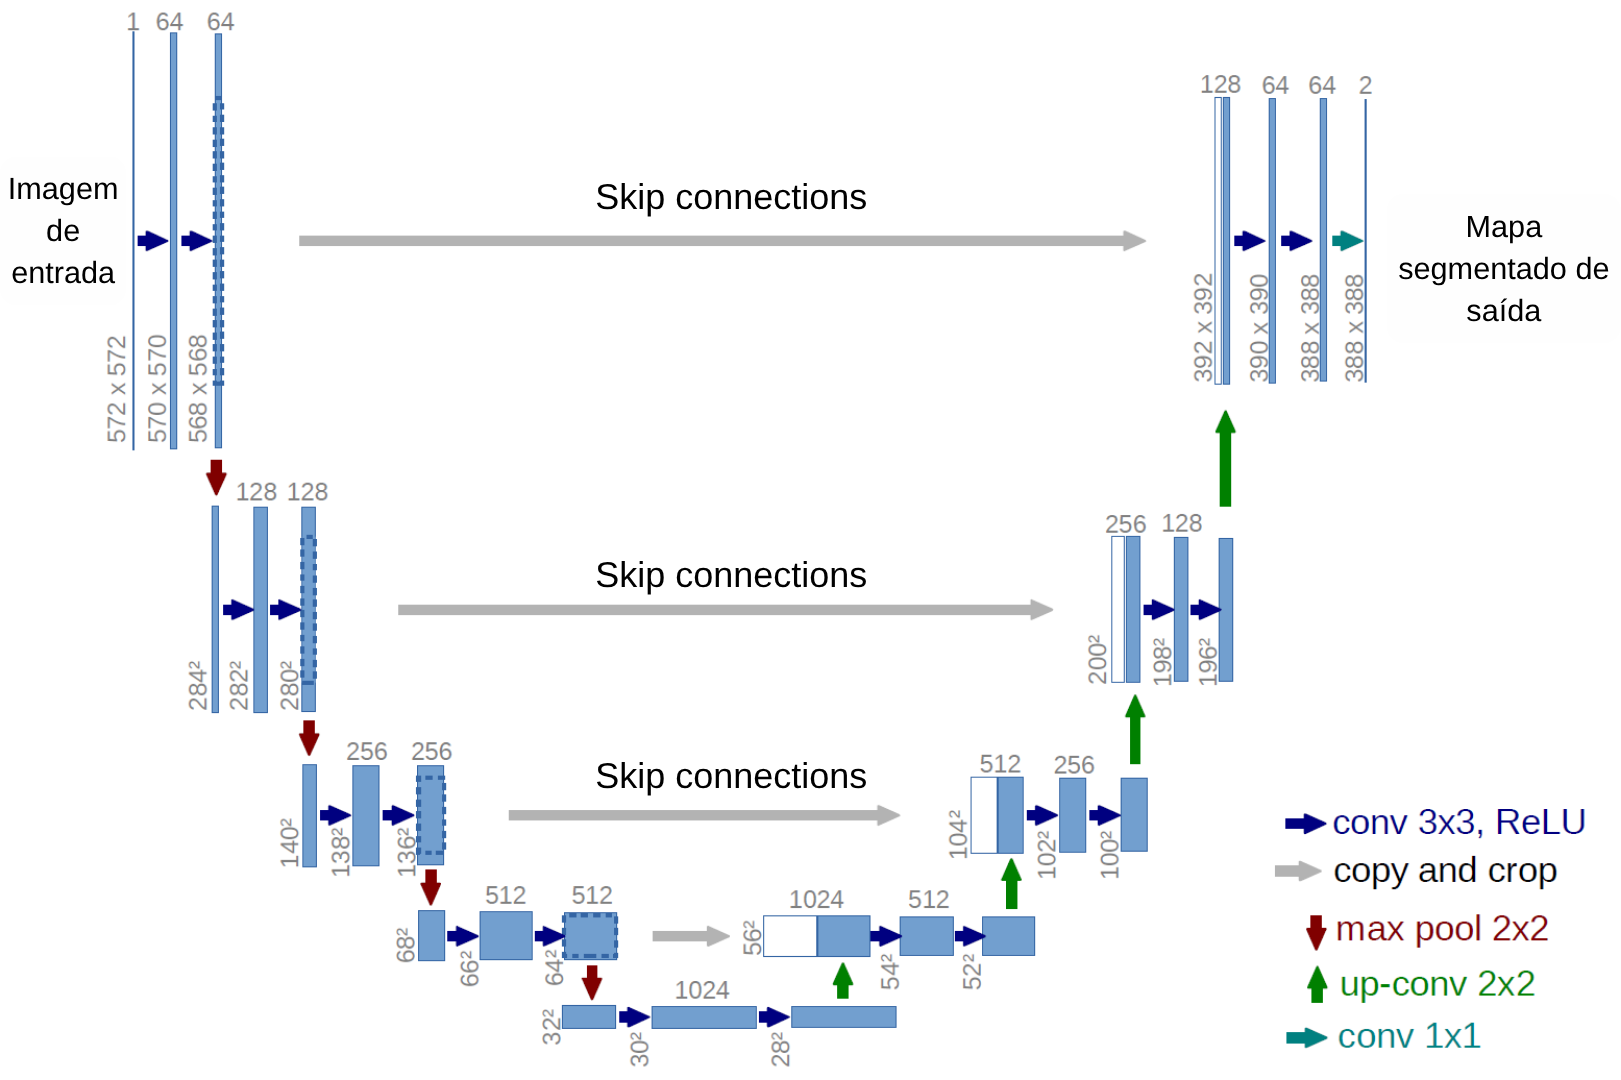
\includegraphics[width=0.8\linewidth]{figures/unetimgs/ex_unet.png}
    \caption*{\footnotesize Fonte: Adaptado de \cite{Ronneberger2015UNet}.}
    \label{unet}
\end{figure}
Como não é utilizado nenhum processo de \textit{padding} as dimensões da imagem são reduzidas em cada etapa de convolução. O corte feito para a concatenação (sinalizado por uma linha azul pontilhada) nas imagens do encoder (lado direito da Figura \ref{unet})  é feito no centro da imagem, ou seja, a parte central da imagem do encoder é mantida para a concatenação, enquanto as bordas são removidas. O total de parâmetros a serem otimizados é de aproximadamente $27.548,993$ dependendo da utilização do viés ou não. Para as duas primeiras camadas de convolução do encoder o número de parâmetros pode ser calculado da seguinte forma:
$$
\begin{array}{ccccc}
    & & &\\
    \text{1ª convolução} = & ((3 \times 3 \times 1) & + 1)& \times 64 & = 640 \\
    \text{2ª convolução} = & ((3 \times 3 \times 64) & + 1)& \times 64 & = 36.928.
\end{array}
$$

O filtro da segunda convolução tem 64 canais, um para cada mapa de características gerado pela primeira convolução, multiplica-se novamente por 64, pois cada filtro gera apenas um mapa de características.
\subsection{DICE}
